% Decision-Censored Learning -- ICML 2027 submission.
% The official icml2027.sty is not yet published; icml_substitute.sty matches
% the ICML geometry and macro API.  At submission: replace the \usepackage line
% below by \usepackage{icml2027} (with [accepted] for the camera-ready).
\documentclass{article}

\usepackage{icml_substitute}          % -> \usepackage{icml2027} at submission
\usepackage{amsmath,amssymb,amsthm,mathtools}
\usepackage{booktabs,multirow,array}
\usepackage{graphicx}
\usepackage{xcolor}
\usepackage[colorlinks=true,linkcolor=blue!50!black,citecolor=blue!50!black,
            urlcolor=blue!50!black]{hyperref}
\usepackage[capitalise,noabbrev]{cleveref}
\usepackage{natbib}
\usepackage{algorithm}
\usepackage{algpseudocode}
\usepackage{microtype}
\setlength{\emergencystretch}{2.5em}
% AUTO-GENERATED by scripts/make_numbers.py -- do not edit.
% Every number in the paper body is one of these macros (CLAUDE.md rule 2).
% Provenance for each macro: paper/numbers_provenance.json (rule 3).
\newcommand{\nCexAucHi}{0.4512}
\newcommand{\nCexAucLo}{0.4470}
\newcommand{\nCexAucMid}{0.4570}
\newcommand{\nCexAucPStar}{0.8252}
\newcommand{\nCexCornerWidth}{0.010}
\newcommand{\nCexMiss}{0.368}
\newcommand{\nCexPStarOne}{0.59}
\newcommand{\nCexPStarThree}{0.97}
\newcommand{\nCexPStarTwo}{0.98}
\newcommand{\nCexPloOne}{0.59}
\newcommand{\nCexPloThree}{0.48}
\newcommand{\nCexPloTwo}{0.85}
\newcommand{\nCexPupOne}{0.98}
\newcommand{\nCexPupThree}{0.97}
\newcommand{\nCexPupTwo}{0.98}
\newcommand{\nCexSharpHi}{0.8252}
\newcommand{\nCexSharpLo}{0.1341}
\newcommand{\nCexSharpWidth}{0.691}
\newcommand{\nCompasCornerCovAtORCI}{0\%}
\newcommand{\nCompasCornerCovAtOR}{0\%}
\newcommand{\nCompasCornerCovAtOneCI}{0\%}
\newcommand{\nCompasCornerCovAtOne}{0\%}
\newcommand{\nCompasCovAtORCI}{0\%}
\newcommand{\nCompasCovAtOR}{100\%}
\newcommand{\nCompasCovAtOneCI}{0\%}
\newcommand{\nCompasCovAtOne}{0\%}
\newcommand{\nCompasExpCornerCovAtORCI}{68\%}
\newcommand{\nCompasExpCornerCovAtOR}{40\%}
\newcommand{\nCompasExpCornerCovAtOneCI}{0\%}
\newcommand{\nCompasExpCornerCovAtOne}{0\%}
\newcommand{\nCompasExpCovAtORCI}{0\%}
\newcommand{\nCompasExpCovAtOR}{100\%}
\newcommand{\nCompasExpCovAtOneCI}{0\%}
\newcommand{\nCompasExpCovAtOne}{0\%}
\newcommand{\nCompasExpMAipwAurocCI}{0.0105}
\newcommand{\nCompasExpMAipwAuroc}{0.6950}
\newcommand{\nCompasExpMAipwObsAurocCI}{0.0166}
\newcommand{\nCompasExpMAipwObsAuroc}{0.6907}
\newcommand{\nCompasExpMAipwRegretCI}{0.0176}
\newcommand{\nCompasExpMAipwRegret}{0.1742}
\newcommand{\nCompasExpMAipwRiskCI}{0.0332}
\newcommand{\nCompasExpMAipwRisk}{0.7673}
\newcommand{\nCompasExpMAipwWcCI}{0.0150}
\newcommand{\nCompasExpMAipwWc}{0.8060}
\newcommand{\nCompasExpMDclOneFiveAurocCI}{\textbf{??}}
\newcommand{\nCompasExpMDclOneFiveAuroc}{\textbf{??}}
\newcommand{\nCompasExpMDclOneFiveObsAurocCI}{\textbf{??}}
\newcommand{\nCompasExpMDclOneFiveObsAuroc}{\textbf{??}}
\newcommand{\nCompasExpMDclOneFiveRegretCI}{\textbf{??}}
\newcommand{\nCompasExpMDclOneFiveRegret}{\textbf{??}}
\newcommand{\nCompasExpMDclOneFiveRiskCI}{\textbf{??}}
\newcommand{\nCompasExpMDclOneFiveRisk}{\textbf{??}}
\newcommand{\nCompasExpMDclOneFiveWcCI}{\textbf{??}}
\newcommand{\nCompasExpMDclOneFiveWc}{\textbf{??}}
\newcommand{\nCompasExpMDclRegOneFiveAurocCI}{\textbf{??}}
\newcommand{\nCompasExpMDclRegOneFiveAuroc}{\textbf{??}}
\newcommand{\nCompasExpMDclRegOneFiveObsAurocCI}{\textbf{??}}
\newcommand{\nCompasExpMDclRegOneFiveObsAuroc}{\textbf{??}}
\newcommand{\nCompasExpMDclRegOneFiveRegretCI}{\textbf{??}}
\newcommand{\nCompasExpMDclRegOneFiveRegret}{\textbf{??}}
\newcommand{\nCompasExpMDclRegOneFiveRiskCI}{\textbf{??}}
\newcommand{\nCompasExpMDclRegOneFiveRisk}{\textbf{??}}
\newcommand{\nCompasExpMDclRegOneFiveWcCI}{\textbf{??}}
\newcommand{\nCompasExpMDclRegOneFiveWc}{\textbf{??}}
\newcommand{\nCompasExpMDclRegThreeAurocCI}{0.0121}
\newcommand{\nCompasExpMDclRegThreeAuroc}{0.7142}
\newcommand{\nCompasExpMDclRegThreeObsAurocCI}{0.0184}
\newcommand{\nCompasExpMDclRegThreeObsAuroc}{0.7061}
\newcommand{\nCompasExpMDclRegThreeRegretCI}{0.0003}
\newcommand{\nCompasExpMDclRegThreeRegret}{0.0094}
\newcommand{\nCompasExpMDclRegThreeRiskCI}{0.0072}
\newcommand{\nCompasExpMDclRegThreeRisk}{0.6208}
\newcommand{\nCompasExpMDclRegThreeWcCI}{0.0052}
\newcommand{\nCompasExpMDclRegThreeWc}{0.6452}
\newcommand{\nCompasExpMDclRegTwoAurocCI}{0.0121}
\newcommand{\nCompasExpMDclRegTwoAuroc}{0.7139}
\newcommand{\nCompasExpMDclRegTwoObsAurocCI}{0.0185}
\newcommand{\nCompasExpMDclRegTwoObsAuroc}{0.7059}
\newcommand{\nCompasExpMDclRegTwoRegretCI}{0.0003}
\newcommand{\nCompasExpMDclRegTwoRegret}{0.0082}
\newcommand{\nCompasExpMDclRegTwoRiskCI}{0.0077}
\newcommand{\nCompasExpMDclRegTwoRisk}{0.6211}
\newcommand{\nCompasExpMDclRegTwoWcCI}{0.0052}
\newcommand{\nCompasExpMDclRegTwoWc}{0.6468}
\newcommand{\nCompasExpMDclThreeAurocCI}{0.0141}
\newcommand{\nCompasExpMDclThreeAuroc}{0.7088}
\newcommand{\nCompasExpMDclThreeObsAurocCI}{0.0187}
\newcommand{\nCompasExpMDclThreeObsAuroc}{0.7012}
\newcommand{\nCompasExpMDclThreeRegretCI}{0.0014}
\newcommand{\nCompasExpMDclThreeRegret}{0.0390}
\newcommand{\nCompasExpMDclThreeRiskCI}{0.0041}
\newcommand{\nCompasExpMDclThreeRisk}{0.6322}
\newcommand{\nCompasExpMDclThreeWcCI}{0.0051}
\newcommand{\nCompasExpMDclThreeWc}{0.6407}
\newcommand{\nCompasExpMDclTwoAurocCI}{0.0133}
\newcommand{\nCompasExpMDclTwoAuroc}{0.7139}
\newcommand{\nCompasExpMDclTwoObsAurocCI}{0.0191}
\newcommand{\nCompasExpMDclTwoObsAuroc}{0.7060}
\newcommand{\nCompasExpMDclTwoRegretCI}{0.0008}
\newcommand{\nCompasExpMDclTwoRegret}{0.0251}
\newcommand{\nCompasExpMDclTwoRiskCI}{0.0058}
\newcommand{\nCompasExpMDclTwoRisk}{0.6254}
\newcommand{\nCompasExpMDclTwoWcCI}{0.0051}
\newcommand{\nCompasExpMDclTwoWc}{0.6394}
\newcommand{\nCompasExpMErmAurocCI}{0.0106}
\newcommand{\nCompasExpMErmAuroc}{0.7014}
\newcommand{\nCompasExpMErmObsAurocCI}{0.0182}
\newcommand{\nCompasExpMErmObsAuroc}{0.6940}
\newcommand{\nCompasExpMErmRegretCI}{0.0084}
\newcommand{\nCompasExpMErmRegret}{0.0826}
\newcommand{\nCompasExpMErmRiskCI}{0.0176}
\newcommand{\nCompasExpMErmRisk}{0.6692}
\newcommand{\nCompasExpMErmWcCI}{0.0067}
\newcommand{\nCompasExpMErmWc}{0.7158}
\newcommand{\nCompasExpMHeckmanAurocCI}{0.0170}
\newcommand{\nCompasExpMHeckmanAurocMax}{0.748}
\newcommand{\nCompasExpMHeckmanAurocMin}{0.713}
\newcommand{\nCompasExpMHeckmanAuroc}{0.7249}
\newcommand{\nCompasExpMHeckmanObsAurocCI}{0.0275}
\newcommand{\nCompasExpMHeckmanObsAurocMax}{0.750}
\newcommand{\nCompasExpMHeckmanObsAurocMin}{0.693}
\newcommand{\nCompasExpMHeckmanObsAuroc}{0.7144}
\newcommand{\nCompasExpMHeckmanRegretCI}{0.0063}
\newcommand{\nCompasExpMHeckmanRegretMax}{0.130}
\newcommand{\nCompasExpMHeckmanRegretMin}{0.116}
\newcommand{\nCompasExpMHeckmanRegret}{0.1224}
\newcommand{\nCompasExpMHeckmanRiskCI}{0.0209}
\newcommand{\nCompasExpMHeckmanRiskMax}{0.647}
\newcommand{\nCompasExpMHeckmanRiskMin}{0.600}
\newcommand{\nCompasExpMHeckmanRisk}{0.6243}
\newcommand{\nCompasExpMHeckmanWcCI}{0.0060}
\newcommand{\nCompasExpMHeckmanWcMax}{0.738}
\newcommand{\nCompasExpMHeckmanWcMin}{0.727}
\newcommand{\nCompasExpMHeckmanWc}{0.7339}
\newcommand{\nCompasExpMImpAurocCI}{0.0111}
\newcommand{\nCompasExpMImpAuroc}{0.7052}
\newcommand{\nCompasExpMImpObsAurocCI}{0.0165}
\newcommand{\nCompasExpMImpObsAuroc}{0.6986}
\newcommand{\nCompasExpMImpRegretCI}{0.0042}
\newcommand{\nCompasExpMImpRegret}{0.0599}
\newcommand{\nCompasExpMImpRiskCI}{0.0124}
\newcommand{\nCompasExpMImpRisk}{0.6632}
\newcommand{\nCompasExpMImpWcCI}{0.0063}
\newcommand{\nCompasExpMImpWc}{0.6938}
\newcommand{\nCompasExpMIpwAurocCI}{0.0086}
\newcommand{\nCompasExpMIpwAuroc}{0.7001}
\newcommand{\nCompasExpMIpwObsAurocCI}{0.0156}
\newcommand{\nCompasExpMIpwObsAuroc}{0.6923}
\newcommand{\nCompasExpMIpwRegretCI}{0.0112}
\newcommand{\nCompasExpMIpwRegret}{0.0871}
\newcommand{\nCompasExpMIpwRiskCI}{0.0172}
\newcommand{\nCompasExpMIpwRisk}{0.6723}
\newcommand{\nCompasExpMIpwWcCI}{0.0098}
\newcommand{\nCompasExpMIpwWc}{0.7200}
\newcommand{\nCompasExpMManskiAurocCI}{0.0103}
\newcommand{\nCompasExpMManskiAuroc}{0.6075}
\newcommand{\nCompasExpMManskiObsAurocCI}{0.0148}
\newcommand{\nCompasExpMManskiObsAuroc}{0.6128}
\newcommand{\nCompasExpMManskiRegretCI}{0.0051}
\newcommand{\nCompasExpMManskiRegret}{0.1042}
\newcommand{\nCompasExpMManskiRiskCI}{0.0032}
\newcommand{\nCompasExpMManskiRisk}{0.6751}
\newcommand{\nCompasExpMManskiWcCI}{0.0032}
\newcommand{\nCompasExpMManskiWc}{0.6754}
\newcommand{\nCompasExpMOracleAurocCI}{0.0129}
\newcommand{\nCompasExpMOracleAuroc}{0.7121}
\newcommand{\nCompasExpMOracleObsAurocCI}{0.0208}
\newcommand{\nCompasExpMOracleObsAuroc}{0.7020}
\newcommand{\nCompasExpMOracleRegretCI}{0.0064}
\newcommand{\nCompasExpMOracleRegret}{0.0922}
\newcommand{\nCompasExpMOracleRiskCI}{0.0195}
\newcommand{\nCompasExpMOracleRisk}{0.6401}
\newcommand{\nCompasExpMOracleWcCI}{0.0054}
\newcommand{\nCompasExpMOracleWc}{0.7193}
\newcommand{\nCompasExpN}{4{,}957}
\newcommand{\nCompasExpOR}{2.135}
\newcommand{\nCompasExpObsMinusTrueCI}{+0.0079}
\newcommand{\nCompasExpObsMinusTrue}{-0.0053}
\newcommand{\nCompasExpRegretRatioErm}{10.1}
\newcommand{\nCompasExpRegretRatioHeckman}{14.9}
\newcommand{\nCompasExpWidthAtORCI}{0.002}
\newcommand{\nCompasExpWidthAtOR}{0.108}
\newcommand{\nCompasExpWidthAtOneCI}{0.000}
\newcommand{\nCompasExpWidthAtOne}{0.000}
\newcommand{\nCompasMAipwAurocCI}{0.0154}
\newcommand{\nCompasMAipwAuroc}{0.6950}
\newcommand{\nCompasMAipwObsAurocCI}{0.0188}
\newcommand{\nCompasMAipwObsAuroc}{0.6895}
\newcommand{\nCompasMAipwRegretCI}{0.0188}
\newcommand{\nCompasMAipwRegret}{0.1305}
\newcommand{\nCompasMAipwRiskCI}{0.0485}
\newcommand{\nCompasMAipwRisk}{0.7044}
\newcommand{\nCompasMAipwWcCI}{0.0125}
\newcommand{\nCompasMAipwWc}{0.7752}
\newcommand{\nCompasMDclOneFiveAurocCI}{\textbf{??}}
\newcommand{\nCompasMDclOneFiveAuroc}{\textbf{??}}
\newcommand{\nCompasMDclOneFiveObsAurocCI}{\textbf{??}}
\newcommand{\nCompasMDclOneFiveObsAuroc}{\textbf{??}}
\newcommand{\nCompasMDclOneFiveRegretCI}{\textbf{??}}
\newcommand{\nCompasMDclOneFiveRegret}{\textbf{??}}
\newcommand{\nCompasMDclOneFiveRiskCI}{\textbf{??}}
\newcommand{\nCompasMDclOneFiveRisk}{\textbf{??}}
\newcommand{\nCompasMDclOneFiveWcCI}{\textbf{??}}
\newcommand{\nCompasMDclOneFiveWc}{\textbf{??}}
\newcommand{\nCompasMDclRegOneFiveAurocCI}{\textbf{??}}
\newcommand{\nCompasMDclRegOneFiveAuroc}{\textbf{??}}
\newcommand{\nCompasMDclRegOneFiveObsAurocCI}{\textbf{??}}
\newcommand{\nCompasMDclRegOneFiveObsAuroc}{\textbf{??}}
\newcommand{\nCompasMDclRegOneFiveRegretCI}{\textbf{??}}
\newcommand{\nCompasMDclRegOneFiveRegret}{\textbf{??}}
\newcommand{\nCompasMDclRegOneFiveRiskCI}{\textbf{??}}
\newcommand{\nCompasMDclRegOneFiveRisk}{\textbf{??}}
\newcommand{\nCompasMDclRegOneFiveWcCI}{\textbf{??}}
\newcommand{\nCompasMDclRegOneFiveWc}{\textbf{??}}
\newcommand{\nCompasMDclRegThreeAurocCI}{0.0167}
\newcommand{\nCompasMDclRegThreeAuroc}{0.7109}
\newcommand{\nCompasMDclRegThreeObsAurocCI}{0.0209}
\newcommand{\nCompasMDclRegThreeObsAuroc}{0.7017}
\newcommand{\nCompasMDclRegThreeRegretCI}{0.0003}
\newcommand{\nCompasMDclRegThreeRegret}{0.0079}
\newcommand{\nCompasMDclRegThreeRiskCI}{0.0094}
\newcommand{\nCompasMDclRegThreeRisk}{0.6257}
\newcommand{\nCompasMDclRegThreeWcCI}{0.0070}
\newcommand{\nCompasMDclRegThreeWc}{0.6547}
\newcommand{\nCompasMDclRegTwoAurocCI}{0.0168}
\newcommand{\nCompasMDclRegTwoAuroc}{0.7106}
\newcommand{\nCompasMDclRegTwoObsAurocCI}{0.0212}
\newcommand{\nCompasMDclRegTwoObsAuroc}{0.7012}
\newcommand{\nCompasMDclRegTwoRegretCI}{0.0002}
\newcommand{\nCompasMDclRegTwoRegret}{0.0064}
\newcommand{\nCompasMDclRegTwoRiskCI}{0.0103}
\newcommand{\nCompasMDclRegTwoRisk}{0.6256}
\newcommand{\nCompasMDclRegTwoWcCI}{0.0069}
\newcommand{\nCompasMDclRegTwoWc}{0.6560}
\newcommand{\nCompasMDclThreeAurocCI}{0.0084}
\newcommand{\nCompasMDclThreeAuroc}{0.7043}
\newcommand{\nCompasMDclThreeObsAurocCI}{0.0160}
\newcommand{\nCompasMDclThreeObsAuroc}{0.6977}
\newcommand{\nCompasMDclThreeRegretCI}{0.0023}
\newcommand{\nCompasMDclThreeRegret}{0.0376}
\newcommand{\nCompasMDclThreeRiskCI}{0.0013}
\newcommand{\nCompasMDclThreeRisk}{0.6387}
\newcommand{\nCompasMDclThreeWcCI}{0.0067}
\newcommand{\nCompasMDclThreeWc}{0.6532}
\newcommand{\nCompasMDclTwoAurocCI}{0.0143}
\newcommand{\nCompasMDclTwoAuroc}{0.7096}
\newcommand{\nCompasMDclTwoObsAurocCI}{0.0194}
\newcommand{\nCompasMDclTwoObsAuroc}{0.7009}
\newcommand{\nCompasMDclTwoRegretCI}{0.0009}
\newcommand{\nCompasMDclTwoRegret}{0.0238}
\newcommand{\nCompasMDclTwoRiskCI}{0.0036}
\newcommand{\nCompasMDclTwoRisk}{0.6309}
\newcommand{\nCompasMDclTwoWcCI}{0.0070}
\newcommand{\nCompasMDclTwoWc}{0.6506}
\newcommand{\nCompasMErmAurocCI}{0.0157}
\newcommand{\nCompasMErmAuroc}{0.6991}
\newcommand{\nCompasMErmObsAurocCI}{0.0220}
\newcommand{\nCompasMErmObsAuroc}{0.6898}
\newcommand{\nCompasMErmRegretCI}{0.0030}
\newcommand{\nCompasMErmRegret}{0.0698}
\newcommand{\nCompasMErmRiskCI}{0.0249}
\newcommand{\nCompasMErmRisk}{0.6548}
\newcommand{\nCompasMErmWcCI}{0.0096}
\newcommand{\nCompasMErmWc}{0.7154}
\newcommand{\nCompasMHeckmanAurocCI}{0.0097}
\newcommand{\nCompasMHeckmanAurocMax}{0.728}
\newcommand{\nCompasMHeckmanAurocMin}{0.711}
\newcommand{\nCompasMHeckmanAuroc}{0.7212}
\newcommand{\nCompasMHeckmanObsAurocCI}{0.0164}
\newcommand{\nCompasMHeckmanObsAurocMax}{0.728}
\newcommand{\nCompasMHeckmanObsAurocMin}{0.696}
\newcommand{\nCompasMHeckmanObsAuroc}{0.7133}
\newcommand{\nCompasMHeckmanRegretCI}{0.0134}
\newcommand{\nCompasMHeckmanRegretMax}{0.123}
\newcommand{\nCompasMHeckmanRegretMin}{0.095}
\newcommand{\nCompasMHeckmanRegret}{0.1041}
\newcommand{\nCompasMHeckmanRiskCI}{0.0081}
\newcommand{\nCompasMHeckmanRiskMax}{0.633}
\newcommand{\nCompasMHeckmanRiskMin}{0.616}
\newcommand{\nCompasMHeckmanRisk}{0.6245}
\newcommand{\nCompasMHeckmanWcCI}{0.0205}
\newcommand{\nCompasMHeckmanWcMax}{0.756}
\newcommand{\nCompasMHeckmanWcMin}{0.713}
\newcommand{\nCompasMHeckmanWc}{0.7293}
\newcommand{\nCompasMImpAurocCI}{0.0135}
\newcommand{\nCompasMImpAuroc}{0.7036}
\newcommand{\nCompasMImpObsAurocCI}{0.0183}
\newcommand{\nCompasMImpObsAuroc}{0.6962}
\newcommand{\nCompasMImpRegretCI}{0.0029}
\newcommand{\nCompasMImpRegret}{0.0446}
\newcommand{\nCompasMImpRiskCI}{0.0152}
\newcommand{\nCompasMImpRisk}{0.6434}
\newcommand{\nCompasMImpWcCI}{0.0099}
\newcommand{\nCompasMImpWc}{0.6908}
\newcommand{\nCompasMIpwAurocCI}{0.0158}
\newcommand{\nCompasMIpwAuroc}{0.6977}
\newcommand{\nCompasMIpwObsAurocCI}{0.0204}
\newcommand{\nCompasMIpwObsAuroc}{0.6891}
\newcommand{\nCompasMIpwRegretCI}{0.0037}
\newcommand{\nCompasMIpwRegret}{0.0727}
\newcommand{\nCompasMIpwRiskCI}{0.0254}
\newcommand{\nCompasMIpwRisk}{0.6571}
\newcommand{\nCompasMIpwWcCI}{0.0098}
\newcommand{\nCompasMIpwWc}{0.7183}
\newcommand{\nCompasMManskiAurocCI}{0.0096}
\newcommand{\nCompasMManskiAuroc}{0.5869}
\newcommand{\nCompasMManskiObsAurocCI}{0.0101}
\newcommand{\nCompasMManskiObsAuroc}{0.5976}
\newcommand{\nCompasMManskiRegretCI}{0.0119}
\newcommand{\nCompasMManskiRegret}{0.0911}
\newcommand{\nCompasMManskiRiskCI}{0.0005}
\newcommand{\nCompasMManskiRisk}{0.6804}
\newcommand{\nCompasMManskiWcCI}{0.0010}
\newcommand{\nCompasMManskiWc}{0.6833}
\newcommand{\nCompasMOracleAurocCI}{0.0117}
\newcommand{\nCompasMOracleAuroc}{0.7115}
\newcommand{\nCompasMOracleObsAurocCI}{0.0191}
\newcommand{\nCompasMOracleObsAuroc}{0.7010}
\newcommand{\nCompasMOracleRegretCI}{0.0074}
\newcommand{\nCompasMOracleRegret}{0.0798}
\newcommand{\nCompasMOracleRiskCI}{0.0150}
\newcommand{\nCompasMOracleRisk}{0.6309}
\newcommand{\nCompasMOracleWcCI}{0.0153}
\newcommand{\nCompasMOracleWc}{0.7197}
\newcommand{\nCompasN}{6{,}054}
\newcommand{\nCompasOR}{1.885}
\newcommand{\nCompasObsMinusTrueCI}{+0.0093}
\newcommand{\nCompasObsMinusTrue}{-0.0076}
\newcommand{\nCompasRegretRatioErm}{10.9}
\newcommand{\nCompasRegretRatioHeckman}{16.3}
\newcommand{\nCompasTarCustodyDetainedMedian}{10.1}
\newcommand{\nCompasTarCustodyDetainedQNinety}{68}
\newcommand{\nCompasTarCustodyReleasedMedian}{0.9}
\newcommand{\nCompasTarKeptDetainedPct}{79\%}
\newcommand{\nCompasTarKeptPct}{82\%}
\newcommand{\nCompasTarNCohort}{6{,}054}
\newcommand{\nCompasTarNPropublica}{6{,}172}
\newcommand{\nCompasTarNRaw}{7{,}214}
\newcommand{\nCompasTarORExposure}{2.14}
\newcommand{\nCompasTarORRecorded}{1.88}
\newcommand{\nCompasTarPOneExposure}{38\%}
\newcommand{\nCompasTarPOneRecorded}{39\%}
\newcommand{\nCompasTarPZeroExposure}{57\%}
\newcommand{\nCompasTarPZeroRecorded}{55\%}
\newcommand{\nCompasTarSelectionPct}{63\%}
\newcommand{\nCompasWidthAtORCI}{0.002}
\newcommand{\nCompasWidthAtOR}{0.099}
\newcommand{\nCompasWidthAtOneCI}{0.000}
\newcommand{\nCompasWidthAtOne}{0.000}
\newcommand{\nExpEightAlphaPct}{10}
\newcommand{\nExpEightCompasAucCovBinsTwentyCI}{\textbf{??}}
\newcommand{\nExpEightCompasAucCovBinsTwenty}{\textbf{??}}
\newcommand{\nExpEightCompasAucCovEmpBinsTwentyCI}{0.0\%}
\newcommand{\nExpEightCompasAucCovEmpBinsTwenty}{100.0\%}
\newcommand{\nExpEightCompasAucCovEmpPluginCI}{55.5\%}
\newcommand{\nExpEightCompasAucCovEmpPlugin}{80.0\%}
\newcommand{\nExpEightCompasAucCovPluginCI}{\textbf{??}}
\newcommand{\nExpEightCompasAucCovPlugin}{\textbf{??}}
\newcommand{\nExpEightCompasAucWidthBinsTwentyCI}{0.016}
\newcommand{\nExpEightCompasAucWidthBinsTwenty}{0.388}
\newcommand{\nExpEightCompasAucWidthPluginCI}{0.003}
\newcommand{\nExpEightCompasAucWidthPlugin}{0.099}
\newcommand{\nExpEightCompasBinCovBinsTwentyCI}{0.0\%}
\newcommand{\nExpEightCompasBinCovBinsTwenty}{100.0\%}
\newcommand{\nExpEightCompasBinCovPluginCI}{5.6\%}
\newcommand{\nExpEightCompasBinCovPlugin}{98.0\%}
\newcommand{\nExpEightCompasCovBinsTenCI}{\textbf{??}}
\newcommand{\nExpEightCompasCovBinsTenSmoothCI}{\textbf{??}}
\newcommand{\nExpEightCompasCovBinsTenSmooth}{\textbf{??}}
\newcommand{\nExpEightCompasCovBinsTen}{\textbf{??}}
\newcommand{\nExpEightCompasCovBinsTwentyCI}{\textbf{??}}
\newcommand{\nExpEightCompasCovBinsTwentySmoothCI}{\textbf{??}}
\newcommand{\nExpEightCompasCovBinsTwentySmooth}{\textbf{??}}
\newcommand{\nExpEightCompasCovBinsTwenty}{\textbf{??}}
\newcommand{\nExpEightCompasCovOracleECI}{\textbf{??}}
\newcommand{\nExpEightCompasCovOracleE}{\textbf{??}}
\newcommand{\nExpEightCompasCovOraclePCI}{\textbf{??}}
\newcommand{\nExpEightCompasCovOracleP}{\textbf{??}}
\newcommand{\nExpEightCompasCovPluginCI}{\textbf{??}}
\newcommand{\nExpEightCompasCovPlugin}{\textbf{??}}
\newcommand{\nExpEightCompasDrCovPrevCI}{\textbf{??}}
\newcommand{\nExpEightCompasDrCovPrev}{\textbf{??}}
\newcommand{\nExpEightCompasDrCovRealisedCI}{0.0\%}
\newcommand{\nExpEightCompasDrCovRealised}{100.0\%}
\newcommand{\nExpEightCompasDrErrHiCI}{\textbf{??}}
\newcommand{\nExpEightCompasDrErrHi}{\textbf{??}}
\newcommand{\nExpEightCompasDrErrLoCI}{\textbf{??}}
\newcommand{\nExpEightCompasDrErrLo}{\textbf{??}}
\newcommand{\nExpEightCompasMaeECI}{\textbf{??}}
\newcommand{\nExpEightCompasMaeE}{\textbf{??}}
\newcommand{\nExpEightCompasMaePCI}{\textbf{??}}
\newcommand{\nExpEightCompasMaeP}{\textbf{??}}
\newcommand{\nExpEightCompasPlugCovPrevCI}{\textbf{??}}
\newcommand{\nExpEightCompasPlugCovPrev}{\textbf{??}}
\newcommand{\nExpEightCompasPlugErrHiCI}{\textbf{??}}
\newcommand{\nExpEightCompasPlugErrHi}{\textbf{??}}
\newcommand{\nExpEightCompasPlugErrLoCI}{\textbf{??}}
\newcommand{\nExpEightCompasPlugErrLo}{\textbf{??}}
\newcommand{\nExpEightCompasWidthBinsTwentyCI}{0.013}
\newcommand{\nExpEightCompasWidthBinsTwentySmoothCI}{0.023}
\newcommand{\nExpEightCompasWidthBinsTwentySmooth}{0.466}
\newcommand{\nExpEightCompasWidthBinsTwenty}{0.390}
\newcommand{\nExpEightCompasWidthPluginCI}{0.002}
\newcommand{\nExpEightCompasWidthPlugin}{0.102}
\newcommand{\nExpEightLendingAucCovBinsTwentyCI}{0.0\%}
\newcommand{\nExpEightLendingAucCovBinsTwenty}{100.0\%}
\newcommand{\nExpEightLendingAucCovEmpBinsTwentyCI}{0.0\%}
\newcommand{\nExpEightLendingAucCovEmpBinsTwenty}{100.0\%}
\newcommand{\nExpEightLendingAucCovEmpPluginCI}{55.5\%}
\newcommand{\nExpEightLendingAucCovEmpPlugin}{80.0\%}
\newcommand{\nExpEightLendingAucCovPluginCI}{55.5\%}
\newcommand{\nExpEightLendingAucCovPlugin}{80.0\%}
\newcommand{\nExpEightLendingAucWidthBinsTwentyCI}{0.016}
\newcommand{\nExpEightLendingAucWidthBinsTwenty}{0.636}
\newcommand{\nExpEightLendingAucWidthPluginCI}{0.002}
\newcommand{\nExpEightLendingAucWidthPlugin}{0.137}
\newcommand{\nExpEightLendingBinCovBinsTwentyCI}{\textbf{??}}
\newcommand{\nExpEightLendingBinCovBinsTwenty}{\textbf{??}}
\newcommand{\nExpEightLendingBinCovPluginCI}{\textbf{??}}
\newcommand{\nExpEightLendingBinCovPlugin}{\textbf{??}}
\newcommand{\nExpEightLendingCovBinsTenCI}{3.1\%}
\newcommand{\nExpEightLendingCovBinsTenSmoothCI}{1.8\%}
\newcommand{\nExpEightLendingCovBinsTenSmooth}{97.1\%}
\newcommand{\nExpEightLendingCovBinsTen}{93.0\%}
\newcommand{\nExpEightLendingCovBinsTwentyCI}{0.9\%}
\newcommand{\nExpEightLendingCovBinsTwentySmoothCI}{0.8\%}
\newcommand{\nExpEightLendingCovBinsTwentySmooth}{98.2\%}
\newcommand{\nExpEightLendingCovBinsTwenty}{97.2\%}
\newcommand{\nExpEightLendingCovOracleECI}{5.3\%}
\newcommand{\nExpEightLendingCovOracleE}{43.8\%}
\newcommand{\nExpEightLendingCovOraclePCI}{0.0\%}
\newcommand{\nExpEightLendingCovOracleP}{100.0\%}
\newcommand{\nExpEightLendingCovPluginCI}{5.6\%}
\newcommand{\nExpEightLendingCovPlugin}{44.1\%}
\newcommand{\nExpEightLendingDrCovPrevCI}{0.0\%}
\newcommand{\nExpEightLendingDrCovPrev}{100.0\%}
\newcommand{\nExpEightLendingDrCovRealisedCI}{0.0\%}
\newcommand{\nExpEightLendingDrCovRealised}{100.0\%}
\newcommand{\nExpEightLendingDrErrHiCI}{0.005}
\newcommand{\nExpEightLendingDrErrHi}{0.010}
\newcommand{\nExpEightLendingDrErrLoCI}{0.003}
\newcommand{\nExpEightLendingDrErrLo}{0.005}
\newcommand{\nExpEightLendingMaeECI}{0.002}
\newcommand{\nExpEightLendingMaeE}{0.080}
\newcommand{\nExpEightLendingMaePCI}{0.003}
\newcommand{\nExpEightLendingMaeP}{0.018}
\newcommand{\nExpEightLendingPlugCovPrevCI}{0.0\%}
\newcommand{\nExpEightLendingPlugCovPrev}{0.0\%}
\newcommand{\nExpEightLendingPlugErrHiCI}{0.004}
\newcommand{\nExpEightLendingPlugErrHi}{0.008}
\newcommand{\nExpEightLendingPlugErrLoCI}{0.001}
\newcommand{\nExpEightLendingPlugErrLo}{0.005}
\newcommand{\nExpEightLendingWidthBinsTwentyCI}{0.008}
\newcommand{\nExpEightLendingWidthBinsTwentySmoothCI}{0.014}
\newcommand{\nExpEightLendingWidthBinsTwentySmooth}{0.201}
\newcommand{\nExpEightLendingWidthBinsTwenty}{0.153}
\newcommand{\nExpEightLendingWidthPluginCI}{0.002}
\newcommand{\nExpEightLendingWidthPlugin}{0.026}
\newcommand{\nExpEightSeeds}{5}
\newcommand{\nExpEightSlBenchAucCovBinsTwentyCI}{0.0\%}
\newcommand{\nExpEightSlBenchAucCovBinsTwenty}{100.0\%}
\newcommand{\nExpEightSlBenchAucCovEmpBinsTwentyCI}{0.0\%}
\newcommand{\nExpEightSlBenchAucCovEmpBinsTwenty}{100.0\%}
\newcommand{\nExpEightSlBenchAucCovEmpPluginCI}{0.0\%}
\newcommand{\nExpEightSlBenchAucCovEmpPlugin}{100.0\%}
\newcommand{\nExpEightSlBenchAucCovPluginCI}{0.0\%}
\newcommand{\nExpEightSlBenchAucCovPlugin}{100.0\%}
\newcommand{\nExpEightSlBenchAucWidthBinsTwentyCI}{0.025}
\newcommand{\nExpEightSlBenchAucWidthBinsTwenty}{0.444}
\newcommand{\nExpEightSlBenchAucWidthPluginCI}{0.013}
\newcommand{\nExpEightSlBenchAucWidthPlugin}{0.243}
\newcommand{\nExpEightSlBenchBinCovBinsTwentyCI}{\textbf{??}}
\newcommand{\nExpEightSlBenchBinCovBinsTwenty}{\textbf{??}}
\newcommand{\nExpEightSlBenchBinCovPluginCI}{\textbf{??}}
\newcommand{\nExpEightSlBenchBinCovPlugin}{\textbf{??}}
\newcommand{\nExpEightSlBenchCovBinsTenCI}{5.3\%}
\newcommand{\nExpEightSlBenchCovBinsTenSmoothCI}{2.4\%}
\newcommand{\nExpEightSlBenchCovBinsTenSmooth}{94.7\%}
\newcommand{\nExpEightSlBenchCovBinsTen}{84.3\%}
\newcommand{\nExpEightSlBenchCovBinsTwentyCI}{3.8\%}
\newcommand{\nExpEightSlBenchCovBinsTwentySmoothCI}{2.5\%}
\newcommand{\nExpEightSlBenchCovBinsTwentySmooth}{94.5\%}
\newcommand{\nExpEightSlBenchCovBinsTwenty}{90.5\%}
\newcommand{\nExpEightSlBenchCovOracleECI}{8.9\%}
\newcommand{\nExpEightSlBenchCovOracleE}{54.8\%}
\newcommand{\nExpEightSlBenchCovOraclePCI}{5.7\%}
\newcommand{\nExpEightSlBenchCovOracleP}{89.7\%}
\newcommand{\nExpEightSlBenchCovPluginCI}{7.6\%}
\newcommand{\nExpEightSlBenchCovPlugin}{55.4\%}
\newcommand{\nExpEightSlBenchDrCovPrevCI}{0.0\%}
\newcommand{\nExpEightSlBenchDrCovPrev}{100.0\%}
\newcommand{\nExpEightSlBenchDrCovRealisedCI}{0.0\%}
\newcommand{\nExpEightSlBenchDrCovRealised}{100.0\%}
\newcommand{\nExpEightSlBenchDrErrHiCI}{0.004}
\newcommand{\nExpEightSlBenchDrErrHi}{0.007}
\newcommand{\nExpEightSlBenchDrErrLoCI}{0.008}
\newcommand{\nExpEightSlBenchDrErrLo}{0.006}
\newcommand{\nExpEightSlBenchMaeECI}{0.003}
\newcommand{\nExpEightSlBenchMaeE}{0.065}
\newcommand{\nExpEightSlBenchMaePCI}{0.009}
\newcommand{\nExpEightSlBenchMaeP}{0.069}
\newcommand{\nExpEightSlBenchPlugCovPrevCI}{0.0\%}
\newcommand{\nExpEightSlBenchPlugCovPrev}{0.0\%}
\newcommand{\nExpEightSlBenchPlugErrHiCI}{0.009}
\newcommand{\nExpEightSlBenchPlugErrHi}{0.011}
\newcommand{\nExpEightSlBenchPlugErrLoCI}{0.012}
\newcommand{\nExpEightSlBenchPlugErrLo}{0.009}
\newcommand{\nExpEightSlBenchWidthBinsTwentyCI}{0.022}
\newcommand{\nExpEightSlBenchWidthBinsTwentySmoothCI}{0.020}
\newcommand{\nExpEightSlBenchWidthBinsTwentySmooth}{0.481}
\newcommand{\nExpEightSlBenchWidthBinsTwenty}{0.405}
\newcommand{\nExpEightSlBenchWidthPluginCI}{0.015}
\newcommand{\nExpEightSlBenchWidthPlugin}{0.219}
\newcommand{\nExpFiveCoefGrowthPct}{25}
\newcommand{\nExpFiveDevRate}{-0.507}
\newcommand{\nExpFiveExcessRate}{-1.08}
\newcommand{\nExpFiveGammaRange}{16}
\newcommand{\nExpFiveOneFiveB}{5.37}
\newcommand{\nExpFiveOneFiveCoef}{2.243}
\newcommand{\nExpFiveOneFiveRate}{-0.519}
\newcommand{\nExpFiveRateMax}{-0.490}
\newcommand{\nExpFiveRateMin}{-0.534}
\newcommand{\nExpFiveRtwoLin}{0.60}
\newcommand{\nExpFiveRtwoLog}{0.89}
\newcommand{\nExpFiveSeedsDev}{8}
\newcommand{\nExpFiveSixB}{6.76}
\newcommand{\nExpFiveSixCoef}{2.687}
\newcommand{\nExpFiveSixRate}{-0.534}
\newcommand{\nExpFiveThreeB}{6.06}
\newcommand{\nExpFiveThreeCoef}{2.468}
\newcommand{\nExpFiveThreeRate}{-0.490}
\newcommand{\nExpFiveTwelveB}{7.45}
\newcommand{\nExpFiveTwelveCoef}{2.804}
\newcommand{\nExpFiveTwelveRate}{-0.491}
\newcommand{\nExpFiveTwentyFourB}{8.14}
\newcommand{\nExpFiveTwentyFourCoef}{2.775}
\newcommand{\nExpFiveTwentyFourRate}{-0.491}
\newcommand{\nExpFiveTwoB}{5.66}
\newcommand{\nExpFiveTwoCoef}{2.377}
\newcommand{\nExpFiveTwoRate}{-0.514}
\newcommand{\nExpFourFalseAlarm}{0\%}
\newcommand{\nExpFourFiveHetGminQ}{2.42}
\newcommand{\nExpFourFiveHetGmin}{4.42}
\newcommand{\nExpFourFiveHetGzCond}{11.19}
\newcommand{\nExpFourFiveHetRec}{0.34}
\newcommand{\nExpFourFiveHomGminQ}{2.27}
\newcommand{\nExpFourFiveHomGmin}{3.17}
\newcommand{\nExpFourFiveHomGzCond}{7.62}
\newcommand{\nExpFourFiveHomRec}{0.37}
\newcommand{\nExpFourGminAtThree}{1.91}
\newcommand{\nExpFourLendingBreakEvenFiftyFive}{1.72}
\newcommand{\nExpFourLendingBreakEvenFifty}{2.82}
\newcommand{\nExpFourLendingBreakEvenSixty}{1.05}
\newcommand{\nExpFourLendingDclBeatsUpto}{40.00}
\newcommand{\nExpFourMimicSimBreakEvenFiftyFive}{9.10}
\newcommand{\nExpFourMimicSimBreakEvenFifty}{14.91}
\newcommand{\nExpFourMimicSimBreakEvenSixty}{5.55}
\newcommand{\nExpFourMimicSimDclBeatsUpto}{40.00}
\newcommand{\nExpFourMisCovHigh}{100\%}
\newcommand{\nExpFourMisCovLow}{70\%}
\newcommand{\nExpFourMisRange}{12}
\newcommand{\nExpFourMisSeeds}{5}
\newcommand{\nExpFourMisWidthHigh}{0.40}
\newcommand{\nExpFourMisWidthLow}{0.04}
\newcommand{\nExpFourMisWidthMax}{0.41}
\newcommand{\nExpFourMisWidthMin}{0.00}
\newcommand{\nExpFourNCells}{30}
\newcommand{\nExpFourOneFiveHetGminQ}{1.40}
\newcommand{\nExpFourOneFiveHetGmin}{1.57}
\newcommand{\nExpFourOneFiveHetGzCond}{1.86}
\newcommand{\nExpFourOneFiveHetRec}{0.51}
\newcommand{\nExpFourOneFiveHomGminQ}{1.34}
\newcommand{\nExpFourOneFiveHomGmin}{1.42}
\newcommand{\nExpFourOneFiveHomGzCond}{1.58}
\newcommand{\nExpFourOneFiveHomRec}{0.61}
\newcommand{\nExpFourOneHetGminQ}{1.00}
\newcommand{\nExpFourOneHetGmin}{1.00}
\newcommand{\nExpFourOneHetGzCond}{1.00}
\newcommand{\nExpFourOneHetRec}{nan}
\newcommand{\nExpFourOneHomGminQ}{1.00}
\newcommand{\nExpFourOneHomGmin}{1.00}
\newcommand{\nExpFourOneHomGzCond}{1.00}
\newcommand{\nExpFourOneHomRec}{nan}
\newcommand{\nExpFourRecoverMax}{81\%}
\newcommand{\nExpFourRecoverMin}{21\%}
\newcommand{\nExpFourRefutesMar}{100\%}
\newcommand{\nExpFourSeedsMis}{5}
\newcommand{\nExpFourSlBenchBreakEvenFiftyFive}{1.62}
\newcommand{\nExpFourSlBenchBreakEvenFifty}{2.49}
\newcommand{\nExpFourSlBenchBreakEvenSixty}{1.05}
\newcommand{\nExpFourSlBenchDclBeatsUpto}{40.00}
\newcommand{\nExpFourThreeHetGminQ}{2.05}
\newcommand{\nExpFourThreeHetGmin}{3.16}
\newcommand{\nExpFourThreeHetGzCond}{5.45}
\newcommand{\nExpFourThreeHetRec}{0.39}
\newcommand{\nExpFourThreeHomGminQ}{1.91}
\newcommand{\nExpFourThreeHomGmin}{2.41}
\newcommand{\nExpFourThreeHomGzCond}{3.83}
\newcommand{\nExpFourThreeHomRec}{0.45}
\newcommand{\nExpFourTwoHetGminQ}{1.69}
\newcommand{\nExpFourTwoHetGmin}{2.18}
\newcommand{\nExpFourTwoHetGzCond}{2.92}
\newcommand{\nExpFourTwoHetRec}{0.45}
\newcommand{\nExpFourTwoHomGminQ}{1.59}
\newcommand{\nExpFourTwoHomGmin}{1.81}
\newcommand{\nExpFourTwoHomGzCond}{2.27}
\newcommand{\nExpFourTwoHomRec}{0.54}
\newcommand{\nExpFourValid}{yes}
\newcommand{\nExpNineEqualInstances}{4{,}160}
\newcommand{\nExpNineEqualViolations}{0}
\newcommand{\nExpNineFamilyPct}{94\%}
\newcommand{\nExpNineLoBeatenPct}{41\%}
\newcommand{\nExpNineMidBeatenPct}{30\%}
\newcommand{\nExpNineMidBeatenSevenPct}{83\%}
\newcommand{\nExpNineMidGapMax}{0.15}
\newcommand{\nExpNineMidGapMean}{0.006}
\newcommand{\nExpNineNMax}{7}
\newcommand{\nExpNineUnequalInstances}{4{,}160}
\newcommand{\nExpOneAttain}{1.2\times10^{-15}}
\newcommand{\nExpOneCovCorner}{10\%}
\newcommand{\nExpOneCovSeparate}{100\%}
\newcommand{\nExpOneCovSharpEmp}{100\%}
\newcommand{\nExpOneCovSharp}{100\%}
\newcommand{\nExpOneCovTooSmall}{71\%}
\newcommand{\nExpOneGap}{3.6\times10^{-6}}
\newcommand{\nExpOneNCells}{24}
\newcommand{\nExpOneNInstances}{120}
\newcommand{\nExpOneRuntimeFourHundredK}{2.5}
\newcommand{\nExpOneRuntimeHundredK}{0.61}
\newcommand{\nExpOneRuntimeTwentyK}{0.11}
\newcommand{\nExpOneSeeds}{5}
\newcommand{\nExpOneWidthCorner}{0.018}
\newcommand{\nExpOneWidthRatioCorner}{15.3}
\newcommand{\nExpOneWidthRatioSep}{3.2}
\newcommand{\nExpOneWidthSeparate}{0.892}
\newcommand{\nExpOneWidthSharpCI}{0.017}
\newcommand{\nExpOneWidthSharp}{0.283}
\newcommand{\nExpSixSeeds}{5}
\newcommand{\nExpTenLendingGainCI}{0.0002}
\newcommand{\nExpTenLendingGain}{0.0000}
\newcommand{\nExpTenLendingWcMidCI}{0.0068}
\newcommand{\nExpTenLendingWcMid}{0.5147}
\newcommand{\nExpTenLendingWcRankerCI}{0.0066}
\newcommand{\nExpTenLendingWcRanker}{0.5147}
\newcommand{\nExpTenLendingWcWidthCI}{0.0136}
\newcommand{\nExpTenLendingWcWidth}{0.5450}
\newcommand{\nExpTenRankerGainTrain}{0.0005}
\newcommand{\nExpTenRankerGain}{0.0003}
\newcommand{\nExpTenSeeds}{5}
\newcommand{\nExpTenSlBenchGainCI}{0.0000}
\newcommand{\nExpTenSlBenchGain}{0.0000}
\newcommand{\nExpTenSlBenchWcMidCI}{0.0482}
\newcommand{\nExpTenSlBenchWcMid}{0.4919}
\newcommand{\nExpTenSlBenchWcRankerCI}{0.0482}
\newcommand{\nExpTenSlBenchWcRanker}{0.4919}
\newcommand{\nExpTenSlBenchWcWidthCI}{0.0415}
\newcommand{\nExpTenSlBenchWcWidth}{0.4756}
\newcommand{\nExpTenSpreadPlugin}{0.0076}
\newcommand{\nExpThreeAleaBiasRelPct}{10}
\newcommand{\nExpThreeAleaBias}{+0.051}
\newcommand{\nExpThreeCalLogFiveK}{0.033}
\newcommand{\nExpThreeCalLogSeventyK}{0.010}
\newcommand{\nExpThreeCalLogThirtyK}{0.016}
\newcommand{\nExpThreeCalLogTwelveK}{0.025}
\newcommand{\nExpThreeCalLogTwoK}{0.051}
\newcommand{\nExpThreeCalMlpFiveK}{0.149}
\newcommand{\nExpThreeCalMlpSeventyK}{0.083}
\newcommand{\nExpThreeCalMlpThirtyK}{0.112}
\newcommand{\nExpThreeCalMlpTwelveK}{0.128}
\newcommand{\nExpThreeCalMlpTwoK}{0.169}
\newcommand{\nExpThreeCalRatioMlpOverLog}{4.7}
\newcommand{\nExpThreeCensChangePct}{+7\%}
\newcommand{\nExpThreeCensFiveKCI}{0.0054}
\newcommand{\nExpThreeCensFiveK}{0.1333}
\newcommand{\nExpThreeCensSeventyKCI}{0.0070}
\newcommand{\nExpThreeCensSeventyK}{0.1401}
\newcommand{\nExpThreeCensThirtyKCI}{0.0056}
\newcommand{\nExpThreeCensThirtyK}{0.1337}
\newcommand{\nExpThreeCensTwelveKCI}{0.0039}
\newcommand{\nExpThreeCensTwelveK}{0.1335}
\newcommand{\nExpThreeCensTwoKCI}{0.0028}
\newcommand{\nExpThreeCensTwoK}{0.1307}
\newcommand{\nExpThreeEpiDrop}{21.2}
\newcommand{\nExpThreeEpiLogFiveKCI}{0.0008}
\newcommand{\nExpThreeEpiLogFiveK}{0.0070}
\newcommand{\nExpThreeEpiLogSeventyKCI}{0.0000}
\newcommand{\nExpThreeEpiLogSeventyK}{0.0007}
\newcommand{\nExpThreeEpiLogThirtyKCI}{0.0002}
\newcommand{\nExpThreeEpiLogThirtyK}{0.0015}
\newcommand{\nExpThreeEpiLogTwelveKCI}{0.0004}
\newcommand{\nExpThreeEpiLogTwelveK}{0.0033}
\newcommand{\nExpThreeEpiLogTwoKCI}{0.0016}
\newcommand{\nExpThreeEpiLogTwoK}{0.0153}
\newcommand{\nExpThreeEpiMlpFiveKCI}{0.023}
\newcommand{\nExpThreeEpiMlpFiveK}{0.265}
\newcommand{\nExpThreeEpiMlpSeventyKCI}{0.005}
\newcommand{\nExpThreeEpiMlpSeventyK}{0.139}
\newcommand{\nExpThreeEpiMlpThirtyKCI}{0.009}
\newcommand{\nExpThreeEpiMlpThirtyK}{0.228}
\newcommand{\nExpThreeEpiMlpTwelveKCI}{0.113}
\newcommand{\nExpThreeEpiMlpTwelveK}{0.251}
\newcommand{\nExpThreeEpiMlpTwoKCI}{0.018}
\newcommand{\nExpThreeEpiMlpTwoK}{0.195}
\newcommand{\nExpThreeEstBoxMax}{58\%}
\newcommand{\nExpThreeEstBoxMin}{45\%}
\newcommand{\nExpThreeNuisMaeMax}{0.09}
\newcommand{\nExpThreeNuisMaeMin}{0.05}
\newcommand{\nExpThreeOracleInBox}{100\%}
\newcommand{\nExpThreeRatioFiveKCI}{0.006}
\newcommand{\nExpThreeRatioFiveK}{0.052}
\newcommand{\nExpThreeRatioLast}{0.005}
\newcommand{\nExpThreeRatioSeventyKCI}{0.000}
\newcommand{\nExpThreeRatioSeventyK}{0.005}
\newcommand{\nExpThreeRatioThirtyKCI}{0.001}
\newcommand{\nExpThreeRatioThirtyK}{0.011}
\newcommand{\nExpThreeRatioTwelveKCI}{0.004}
\newcommand{\nExpThreeRatioTwelveK}{0.024}
\newcommand{\nExpThreeRatioTwoKCI}{0.013}
\newcommand{\nExpThreeRatioTwoK}{0.117}
\newcommand{\nExpThreeSeeds}{5}
\newcommand{\nExpThreeSlopeLog}{-0.86}
\newcommand{\nExpThreeSlopeMlp}{-0.09}
\newcommand{\nExpTwoLendingAipwAurocCI}{0.0251}
\newcommand{\nExpTwoLendingAipwAuroc}{0.5760}
\newcommand{\nExpTwoLendingAipwObsAurocCI}{0.0300}
\newcommand{\nExpTwoLendingAipwObsAuroc}{0.5724}
\newcommand{\nExpTwoLendingAipwRegretCI}{0.0080}
\newcommand{\nExpTwoLendingAipwRegret}{0.0971}
\newcommand{\nExpTwoLendingAipwRiskCI}{0.0299}
\newcommand{\nExpTwoLendingAipwRisk}{0.2802}
\newcommand{\nExpTwoLendingAipwWcCI}{0.0178}
\newcommand{\nExpTwoLendingAipwWc}{0.3090}
\newcommand{\nExpTwoLendingDclDirRegOneFiveAurocCI}{\textbf{??}}
\newcommand{\nExpTwoLendingDclDirRegOneFiveAuroc}{\textbf{??}}
\newcommand{\nExpTwoLendingDclDirRegOneFiveObsAurocCI}{\textbf{??}}
\newcommand{\nExpTwoLendingDclDirRegOneFiveObsAuroc}{\textbf{??}}
\newcommand{\nExpTwoLendingDclDirRegOneFiveRegretCI}{\textbf{??}}
\newcommand{\nExpTwoLendingDclDirRegOneFiveRegret}{\textbf{??}}
\newcommand{\nExpTwoLendingDclDirRegOneFiveRiskCI}{\textbf{??}}
\newcommand{\nExpTwoLendingDclDirRegOneFiveRisk}{\textbf{??}}
\newcommand{\nExpTwoLendingDclDirRegOneFiveWcCI}{\textbf{??}}
\newcommand{\nExpTwoLendingDclDirRegOneFiveWc}{\textbf{??}}
\newcommand{\nExpTwoLendingDclRegOneFiveAurocCI}{\textbf{??}}
\newcommand{\nExpTwoLendingDclRegOneFiveAuroc}{\textbf{??}}
\newcommand{\nExpTwoLendingDclRegOneFiveObsAurocCI}{\textbf{??}}
\newcommand{\nExpTwoLendingDclRegOneFiveObsAuroc}{\textbf{??}}
\newcommand{\nExpTwoLendingDclRegOneFiveRegretCI}{\textbf{??}}
\newcommand{\nExpTwoLendingDclRegOneFiveRegret}{\textbf{??}}
\newcommand{\nExpTwoLendingDclRegOneFiveRiskCI}{\textbf{??}}
\newcommand{\nExpTwoLendingDclRegOneFiveRisk}{\textbf{??}}
\newcommand{\nExpTwoLendingDclRegOneFiveWcCI}{\textbf{??}}
\newcommand{\nExpTwoLendingDclRegOneFiveWc}{\textbf{??}}
\newcommand{\nExpTwoLendingDclRegThreeAurocCI}{0.0042}
\newcommand{\nExpTwoLendingDclRegThreeAuroc}{0.6379}
\newcommand{\nExpTwoLendingDclRegThreeObsAurocCI}{0.0153}
\newcommand{\nExpTwoLendingDclRegThreeObsAuroc}{0.6184}
\newcommand{\nExpTwoLendingDclRegThreeRegretCI}{0.0003}
\newcommand{\nExpTwoLendingDclRegThreeRegret}{0.0036}
\newcommand{\nExpTwoLendingDclRegThreeRiskCI}{0.0120}
\newcommand{\nExpTwoLendingDclRegThreeRisk}{0.1999}
\newcommand{\nExpTwoLendingDclRegThreeWcCI}{0.0150}
\newcommand{\nExpTwoLendingDclRegThreeWc}{0.2221}
\newcommand{\nExpTwoLendingDclRegTwoAurocCI}{0.0053}
\newcommand{\nExpTwoLendingDclRegTwoAuroc}{0.6341}
\newcommand{\nExpTwoLendingDclRegTwoObsAurocCI}{0.0150}
\newcommand{\nExpTwoLendingDclRegTwoObsAuroc}{0.6144}
\newcommand{\nExpTwoLendingDclRegTwoRegretCI}{0.0002}
\newcommand{\nExpTwoLendingDclRegTwoRegret}{0.0020}
\newcommand{\nExpTwoLendingDclRegTwoRiskCI}{0.0129}
\newcommand{\nExpTwoLendingDclRegTwoRisk}{0.2005}
\newcommand{\nExpTwoLendingDclRegTwoWcCI}{0.0150}
\newcommand{\nExpTwoLendingDclRegTwoWc}{0.2233}
\newcommand{\nExpTwoLendingDclThreeAurocCI}{0.0048}
\newcommand{\nExpTwoLendingDclThreeAuroc}{0.6486}
\newcommand{\nExpTwoLendingDclThreeObsAurocCI}{0.0183}
\newcommand{\nExpTwoLendingDclThreeObsAuroc}{0.6297}
\newcommand{\nExpTwoLendingDclThreeRegretCI}{0.0012}
\newcommand{\nExpTwoLendingDclThreeRegret}{0.0154}
\newcommand{\nExpTwoLendingDclThreeRiskCI}{0.0086}
\newcommand{\nExpTwoLendingDclThreeRisk}{0.2034}
\newcommand{\nExpTwoLendingDclThreeWcCI}{0.0150}
\newcommand{\nExpTwoLendingDclThreeWc}{0.2231}
\newcommand{\nExpTwoLendingDclTwoAurocCI}{0.0038}
\newcommand{\nExpTwoLendingDclTwoAuroc}{0.6434}
\newcommand{\nExpTwoLendingDclTwoObsAurocCI}{0.0165}
\newcommand{\nExpTwoLendingDclTwoObsAuroc}{0.6242}
\newcommand{\nExpTwoLendingDclTwoRegretCI}{0.0006}
\newcommand{\nExpTwoLendingDclTwoRegret}{0.0072}
\newcommand{\nExpTwoLendingDclTwoRiskCI}{0.0106}
\newcommand{\nExpTwoLendingDclTwoRisk}{0.2001}
\newcommand{\nExpTwoLendingDclTwoWcCI}{0.0149}
\newcommand{\nExpTwoLendingDclTwoWc}{0.2213}
\newcommand{\nExpTwoLendingErmAurocCI}{0.0092}
\newcommand{\nExpTwoLendingErmAuroc}{0.6067}
\newcommand{\nExpTwoLendingErmObsAurocCI}{0.0103}
\newcommand{\nExpTwoLendingErmObsAuroc}{0.5883}
\newcommand{\nExpTwoLendingErmObsMinusTrue}{-0.018}
\newcommand{\nExpTwoLendingErmRegretCI}{0.0030}
\newcommand{\nExpTwoLendingErmRegret}{0.0752}
\newcommand{\nExpTwoLendingErmRiskCI}{0.0287}
\newcommand{\nExpTwoLendingErmRisk}{0.2624}
\newcommand{\nExpTwoLendingErmWcCI}{0.0135}
\newcommand{\nExpTwoLendingErmWc}{0.2940}
\newcommand{\nExpTwoLendingGammaZero}{2.00}
\newcommand{\nExpTwoLendingHeckmanAurocMax}{0.699}
\newcommand{\nExpTwoLendingHeckmanAurocMin}{0.645}
\newcommand{\nExpTwoLendingHeckmanAuroc}{0.6678}
\newcommand{\nExpTwoLendingHeckmanObsAurocMax}{0.696}
\newcommand{\nExpTwoLendingHeckmanObsAurocMin}{0.637}
\newcommand{\nExpTwoLendingHeckmanObsAuroc}{0.6646}
\newcommand{\nExpTwoLendingHeckmanRegretMax}{0.033}
\newcommand{\nExpTwoLendingHeckmanRegretMin}{0.021}
\newcommand{\nExpTwoLendingHeckmanRegret}{0.0281}
\newcommand{\nExpTwoLendingHeckmanRiskMax}{0.213}
\newcommand{\nExpTwoLendingHeckmanRiskMin}{0.195}
\newcommand{\nExpTwoLendingHeckmanRisk}{0.2034}
\newcommand{\nExpTwoLendingHeckmanWcMax}{0.251}
\newcommand{\nExpTwoLendingHeckmanWcMin}{0.226}
\newcommand{\nExpTwoLendingHeckmanWc}{0.2384}
\newcommand{\nExpTwoLendingImpAurocCI}{0.0259}
\newcommand{\nExpTwoLendingImpAuroc}{0.5869}
\newcommand{\nExpTwoLendingImpObsAurocCI}{0.0423}
\newcommand{\nExpTwoLendingImpObsAuroc}{0.5762}
\newcommand{\nExpTwoLendingImpRegretCI}{0.0022}
\newcommand{\nExpTwoLendingImpRegret}{0.0493}
\newcommand{\nExpTwoLendingImpRiskCI}{0.0239}
\newcommand{\nExpTwoLendingImpRisk}{0.2402}
\newcommand{\nExpTwoLendingImpWcCI}{0.0151}
\newcommand{\nExpTwoLendingImpWc}{0.2651}
\newcommand{\nExpTwoLendingIpwAurocCI}{0.0237}
\newcommand{\nExpTwoLendingIpwAuroc}{0.5976}
\newcommand{\nExpTwoLendingIpwObsAurocCI}{0.0129}
\newcommand{\nExpTwoLendingIpwObsAuroc}{0.5757}
\newcommand{\nExpTwoLendingIpwRegretCI}{0.0051}
\newcommand{\nExpTwoLendingIpwRegret}{0.0816}
\newcommand{\nExpTwoLendingIpwRiskCI}{0.0338}
\newcommand{\nExpTwoLendingIpwRisk}{0.2697}
\newcommand{\nExpTwoLendingIpwWcCI}{0.0101}
\newcommand{\nExpTwoLendingIpwWc}{0.3007}
\newcommand{\nExpTwoLendingManskiAurocCI}{0.0204}
\newcommand{\nExpTwoLendingManskiAuroc}{0.6592}
\newcommand{\nExpTwoLendingManskiObsAurocCI}{0.0317}
\newcommand{\nExpTwoLendingManskiObsAuroc}{0.6479}
\newcommand{\nExpTwoLendingManskiRegretCI}{0.0121}
\newcommand{\nExpTwoLendingManskiRegret}{0.3998}
\newcommand{\nExpTwoLendingManskiRiskCI}{0.0037}
\newcommand{\nExpTwoLendingManskiRiskRatioErm}{2.1}
\newcommand{\nExpTwoLendingManskiRisk}{0.5482}
\newcommand{\nExpTwoLendingManskiWcCI}{0.0035}
\newcommand{\nExpTwoLendingManskiWc}{0.5538}
\newcommand{\nExpTwoLendingOracleAurocCI}{0.0163}
\newcommand{\nExpTwoLendingOracleAuroc}{0.6054}
\newcommand{\nExpTwoLendingOracleObsAurocCI}{0.0368}
\newcommand{\nExpTwoLendingOracleObsAuroc}{0.5956}
\newcommand{\nExpTwoLendingOracleRegretCI}{0.0054}
\newcommand{\nExpTwoLendingOracleRegret}{0.0402}
\newcommand{\nExpTwoLendingOracleRiskCI}{0.0167}
\newcommand{\nExpTwoLendingOracleRisk}{0.2261}
\newcommand{\nExpTwoLendingOracleWcCI}{0.0196}
\newcommand{\nExpTwoLendingOracleWc}{0.2575}
\newcommand{\nExpTwoLendingRegretRatioErm}{38.2}
\newcommand{\nExpTwoLendingWcRatioErmOverDcl}{1.3}
\newcommand{\nExpTwoMimicSimAipwAurocCI}{0.0158}
\newcommand{\nExpTwoMimicSimAipwAuroc}{0.7633}
\newcommand{\nExpTwoMimicSimAipwObsAurocCI}{0.0479}
\newcommand{\nExpTwoMimicSimAipwObsAuroc}{0.7344}
\newcommand{\nExpTwoMimicSimAipwRegretCI}{0.0131}
\newcommand{\nExpTwoMimicSimAipwRegret}{0.1128}
\newcommand{\nExpTwoMimicSimAipwRiskCI}{0.0161}
\newcommand{\nExpTwoMimicSimAipwRisk}{0.3166}
\newcommand{\nExpTwoMimicSimAipwWcCI}{0.0323}
\newcommand{\nExpTwoMimicSimAipwWc}{0.3842}
\newcommand{\nExpTwoMimicSimDclDirRegOneFiveAurocCI}{\textbf{??}}
\newcommand{\nExpTwoMimicSimDclDirRegOneFiveAuroc}{\textbf{??}}
\newcommand{\nExpTwoMimicSimDclDirRegOneFiveObsAurocCI}{\textbf{??}}
\newcommand{\nExpTwoMimicSimDclDirRegOneFiveObsAuroc}{\textbf{??}}
\newcommand{\nExpTwoMimicSimDclDirRegOneFiveRegretCI}{\textbf{??}}
\newcommand{\nExpTwoMimicSimDclDirRegOneFiveRegret}{\textbf{??}}
\newcommand{\nExpTwoMimicSimDclDirRegOneFiveRiskCI}{\textbf{??}}
\newcommand{\nExpTwoMimicSimDclDirRegOneFiveRisk}{\textbf{??}}
\newcommand{\nExpTwoMimicSimDclDirRegOneFiveWcCI}{\textbf{??}}
\newcommand{\nExpTwoMimicSimDclDirRegOneFiveWc}{\textbf{??}}
\newcommand{\nExpTwoMimicSimDclRegOneFiveAurocCI}{\textbf{??}}
\newcommand{\nExpTwoMimicSimDclRegOneFiveAuroc}{\textbf{??}}
\newcommand{\nExpTwoMimicSimDclRegOneFiveObsAurocCI}{\textbf{??}}
\newcommand{\nExpTwoMimicSimDclRegOneFiveObsAuroc}{\textbf{??}}
\newcommand{\nExpTwoMimicSimDclRegOneFiveRegretCI}{\textbf{??}}
\newcommand{\nExpTwoMimicSimDclRegOneFiveRegret}{\textbf{??}}
\newcommand{\nExpTwoMimicSimDclRegOneFiveRiskCI}{\textbf{??}}
\newcommand{\nExpTwoMimicSimDclRegOneFiveRisk}{\textbf{??}}
\newcommand{\nExpTwoMimicSimDclRegOneFiveWcCI}{\textbf{??}}
\newcommand{\nExpTwoMimicSimDclRegOneFiveWc}{\textbf{??}}
\newcommand{\nExpTwoMimicSimDclRegThreeAurocCI}{0.0182}
\newcommand{\nExpTwoMimicSimDclRegThreeAuroc}{0.8353}
\newcommand{\nExpTwoMimicSimDclRegThreeObsAurocCI}{0.0354}
\newcommand{\nExpTwoMimicSimDclRegThreeObsAuroc}{0.8262}
\newcommand{\nExpTwoMimicSimDclRegThreeRegretCI}{0.0007}
\newcommand{\nExpTwoMimicSimDclRegThreeRegret}{0.0093}
\newcommand{\nExpTwoMimicSimDclRegThreeRiskCI}{0.0077}
\newcommand{\nExpTwoMimicSimDclRegThreeRisk}{0.2427}
\newcommand{\nExpTwoMimicSimDclRegThreeWcCI}{0.0224}
\newcommand{\nExpTwoMimicSimDclRegThreeWc}{0.2918}
\newcommand{\nExpTwoMimicSimDclRegTwoAurocCI}{0.0184}
\newcommand{\nExpTwoMimicSimDclRegTwoAuroc}{0.8343}
\newcommand{\nExpTwoMimicSimDclRegTwoObsAurocCI}{0.0357}
\newcommand{\nExpTwoMimicSimDclRegTwoObsAuroc}{0.8250}
\newcommand{\nExpTwoMimicSimDclRegTwoRegretCI}{0.0007}
\newcommand{\nExpTwoMimicSimDclRegTwoRegret}{0.0096}
\newcommand{\nExpTwoMimicSimDclRegTwoRiskCI}{0.0086}
\newcommand{\nExpTwoMimicSimDclRegTwoRisk}{0.2441}
\newcommand{\nExpTwoMimicSimDclRegTwoWcCI}{0.0226}
\newcommand{\nExpTwoMimicSimDclRegTwoWc}{0.2950}
\newcommand{\nExpTwoMimicSimDclThreeAurocCI}{0.0177}
\newcommand{\nExpTwoMimicSimDclThreeAuroc}{0.8388}
\newcommand{\nExpTwoMimicSimDclThreeObsAurocCI}{0.0344}
\newcommand{\nExpTwoMimicSimDclThreeObsAuroc}{0.8304}
\newcommand{\nExpTwoMimicSimDclThreeRegretCI}{0.0030}
\newcommand{\nExpTwoMimicSimDclThreeRegret}{0.0349}
\newcommand{\nExpTwoMimicSimDclThreeRiskCI}{0.0052}
\newcommand{\nExpTwoMimicSimDclThreeRisk}{0.2445}
\newcommand{\nExpTwoMimicSimDclThreeWcCI}{0.0219}
\newcommand{\nExpTwoMimicSimDclThreeWc}{0.2863}
\newcommand{\nExpTwoMimicSimDclTwoAurocCI}{0.0180}
\newcommand{\nExpTwoMimicSimDclTwoAuroc}{0.8372}
\newcommand{\nExpTwoMimicSimDclTwoObsAurocCI}{0.0349}
\newcommand{\nExpTwoMimicSimDclTwoObsAuroc}{0.8284}
\newcommand{\nExpTwoMimicSimDclTwoRegretCI}{0.0017}
\newcommand{\nExpTwoMimicSimDclTwoRegret}{0.0196}
\newcommand{\nExpTwoMimicSimDclTwoRiskCI}{0.0066}
\newcommand{\nExpTwoMimicSimDclTwoRisk}{0.2406}
\newcommand{\nExpTwoMimicSimDclTwoWcCI}{0.0220}
\newcommand{\nExpTwoMimicSimDclTwoWc}{0.2865}
\newcommand{\nExpTwoMimicSimErmAurocCI}{0.0191}
\newcommand{\nExpTwoMimicSimErmAuroc}{0.8161}
\newcommand{\nExpTwoMimicSimErmObsAurocCI}{0.0346}
\newcommand{\nExpTwoMimicSimErmObsAuroc}{0.8096}
\newcommand{\nExpTwoMimicSimErmObsMinusTrue}{-0.006}
\newcommand{\nExpTwoMimicSimErmRegretCI}{0.0033}
\newcommand{\nExpTwoMimicSimErmRegret}{0.1117}
\newcommand{\nExpTwoMimicSimErmRiskCI}{0.0275}
\newcommand{\nExpTwoMimicSimErmRisk}{0.3022}
\newcommand{\nExpTwoMimicSimErmWcCI}{0.0177}
\newcommand{\nExpTwoMimicSimErmWc}{0.3899}
\newcommand{\nExpTwoMimicSimGammaZero}{2.50}
\newcommand{\nExpTwoMimicSimHeckmanAurocMax}{0.867}
\newcommand{\nExpTwoMimicSimHeckmanAurocMin}{0.839}
\newcommand{\nExpTwoMimicSimHeckmanAuroc}{0.8599}
\newcommand{\nExpTwoMimicSimHeckmanObsAurocMax}{0.879}
\newcommand{\nExpTwoMimicSimHeckmanObsAurocMin}{0.819}
\newcommand{\nExpTwoMimicSimHeckmanObsAuroc}{0.8589}
\newcommand{\nExpTwoMimicSimHeckmanRegretMax}{0.067}
\newcommand{\nExpTwoMimicSimHeckmanRegretMin}{0.047}
\newcommand{\nExpTwoMimicSimHeckmanRegret}{0.0548}
\newcommand{\nExpTwoMimicSimHeckmanRiskMax}{0.270}
\newcommand{\nExpTwoMimicSimHeckmanRiskMin}{0.220}
\newcommand{\nExpTwoMimicSimHeckmanRisk}{0.2444}
\newcommand{\nExpTwoMimicSimHeckmanWcMax}{0.350}
\newcommand{\nExpTwoMimicSimHeckmanWcMin}{0.314}
\newcommand{\nExpTwoMimicSimHeckmanWc}{0.3324}
\newcommand{\nExpTwoMimicSimImpAurocCI}{0.0213}
\newcommand{\nExpTwoMimicSimImpAuroc}{0.8107}
\newcommand{\nExpTwoMimicSimImpObsAurocCI}{0.0576}
\newcommand{\nExpTwoMimicSimImpObsAuroc}{0.7910}
\newcommand{\nExpTwoMimicSimImpRegretCI}{0.0026}
\newcommand{\nExpTwoMimicSimImpRegret}{0.0449}
\newcommand{\nExpTwoMimicSimImpRiskCI}{0.0165}
\newcommand{\nExpTwoMimicSimImpRisk}{0.2612}
\newcommand{\nExpTwoMimicSimImpWcCI}{0.0242}
\newcommand{\nExpTwoMimicSimImpWc}{0.3230}
\newcommand{\nExpTwoMimicSimIpwAurocCI}{0.0196}
\newcommand{\nExpTwoMimicSimIpwAuroc}{0.8098}
\newcommand{\nExpTwoMimicSimIpwObsAurocCI}{0.0358}
\newcommand{\nExpTwoMimicSimIpwObsAuroc}{0.7972}
\newcommand{\nExpTwoMimicSimIpwRegretCI}{0.0054}
\newcommand{\nExpTwoMimicSimIpwRegret}{0.1216}
\newcommand{\nExpTwoMimicSimIpwRiskCI}{0.0293}
\newcommand{\nExpTwoMimicSimIpwRisk}{0.3120}
\newcommand{\nExpTwoMimicSimIpwWcCI}{0.0166}
\newcommand{\nExpTwoMimicSimIpwWc}{0.4001}
\newcommand{\nExpTwoMimicSimManskiAurocCI}{0.0098}
\newcommand{\nExpTwoMimicSimManskiAuroc}{0.7591}
\newcommand{\nExpTwoMimicSimManskiObsAurocCI}{0.0197}
\newcommand{\nExpTwoMimicSimManskiObsAuroc}{0.7897}
\newcommand{\nExpTwoMimicSimManskiRegretCI}{0.0083}
\newcommand{\nExpTwoMimicSimManskiRegret}{0.3919}
\newcommand{\nExpTwoMimicSimManskiRiskCI}{0.0090}
\newcommand{\nExpTwoMimicSimManskiRiskRatioErm}{1.9}
\newcommand{\nExpTwoMimicSimManskiRisk}{0.5611}
\newcommand{\nExpTwoMimicSimManskiWcCI}{0.0100}
\newcommand{\nExpTwoMimicSimManskiWc}{0.5668}
\newcommand{\nExpTwoMimicSimOracleAurocCI}{0.0085}
\newcommand{\nExpTwoMimicSimOracleAuroc}{0.8348}
\newcommand{\nExpTwoMimicSimOracleObsAurocCI}{0.0276}
\newcommand{\nExpTwoMimicSimOracleObsAuroc}{0.8283}
\newcommand{\nExpTwoMimicSimOracleRegretCI}{0.0056}
\newcommand{\nExpTwoMimicSimOracleRegret}{0.0724}
\newcommand{\nExpTwoMimicSimOracleRiskCI}{0.0095}
\newcommand{\nExpTwoMimicSimOracleRisk}{0.2496}
\newcommand{\nExpTwoMimicSimOracleWcCI}{0.0273}
\newcommand{\nExpTwoMimicSimOracleWc}{0.3407}
\newcommand{\nExpTwoMimicSimRegretRatioErm}{12.0}
\newcommand{\nExpTwoMimicSimWcRatioErmOverDcl}{1.4}
\newcommand{\nExpTwoSeeds}{5}
\newcommand{\nExpTwoSlBenchAipwAurocCI}{0.0254}
\newcommand{\nExpTwoSlBenchAipwAuroc}{0.6632}
\newcommand{\nExpTwoSlBenchAipwObsAurocCI}{0.0325}
\newcommand{\nExpTwoSlBenchAipwObsAuroc}{0.6623}
\newcommand{\nExpTwoSlBenchAipwRegretCI}{0.0031}
\newcommand{\nExpTwoSlBenchAipwRegret}{0.0911}
\newcommand{\nExpTwoSlBenchAipwRiskCI}{0.0089}
\newcommand{\nExpTwoSlBenchAipwRisk}{0.5428}
\newcommand{\nExpTwoSlBenchAipwWcCI}{0.0228}
\newcommand{\nExpTwoSlBenchAipwWc}{0.7419}
\newcommand{\nExpTwoSlBenchDclDirRegOneFiveAurocCI}{\textbf{??}}
\newcommand{\nExpTwoSlBenchDclDirRegOneFiveAuroc}{\textbf{??}}
\newcommand{\nExpTwoSlBenchDclDirRegOneFiveObsAurocCI}{\textbf{??}}
\newcommand{\nExpTwoSlBenchDclDirRegOneFiveObsAuroc}{\textbf{??}}
\newcommand{\nExpTwoSlBenchDclDirRegOneFiveRegretCI}{\textbf{??}}
\newcommand{\nExpTwoSlBenchDclDirRegOneFiveRegret}{\textbf{??}}
\newcommand{\nExpTwoSlBenchDclDirRegOneFiveRiskCI}{\textbf{??}}
\newcommand{\nExpTwoSlBenchDclDirRegOneFiveRisk}{\textbf{??}}
\newcommand{\nExpTwoSlBenchDclDirRegOneFiveWcCI}{\textbf{??}}
\newcommand{\nExpTwoSlBenchDclDirRegOneFiveWc}{\textbf{??}}
\newcommand{\nExpTwoSlBenchDclRegOneFiveAurocCI}{\textbf{??}}
\newcommand{\nExpTwoSlBenchDclRegOneFiveAuroc}{\textbf{??}}
\newcommand{\nExpTwoSlBenchDclRegOneFiveObsAurocCI}{\textbf{??}}
\newcommand{\nExpTwoSlBenchDclRegOneFiveObsAuroc}{\textbf{??}}
\newcommand{\nExpTwoSlBenchDclRegOneFiveRegretCI}{\textbf{??}}
\newcommand{\nExpTwoSlBenchDclRegOneFiveRegret}{\textbf{??}}
\newcommand{\nExpTwoSlBenchDclRegOneFiveRiskCI}{\textbf{??}}
\newcommand{\nExpTwoSlBenchDclRegOneFiveRisk}{\textbf{??}}
\newcommand{\nExpTwoSlBenchDclRegOneFiveWcCI}{\textbf{??}}
\newcommand{\nExpTwoSlBenchDclRegOneFiveWc}{\textbf{??}}
\newcommand{\nExpTwoSlBenchDclRegThreeAurocCI}{0.0315}
\newcommand{\nExpTwoSlBenchDclRegThreeAuroc}{0.6581}
\newcommand{\nExpTwoSlBenchDclRegThreeObsAurocCI}{0.0420}
\newcommand{\nExpTwoSlBenchDclRegThreeObsAuroc}{0.6573}
\newcommand{\nExpTwoSlBenchDclRegThreeRegretCI}{0.0040}
\newcommand{\nExpTwoSlBenchDclRegThreeRegret}{0.0318}
\newcommand{\nExpTwoSlBenchDclRegThreeRiskCI}{0.0171}
\newcommand{\nExpTwoSlBenchDclRegThreeRisk}{0.5510}
\newcommand{\nExpTwoSlBenchDclRegThreeWcCI}{0.0210}
\newcommand{\nExpTwoSlBenchDclRegThreeWc}{0.6966}
\newcommand{\nExpTwoSlBenchDclRegTwoAurocCI}{0.0307}
\newcommand{\nExpTwoSlBenchDclRegTwoAuroc}{0.6592}
\newcommand{\nExpTwoSlBenchDclRegTwoObsAurocCI}{0.0416}
\newcommand{\nExpTwoSlBenchDclRegTwoObsAuroc}{0.6573}
\newcommand{\nExpTwoSlBenchDclRegTwoRegretCI}{0.0042}
\newcommand{\nExpTwoSlBenchDclRegTwoRegret}{0.0374}
\newcommand{\nExpTwoSlBenchDclRegTwoRiskCI}{0.0164}
\newcommand{\nExpTwoSlBenchDclRegTwoRisk}{0.5471}
\newcommand{\nExpTwoSlBenchDclRegTwoWcCI}{0.0212}
\newcommand{\nExpTwoSlBenchDclRegTwoWc}{0.7022}
\newcommand{\nExpTwoSlBenchDclThreeAurocCI}{0.0458}
\newcommand{\nExpTwoSlBenchDclThreeAuroc}{0.6289}
\newcommand{\nExpTwoSlBenchDclThreeObsAurocCI}{0.0496}
\newcommand{\nExpTwoSlBenchDclThreeObsAuroc}{0.6432}
\newcommand{\nExpTwoSlBenchDclThreeRegretCI}{0.0097}
\newcommand{\nExpTwoSlBenchDclThreeRegret}{0.0999}
\newcommand{\nExpTwoSlBenchDclThreeRiskCI}{0.0308}
\newcommand{\nExpTwoSlBenchDclThreeRisk}{0.6107}
\newcommand{\nExpTwoSlBenchDclThreeWcCI}{0.0187}
\newcommand{\nExpTwoSlBenchDclThreeWc}{0.6678}
\newcommand{\nExpTwoSlBenchDclTwoAurocCI}{0.0389}
\newcommand{\nExpTwoSlBenchDclTwoAuroc}{0.6458}
\newcommand{\nExpTwoSlBenchDclTwoObsAurocCI}{0.0454}
\newcommand{\nExpTwoSlBenchDclTwoObsAuroc}{0.6528}
\newcommand{\nExpTwoSlBenchDclTwoRegretCI}{0.0052}
\newcommand{\nExpTwoSlBenchDclTwoRegret}{0.0680}
\newcommand{\nExpTwoSlBenchDclTwoRiskCI}{0.0246}
\newcommand{\nExpTwoSlBenchDclTwoRisk}{0.5809}
\newcommand{\nExpTwoSlBenchDclTwoWcCI}{0.0193}
\newcommand{\nExpTwoSlBenchDclTwoWc}{0.6730}
\newcommand{\nExpTwoSlBenchErmAurocCI}{0.0277}
\newcommand{\nExpTwoSlBenchErmAuroc}{0.6484}
\newcommand{\nExpTwoSlBenchErmObsAurocCI}{0.0408}
\newcommand{\nExpTwoSlBenchErmObsAuroc}{0.6464}
\newcommand{\nExpTwoSlBenchErmObsMinusTrue}{-0.002}
\newcommand{\nExpTwoSlBenchErmRegretCI}{0.0103}
\newcommand{\nExpTwoSlBenchErmRegret}{0.1421}
\newcommand{\nExpTwoSlBenchErmRiskCI}{0.0080}
\newcommand{\nExpTwoSlBenchErmRisk}{0.5622}
\newcommand{\nExpTwoSlBenchErmWcCI}{0.0250}
\newcommand{\nExpTwoSlBenchErmWc}{0.7891}
\newcommand{\nExpTwoSlBenchGammaZero}{3.00}
\newcommand{\nExpTwoSlBenchHeckmanAurocMax}{0.715}
\newcommand{\nExpTwoSlBenchHeckmanAurocMin}{0.662}
\newcommand{\nExpTwoSlBenchHeckmanAuroc}{0.6914}
\newcommand{\nExpTwoSlBenchHeckmanObsAurocMax}{0.727}
\newcommand{\nExpTwoSlBenchHeckmanObsAurocMin}{0.645}
\newcommand{\nExpTwoSlBenchHeckmanObsAuroc}{0.6832}
\newcommand{\nExpTwoSlBenchHeckmanRegretMax}{0.185}
\newcommand{\nExpTwoSlBenchHeckmanRegretMin}{0.093}
\newcommand{\nExpTwoSlBenchHeckmanRegret}{0.1422}
\newcommand{\nExpTwoSlBenchHeckmanRiskMax}{0.536}
\newcommand{\nExpTwoSlBenchHeckmanRiskMin}{0.508}
\newcommand{\nExpTwoSlBenchHeckmanRisk}{0.5198}
\newcommand{\nExpTwoSlBenchHeckmanWcMax}{0.863}
\newcommand{\nExpTwoSlBenchHeckmanWcMin}{0.728}
\newcommand{\nExpTwoSlBenchHeckmanWc}{0.7986}
\newcommand{\nExpTwoSlBenchImpAurocCI}{0.0282}
\newcommand{\nExpTwoSlBenchImpAuroc}{0.6672}
\newcommand{\nExpTwoSlBenchImpObsAurocCI}{0.0404}
\newcommand{\nExpTwoSlBenchImpObsAuroc}{0.6643}
\newcommand{\nExpTwoSlBenchImpRegretCI}{0.0042}
\newcommand{\nExpTwoSlBenchImpRegret}{0.0621}
\newcommand{\nExpTwoSlBenchImpRiskCI}{0.0151}
\newcommand{\nExpTwoSlBenchImpRisk}{0.5399}
\newcommand{\nExpTwoSlBenchImpWcCI}{0.0230}
\newcommand{\nExpTwoSlBenchImpWc}{0.7176}
\newcommand{\nExpTwoSlBenchIpwAurocCI}{0.0296}
\newcommand{\nExpTwoSlBenchIpwAuroc}{0.6490}
\newcommand{\nExpTwoSlBenchIpwObsAurocCI}{0.0417}
\newcommand{\nExpTwoSlBenchIpwObsAuroc}{0.6460}
\newcommand{\nExpTwoSlBenchIpwRegretCI}{0.0078}
\newcommand{\nExpTwoSlBenchIpwRegret}{0.1544}
\newcommand{\nExpTwoSlBenchIpwRiskCI}{0.0111}
\newcommand{\nExpTwoSlBenchIpwRisk}{0.5641}
\newcommand{\nExpTwoSlBenchIpwWcCI}{0.0264}
\newcommand{\nExpTwoSlBenchIpwWc}{0.8009}
\newcommand{\nExpTwoSlBenchManskiAurocCI}{0.0356}
\newcommand{\nExpTwoSlBenchManskiAuroc}{0.5212}
\newcommand{\nExpTwoSlBenchManskiObsAurocCI}{0.0512}
\newcommand{\nExpTwoSlBenchManskiObsAuroc}{0.5390}
\newcommand{\nExpTwoSlBenchManskiRegretCI}{0.0131}
\newcommand{\nExpTwoSlBenchManskiRegret}{0.1731}
\newcommand{\nExpTwoSlBenchManskiRiskCI}{0.0119}
\newcommand{\nExpTwoSlBenchManskiRiskRatioErm}{1.2}
\newcommand{\nExpTwoSlBenchManskiRisk}{0.6848}
\newcommand{\nExpTwoSlBenchManskiWcCI}{0.0082}
\newcommand{\nExpTwoSlBenchManskiWc}{0.6876}
\newcommand{\nExpTwoSlBenchOracleAurocCI}{0.0273}
\newcommand{\nExpTwoSlBenchOracleAuroc}{0.6734}
\newcommand{\nExpTwoSlBenchOracleObsAurocCI}{0.0400}
\newcommand{\nExpTwoSlBenchOracleObsAuroc}{0.6627}
\newcommand{\nExpTwoSlBenchOracleRegretCI}{0.0245}
\newcommand{\nExpTwoSlBenchOracleRegret}{0.1349}
\newcommand{\nExpTwoSlBenchOracleRiskCI}{0.0127}
\newcommand{\nExpTwoSlBenchOracleRisk}{0.5257}
\newcommand{\nExpTwoSlBenchOracleWcCI}{0.0468}
\newcommand{\nExpTwoSlBenchOracleWc}{0.7949}
\newcommand{\nExpTwoSlBenchRegretRatioErm}{4.5}
\newcommand{\nExpTwoSlBenchWcRatioErmOverDcl}{1.2}
                       % auto-generated: scripts/make_numbers.py
\def\nuisancesectionready{}

\theoremstyle{plain}
\newtheorem{theorem}{Theorem}
\newtheorem{proposition}[theorem]{Proposition}
\newtheorem{lemma}[theorem]{Lemma}
\newtheorem{corollary}[theorem]{Corollary}
\theoremstyle{definition}
\newtheorem{definition}[theorem]{Definition}
\newtheorem{assumption}[theorem]{Assumption}
\newtheorem{remark}[theorem]{Remark}
\newtheorem{example}[theorem]{Example}

\DeclareMathOperator*{\argmin}{arg\,min}
\DeclareMathOperator*{\argmax}{arg\,max}
\DeclareMathOperator{\odds}{odds}
\DeclareMathOperator{\logit}{logit}
\DeclareMathOperator{\AUC}{AUC}
\DeclareMathOperator{\KL}{KL}
\DeclareMathOperator{\Rad}{\mathfrak{R}}
\newcommand{\R}{\mathbb{R}}
\newcommand{\E}{\mathbb{E}}
\newcommand{\Prb}{\mathbb{P}}
\newcommand{\one}{\mathbf{1}}
\newcommand{\X}{\mathcal{X}}
\newcommand{\F}{\mathcal{F}}
\newcommand{\I}{\mathcal{I}}
\newcommand{\plo}{\underline{p}}
\newcommand{\pup}{\overline{p}}
\newcommand{\Rbar}{\overline{R}}
\newcommand{\dcsm}{\textup{DCSM}}

\icmltitlerunning{Decision-Censored Learning}

\begin{document}

\twocolumn[
\icmltitle{Decision-Censored Learning: Sharp Ranking Bounds and Minimax
  Prediction When the Label Exists Only Where Someone Decided to Look}
\icmlsetsymbol{equal}{*}
\begin{icmlauthorlist}
\icmlauthor{Anonymous Authors}{anon}
\end{icmlauthorlist}
\icmlaffiliation{anon}{Anonymous Institution}
\icmlcorrespondingauthor{Anonymous}{anon@anon.org}
\icmlkeywords{selective labels, partial identification, sensitivity analysis, AUROC, minimax}
\vskip 0.3in
]
\printAffiliationsAndNotice{}

\begin{abstract}
In many consequential prediction problems the label exists only where a human
or an incumbent policy decided to look: loans are repaid only if granted,
diagnoses are recorded only if a test was ordered, rearrest is observed only
for released defendants. The decision maker acts on information that never
reaches the training set, so the labelled units are not a sample of the
deployment population and the deployment risk of a model is not identified.
We study this \emph{decision-censored} regime under a sensitivity model
$\dcsm(\Gamma)$ bounding by $\log\Gamma$ how far the censored units' outcome
log-odds may differ from the labelled units'. An exact rank identity makes
AUROC affine in the outcome regression at fixed prevalence, giving the first
sharp partial-identification interval for a ranking metric under a sensitivity
model, computable in $O(n\log n)$; the practitioner's corner heuristic turns
out to be invalid, covering the truth in $\nExpOneCovCorner$ of benchmark
cells against $\nExpOneCovSharp$ for the sharp interval. The worst-case risk
over the identified set is exactly convex, with a closed-form Bayes act and a
companion minimax-regret rule that costs almost nothing in realised accuracy
while cutting certified regret several-fold. We prove that $\Gamma$ is
unavoidable, that leniency variation makes it falsifiable from below, that
generalisation degrades only linearly in $\log\Gamma$, and that the
aleatoric/epistemic decomposition is biased by an undetectable censoring term
that more data cannot shrink. A final theorem separates what survives
estimated nuisances --- aggregate endpoints at the $\sqrt n$ rate --- from
per-unit statements, which need explicit nuisance intervals. On real pretrial
release decisions with recorded censored outcomes the sharp interval covers
the recorded AUROC at the $\Gamma$ implied by the data's own odds ratio, while
the missing-at-random assumption covers $\nCompasCovAtOne$.
\end{abstract}

\section{Introduction}
\label{sec:intro}

A credit model is trained on loans that were granted, a diagnostic model on
patients who were tested, a recidivism model on defendants who were released.
In each case a decision maker chose who would be labelled, using information
$S$ --- demeanour, presentation, the case file --- absent from the training
set. Because $S$ drives both the decision $T$ and the outcome $Y$, the labelled
units are not a random sample of the deployment population, and every reported
test-set metric describes a population the model will never face. This is the
\emph{selective labels} problem \citep{lakkaraju2017selective,
kleinberg2018human}; deployment risk is not merely hard to estimate but
\emph{not identified}. Current practice assumes the problem away: empirical
risk minimisation on labelled units optimises the wrong risk; inverse-propensity
and doubly-robust weighting \citep{robins1994estimation,
chernozhukov2018double} assume $S$ does not exist; parametric selection models
\citep{heckman1979sample} buy identification with an untestable
joint-normality assumption; Manski bounds \citep{manski1990nonparametric} are
assumption-free and, as we confirm, too wide to support any decision.

\paragraph{This paper} takes the middle road of causal sensitivity analysis and
builds the learning theory around it. The model $\dcsm(\Gamma)$ says the
censored units' outcome log-odds differ from the labelled units' by at most
$\log\Gamma$ at every covariate value; $\Gamma=1$ is selection on observables,
$\Gamma=\infty$ is Manski, and in between the identified set is an axis-aligned
box and everything becomes computable. \Cref{fig:compas} is the representative
result: on COMPAS, real release decisions whose censored labels were
nevertheless recorded, coverage is $\nCompasCovAtOne$ under missing-at-random
and $\nCompasCovAtOR$ at the $\Gamma$ implied by the data's own
detained-versus-released odds ratio. Our contributions:
\begin{itemize}
\item \textbf{Sharp bounds for a ranking metric} (\cref{sec:ranking}).
  For mid-ranks $R$ and prevalence $\pi$, \cref{thm:rank-identity} gives
  $\AUC(p)=(\langle p,R\rangle-\pi^2/2)/(\pi-\pi^2)$, so \emph{given $\pi$,
  AUROC is linear}; \cref{thm:sharp-auc} turns this into an exact
  $O(n\log n)$ algorithm for the sharp interval, \cref{prop:unified} extends it
  to every fixed-threshold metric, and \cref{prop:corner} shows that evaluating
  at the corners of the identified set is \emph{not valid}.
\item \textbf{A learning algorithm, not an audit} (\cref{sec:learning}).
  \Cref{thm:dcl} minimises worst-case risk over the identified set: the inner
  supremum is the midpoint risk plus a width-weighted margin penalty, exactly
  convex with no relaxation, with an \emph{interval-shrunk logit} Bayes act;
  \cref{prop:regret} gives the minimax-\emph{regret} rule in closed form;
  \cref{prop:midrank} settles when the plug-in ranking is minimax-optimal.
\item \textbf{What estimated nuisances leave intact} (\cref{sec:nuisance}).
  \Cref{thm:nuisance} shows aggregate endpoints are $\sqrt n$-estimable with
  second-order bias, while per-unit intervals need explicit nuisance
  intervals, and identifies the outcome model as the binding term.
\item \textbf{$\Gamma$ is unavoidable, but falsifiable}
  (\cref{sec:impossibility}). \Cref{thm:impossible}: for every $n$, no
  estimator of deployment risk is accurate uniformly over censoring
  mechanisms. \Cref{prop:falsify}: leniency variation identifies a lower bound
  $\Gamma_{\min}$, valid in all $\nExpFourNCells$ benchmark configurations,
  recovering $\nExpFourRecoverMin$--$\nExpFourRecoverMax$ of $\log\Gamma_0$.
\item \textbf{Generalisation linear in $\log\Gamma$} (\cref{sec:generalization})
  and \textbf{undetectably biased uncertainty} (\cref{sec:uncertainty}):
  the naive aleatoric/epistemic split cannot be refuted from observed data and
  is asymptotically overconfident by a censoring term more data cannot shrink.
\end{itemize}
Three claims made during this work were refuted by our own checks and are
recorded in \cref{sec:discussion} rather than dropped.

\section{Setup: decision-censored data}
\label{sec:setup}

Each unit has covariates $X\in\X$, private decision-maker information
$S\in\mathcal{S}$, a decision $T\in\{0,1\}$ with
$T\mid X,S\sim\text{Bernoulli}(\pi(X,S))$, and an outcome $Y\in\{0,1\}$
recorded \emph{only} when $T=1$. The analyst sees $n$ i.i.d.\ copies of
$O=(X,T,TY)$; $P$ is the law of $(X,S,T,Y)$ and $P_{\mathrm{obs}}$ that of
$O$. $P_{\mathrm{obs}}$ identifies $e(x)=\Prb(T=1\mid X=x)$ and
$p_1(x)=\Prb(Y=1\mid X=x,T=1)$ but not the deployment target
$p(x)=\Prb(Y=1\mid X=x)=e\,p_1+(1-e)\,p_0$, because
$p_0(x)=\Prb(Y=1\mid X=x,T=0)$ never enters $P_{\mathrm{obs}}$. We target the
\emph{deployment risk} $R_P(f)=\E_P[\ell(f(X),Y)]$ of a score $f$ over all
units, not the observed risk $\E_P[\ell(f(X),Y)\mid T=1]$ that practitioners
measure.

\begin{definition}[$\dcsm(\Gamma)$]
\label{def:dcsm}
For $\Gamma\ge 1$, the law $P$ satisfies $\dcsm(\Gamma)$ if
\begin{equation}
  \Gamma^{-1}
  \;\le\;
  \frac{\odds\big(p_0(x)\big)}{\odds\big(p_1(x)\big)}
  \;\le\;
  \Gamma
  \qquad\text{for $P_X$-almost every } x,
  \label{eq:dcsm}
\end{equation}
equivalently $\big|\logit p_0(x) - \logit p_1(x)\big| \le \log\Gamma$, where
$\odds(u) = u/(1-u)$.
\end{definition}

Read: \emph{given everything the model sees, the decision maker's private
information shifts the censored units' outcome log-odds by at most
$\log\Gamma$.} $\Gamma=1$ is missing at random; $\Gamma=\infty$ recovers the
Manski bounds. $\dcsm$ is the decision-censoring analogue of Rosenbaum's
sensitivity analysis \citep{rosenbaum2002observational} and matches Tan's
marginal sensitivity model \citep{tan2006distributional} on the propensity:

\begin{lemma}[Equivalence with the marginal sensitivity model]
\label{lem:msm}
Suppose the propensity obeys $\textup{MSM}(\Lambda)$, i.e.
\[
  \Lambda^{-1}\le \odds(e(x))/\odds(\pi(x,s)) \le \Lambda
  \quad\text{for all } x,s.
\]
Then $P$ satisfies $\dcsm(\Gamma)$ with $\Gamma=\Lambda^{2}$, and the bound is
attained: every value in $[\Lambda^{-2},\Lambda^{2}]$ is realised by some
admissible $\pi$.
\end{lemma}

Write $\odds(p_0(x)) = a(x)\,\odds(p_1(x))$ with a \emph{tilt}
$a:\X\to[\Gamma^{-1},\Gamma]$, inducing
\begin{equation}
  p^{a}(x)
  = e(x)\,p_1(x)+\big(1-e(x)\big)\,\sigma\!\big(\logit p_1(x) + \log a(x)\big),
\label{eq:tilt}
\end{equation}
with $\sigma$ logistic. Since \eqref{eq:tilt} is strictly increasing in
$a(x)$ and the constraint on $a$ is \emph{pointwise}:

\begin{lemma}[Box form of the identified set]
\label{lem:box}
Under $\dcsm(\Gamma)$ the identified set for the deployment regression is
\[
\begin{aligned}
  \I_\Gamma(P_{\mathrm{obs}})
  \;=\;
  \Big\{\, p:\X\to[0,1] \;\Big|\;& \plo(x) \le p(x) \le \pup(x)\\
  &\ \text{ for a.e. } x \,\Big\},
\end{aligned}
\]
with
\[
\begin{aligned}
  \plo(x) &= e p_1 + (1-e)\,\sigma\big(\logit p_1 - \log\Gamma\big),\\
  \pup(x) &= e p_1 + (1-e)\,\sigma\big(\logit p_1 + \log\Gamma\big),
\end{aligned}
\]
all evaluated at $x$. The set is non-empty, convex and compact; every $p$ in it
is realised by an admissible law; and $\Gamma\mapsto\I_\Gamma$ is nested
increasing with $\I_1 = \{p_1\}$ and
$\I_\infty = \{\,e p_1 \le p \le e p_1 + 1 - e\,\}$ (Manski).
\end{lemma}

The set is a \emph{product} of intervals, so separable optimisation decouples
across $x$, and $\Gamma$ enters \eqref{eq:tilt} as a log-odds
\emph{translation}, so error in $p_1$ reaches the bounds unamplified --- hence
$\log\Gamma$, not $\Gamma$, in \cref{sec:generalization}. Let
$\tilde p=(\plo+\pup)/2$ and $\delta=\pup-\plo$ be the midpoint and the
\emph{identification width}. Proofs are in \cref{app:setup}.

\begin{remark}[Directional $\dcsm$]
\label{rem:directional}
The \emph{sign} of selection is often known, its magnitude not:
clinicians test patients they suspect are sick ($p_0 \le p_1$); lenders fund
applicants they judge safest ($p_0 \ge p_1$). Imposing it is weaker than
naming $\Gamma$ and restricts the tilt to $a\in[\Gamma^{-1},1]$ or
$a\in[1,\Gamma]$, halving the width. All results hold verbatim for the
one-sided box; we report both.
\end{remark}

\section{Sharp partial identification of ranking metrics}
\label{sec:ranking}

Existing sensitivity analysis handles functionals that are
\emph{linear-fractional} in the outcome regression --- sensitivity and
specificity at a threshold, predictive values, treatment effects
\citep{zhao2019sensitivity, dorn2023sharp, yadlowsky2018bounds} --- for which
sharp bounds follow from a one-dimensional search. AUROC, the metric that
governs model selection in our applications, is not of that form. Write
$\psi(u,v) = \one\{u>v\} + \tfrac12\one\{u=v\}$ and $\mu = P_X$. For a score
$f$, regression $p$ and prevalence $\pi = \E_\mu[p]$,
\begin{equation}
  \AUC(p)
  \;=\;
  \frac{\E_{\mu\otimes\mu}\big[\psi\big(f(X),f(X')\big)\,p(X)\big(1-p(X')\big)\big]}
       {\pi\,(1-\pi)} .
  \label{eq:auc-def}
\end{equation}
The numerator is bilinear in $p$ and the denominator quadratic, so $\AUC$ is
neither convex nor concave over the box of \cref{lem:box}: AUROC couples every
unit to every other, and the pointwise decoupling behind threshold metrics
fails.

The obstruction dissolves through an identity. The \emph{mid-rank function} of
$f$ under $\mu$,
\begin{equation}
  \begin{aligned}
  R(x) &= \E_{X'\sim\mu}\big[\psi\big(f(x), f(X')\big)\big] \\
       &= \mu\big(f(X') < f(x)\big) + \tfrac12\,\mu\big(f(X')=f(x)\big),
  \end{aligned}
  \label{eq:midrank}
\end{equation}
is \emph{identified}: it depends only on the score and on $P_X$.

\begin{theorem}[Rank identity]
\label{thm:rank-identity}
For every measurable $p:\X\to[0,1]$ with $\pi=\E_\mu[p]\in(0,1)$,
\begin{equation}
  \boxed{\;
  \AUC(p)
  \;=\;
  \frac{\E_\mu\!\big[\,p(X)\,R(X)\,\big] \;-\; \pi^{2}/2}{\pi\,(1-\pi)} \; }
  \label{eq:rank-identity}
\end{equation}
In particular, \emph{at fixed prevalence $\pi$, AUROC is an affine functional of
the outcome regression.}
\end{theorem}

The proof (\cref{app:ranking}) is two lines: because
$\psi(u,v)+\psi(v,u)=1$ identically, the kernel operator
$(\mathcal{K}h)(x) = \E_\mu[\psi(f(x),f(X'))\,h(X')]$ satisfies
$\mathcal{K}+\mathcal{K}^{*} = \one\otimes\one$, so the quadratic term
$\langle p, \mathcal{K}p\rangle$ equals $\pi^2/2$ for \emph{every} $p$ and
collapses into a function of prevalence alone. \Cref{eq:rank-identity} is a
population form of the Mann--Whitney representation
\citep{mann1947test, hanley1982meaning}; we have not seen it used to linearise
AUROC in the outcome regression.

\subsection{The sharp interval, exactly, in \texorpdfstring{$O(n\log n)$}{O(n log n)}}

\Cref{thm:rank-identity} makes the sharp interval a two-stage problem:
optimise the linear functional $\langle p,R\rangle$ over the box at fixed
prevalence, then scan the prevalence.

\begin{theorem}[Sharp AUROC interval]
\label{thm:sharp-auc}
Let $\I_\Gamma$ be the box of \cref{lem:box}, let
$\pi_{\!-}=\E_\mu[\plo]$, $\pi_{+}=\E_\mu[\pup]$, and for
$\pi\in[\pi_-,\pi_+]$ define
\[
  V^{\pm}(\pi) \;=\; \genfrac{}{}{0pt}{}{\max}{\min}
  \Big\{\, \E_\mu[p\,R] \;:\; p\in\I_\Gamma,\ \E_\mu[p]=\pi \,\Big\}.
\]
Then
\begin{equation}
  \Big[\;\inf_{p\in\I_\Gamma}\AUC(p),\ \sup_{p\in\I_\Gamma}\AUC(p)\;\Big]
  \;=\;
  \Big[\;\min_{\pi\in[\pi_-,\pi_+]}\frac{V^{-}(\pi)-\pi^2/2}{\pi(1-\pi)},\ \
          \max_{\pi\in[\pi_-,\pi_+]}\frac{V^{+}(\pi)-\pi^2/2}{\pi(1-\pi)}\;\Big],
  \label{eq:sharp-auc}
\end{equation}
and both endpoints are \emph{attained} by members of $\I_\Gamma$. Moreover:
\begin{enumerate}
\item[(i)] $V^{+}$ is piecewise linear and concave, $V^{-}$ piecewise linear and
  convex, each with at most $n$ breakpoints; both are computed by a continuous
  knapsack --- fill $p$ up from $\plo$ toward $\pup$ in decreasing (resp.\
  increasing) order of $R(x)$ until the budget $\pi$ is exhausted.
\item[(ii)] On each linear piece $V^\pm(\pi)=\alpha+\beta\pi$ the objective is a
  ratio of quadratics whose stationary points solve
  $(\beta-\tfrac12)\pi^{2} + 2\alpha\pi - \alpha = 0$; the cubic terms cancel
  identically.
\item[(iii)] Consequently \eqref{eq:sharp-auc} is computed \emph{exactly} in
  $O(n\log n)$ time and $O(n)$ space.
\end{enumerate}
\end{theorem}

\begin{proposition}[A unified class]
\label{prop:unified}
\Cref{thm:sharp-auc} holds verbatim for every functional of the form
\[
  M(p) \;=\;
  \frac{\E_\mu[p\,\phi] + c_0 + c_1\pi + c_2\pi^{2}}
       {d_0 + d_1\pi + d_2\pi^{2}},
\]
with $\phi$ identified, the stationary condition becoming
$A\pi^2+B\pi+C=0$ with $A=c_2d_1-c_1'd_2$, $B=2(c_2d_0-c_0'd_2)$,
$C=c_1'd_0-c_0'd_1$ where $c_0'=\alpha+c_0$, $c_1'=\beta+c_1$. Taking
$\phi=R,\,c_2=-\tfrac12,\,d_1=1,\,d_2=-1$ gives AUROC; $\phi=\one\{f>\tau\}$,
$d_1=1$ gives sensitivity at threshold $\tau$; $\phi=-\one\{f\le\tau\}$,
$c_0=\mu(f\le\tau)$, $d_0=1,d_1=-1$ gives specificity; $\phi=\one\{f>\tau\}$,
$d_0=\mu(f>\tau)$ gives PPV. The known fixed-threshold results are thus special
cases, and AUROC is the new member.
\end{proposition}

\subsection{Why the obvious recipe is wrong}

The natural move is to evaluate the metric at the corners of $[\plo,\pup]$ and
report the range. For threshold metrics that is correct; for AUROC it is
\emph{not valid}:

\begin{proposition}[Corner evaluation under-covers]
\label{prop:corner}
Let $\mathcal{C} = [\min,\max]$ of $\{\AUC(\plo),\AUC(\tilde p),\AUC(\pup)\}$.
Then $\mathcal{C}$ is contained in the sharp interval \eqref{eq:sharp-auc}, and
the containment is strict whenever $R$ is non-constant on
$\{x:\delta(x)>0\}$. Consequently there exist laws in $\I_\Gamma$ whose AUROC
lies outside $\mathcal{C}$, and $\mathcal{C}$ fails to cover the truth.
\end{proposition}

The cause is exactly the coupling \cref{thm:rank-identity} exposes: the
extremal member of $\I_\Gamma$ sets $p=\pup$ where the score ranks units
\emph{high} and $p=\plo$ where it ranks them low, with a single fractional unit
in between --- a mixed vertex no corner evaluation visits.
Empirically (\cref{sec:experiments}) the corner interval covers the true
deployment AUROC in $10\%$ of benchmark cells versus $100\%$ for the sharp
interval, while being $14\times$ narrower --- narrow because it is wrong.

A valid but loose alternative is to bound numerator and denominator of
\eqref{eq:rank-identity} separately. That interval always contains the sharp one
and in our benchmarks is $3.2\times$ wider, which quantifies what sharpness buys.

\section{Decision-censored learning}
\label{sec:learning}

Rather than minimising the observed risk --- the risk on whichever
sub-population the incumbent policy chose to label --- we minimise the worst
case over everything the data cannot rule out:
\begin{equation}
  \hat f \in \argmin_{f\in\F}\ \sup_{P\in\I_\Gamma(P_{\mathrm{obs}})} R_P(f),
  \label{eq:dcl}
\end{equation}
where $R_P(f)=\E_P[\ell(f(X),Y)]$.
Because $R_P(f)$ is affine in $p(x)$ and $\I_\Gamma$ is a product of intervals,
the supremum decouples across $x$ and is attained at a vertex. Write
$\ell_1=\ell(f(x),1)$, $\ell_0=\ell(f(x),0)$.

\begin{theorem}[Decision-censored ERM]
\label{thm:dcl}
Let $\ell(\cdot,y)$ be convex for each $y$ and define the \emph{label gap}
$g_\ell(z) = |\ell(z,1)-\ell(z,0)|$. Then:
\begin{enumerate}
\item[(a)] \textup{(Exact reduction.)} With $\Rbar_\Gamma(f):=\sup_{P\in\I_\Gamma}R_P(f)$,
\begin{equation}
\begin{aligned}
  \Rbar_\Gamma(f)
  &= \underbrace{\E\big[\tilde p(X)\,\ell_1 + (1-\tilde p(X))\,\ell_0\big]}
             _{\text{midpoint risk}}\\
  &\quad + \underbrace{\tfrac12\,\E\big[\delta(X)\,g_\ell(f(X))\big]}
             _{\text{margin penalty $\times$ width}} .
\end{aligned}
  \label{eq:wc-decomp}
\end{equation}
For the logistic loss $\ell(z,1)-\ell(z,0) = -z$ exactly, so the penalty is
$\tfrac12\E[\delta(X)\,|f(X)|]$: an $L_1$ penalty on the \emph{score}, weighted
by how censored each region of covariate space is.

\item[(b)] \textup{(Exact convexity --- no relaxation needed.)} $\Rbar_\Gamma$
is a pointwise supremum of functions convex in $z$, hence convex in $z$; over
any convex class $\F$ of real-valued scores, \eqref{eq:dcl} is an exactly convex
program. Separately, the penalty term of \eqref{eq:wc-decomp} is convex on its
own \emph{iff} $g_\ell$ is convex --- true for the logistic, squared and
exponential losses, false for the hinge. The distinction matters only for
modular implementation, not for tractability.

\item[(c)] \textup{(Saddle point.)} $R_P(f)$ is convex in $f$ and linear, hence
concave, in $p$, over a convex compact set, so by Sion's theorem
\citep{sion1958general} $\inf_f\sup_P = \sup_P\inf_f$ and a saddle point
$(\hat f, P^\star)$ exists. The adversary's best response is the explicit vertex
$p^\star(x)=\pup(x)$ if $\ell(f(x),1)\ge\ell(f(x),0)$ and $\plo(x)$
otherwise --- for the logistic loss, $\pup$ exactly where the model predicts
negative.
$\hat f$ is thus the Bayes predictor for the least-favourable member of the
identified set.

\item[(d)] \textup{(Bayes act.)} For the logistic loss the pointwise minimiser
of \eqref{eq:wc-decomp} is
\begin{equation}
  f^\star_\Gamma(x)
  \;=\;
  \begin{cases}
    \logit \plo(x), & \plo(x) > \tfrac12,\\[2pt]
    \logit \pup(x), & \pup(x) < \tfrac12,\\[2pt]
    0, & \text{otherwise.}
  \end{cases}
  \label{eq:bayes-act}
\end{equation}
\end{enumerate}
\end{theorem}

\Cref{eq:bayes-act} is the \emph{interval-shrunk logit} (\cref{fig:rules}):
log-odds pulled toward the decision boundary by the identification width and
pinned at $0$ on the \emph{abstention band} $\{x:\plo(x)\le\tfrac12\le\pup(x)\}$.
Since the true law lies in $\I_\Gamma$, $R_P(f)\le\Rbar_\Gamma(f)$: the
certificate bounds the risk actually incurred (\cref{cor:validity}). Unlike
divergence-ball DRO the ambiguity set is what the data fail to determine and
the inner supremum needs no duality (\cref{rem:dro}); a budgeted variant is
in \cref{rem:budget}.

\subsection{Minimax regret, also in closed form}

Minimax risk is dominated by how hard the problem is, not by how much worse
the model is than it needed to be. The alternative is \emph{regret}: excess
risk relative to the best predictor for whichever member of $\I_\Gamma$ is
true. For the logistic loss $R_p(f)-\inf_g R_p(g)=\E[\KL(p\|\sigma(f))]$, so
the objective is $\min_q\max_{p\in[\plo,\pup]}\KL(p\|q)$ pointwise.

\begin{proposition}[Minimax-regret rule]
\label{prop:regret}
Let $H(u) = -u\log u - (1-u)\log(1-u)$. The pointwise minimax-regret score is
\begin{equation}
  \logit q^\star
  =
  \frac{H(\plo) - H(\pup)}{\pup-\plo}
  \label{eq:regret-rule}
\end{equation}
with the convention $q^\star = p$ when $\plo=\pup=p$. The value of the game is
$\KL(\plo\|q^\star) = \KL(\pup\|q^\star)$.
\end{proposition}

\Cref{eq:regret-rule} is a difference quotient of the binary entropy, a
discrete $-H'(u)=\logit u$ to which it degenerates as the box collapses.
Unlike \eqref{eq:bayes-act} it has no abstention band: it remains a
probability estimate. In our experiments it gives up almost nothing in
realised accuracy while cutting certified regret several-fold.

\subsection{Ranking under the identified set}
\label{sec:robust-ranking}

Robust \emph{ranking} --- maximising $\min_{p\in\I_\Gamma}\AUC(\sigma,p)$ over
orderings $\sigma$ --- is a max--min over the fractional objective of
\cref{sec:ranking}. \Cref{thm:sharp-auc} makes it well posed by supplying an
exact $O(n\log n)$ oracle for the inner problem, and the rank identity settles
the case that matters most in practice.

\begin{proposition}[Plug-in ranking is minimax-optimal under equal widths]
\label{prop:midrank}
Let $x_1,\dots,x_n$ have identified intervals $[\plo_i,\pup_i]$ with a common
width $\pup_i-\plo_i=\delta$. Then the ordering that sorts the units by
$\plo$ (equivalently by $\tilde p$ or $\pup$) maximises
$\min_{p\in\I_\Gamma}\AUC(\sigma,p)$ over all orderings $\sigma$, and also
maximises $\max_{p\in\I_\Gamma}\AUC(\sigma,p)$.
\end{proposition}

The proof (\cref{app:learning}) is the rank identity plus the rearrangement
inequality: at fixed prevalence the adversary's ``fill'' term depends only on
the multiset of ranks, hence not on $\sigma$, and the remaining term
$\langle\plo,R_\sigma\rangle$ is maximised by sorting. With \emph{unequal}
widths the fill term couples to $\sigma$ through which capacities sit at the
low ranks, and the statement is false: an exhaustive search over all
orderings for $n\le\nExpNineNMax$ (\cref{app:audit-ranking}) finds no violation
in $\nExpNineEqualInstances$ equal-width instances, but beats the midpoint
ordering in $\nExpNineMidBeatenPct$ of $\nExpNineUnequalInstances$ random
unequal-width instances (by $\nExpNineMidGapMean$ AUROC on average, at most
$\nExpNineMidGapMax$), and beats the $\plo$ ordering in
$\nExpNineLoBeatenPct$. No fixed functional of the box is optimal. On our benchmarks, where widths
vary smoothly with $e(x)$, a best-response scheme against the exact oracle
(\cref{app:ranking-alg}) never improved on the midpoint ordering by more than
$\nExpTenRankerGain$ AUROC, so we recommend the midpoint ranking as the
default with \cref{prop:midrank} as its justification; an earlier version of
this manuscript conjectured optimality in general, which the search refutes.

\section{The nuisance bottleneck}
\label{sec:nuisance}

Everything so far is \emph{identification}: it takes $e$ and $p_1$ as known.
In practice both are cross-fitted estimates, and the per-unit box of
\cref{lem:box} inherits their error in full --- with estimated nuisances the box
contains the true $p(x)$ for only about half of the units on our benchmarks
(\cref{tab:nuisance}). This section states what \emph{can} be guaranteed and
what cannot. Write $\hat e,\hat p_1$ for the estimates, $\hat\eta_1=\logit\hat p_1$,
$\varepsilon\le\hat e$ for the overlap floor, and let
$g_\gamma(p)=\gamma p/(1+(\gamma-1)p)=\sigma(\logit p+\log\gamma)$ be the tilt
map, so that $\plo = e\,p_1+(1-e)\,g_{1/\Gamma}(p_1)$ and
$\pup = e\,p_1+(1-e)\,g_{\Gamma}(p_1)$.

\begin{theorem}[Nuisance bottleneck]
\label{thm:nuisance}
Fix $\Gamma>1$ and $\alpha\in(0,1)$.
\begin{enumerate}
\item[(a)] \textup{(Aggregate functionals are second order.)} For
$\gamma\in\{\Gamma,1/\Gamma\}$ the endpoints of the identified prevalence
interval, $\pi_\gamma=\E[TY]+\E[(1-T)\,g_\gamma(p_1(X))]$, have the one-step
estimator
\begin{equation}
  \hat\pi_\gamma \;=\; \Prb_n\Big[\,TY+(1-T)\,g_\gamma(\hat p_1)
  +(1-\hat e)\,g_\gamma'(\hat p_1)\,\tfrac{T(Y-\hat p_1)}{\hat e}\Big],
  \label{eq:onestep}
\end{equation}
whose bias obeys
\begin{equation}
  \big|\E[\hat\pi_\gamma]-\pi_\gamma\big|
  \;\le\;
  \tfrac{\Gamma}{\varepsilon}\,\|\hat e-e\|_{2}\,\|\hat p_1-p_1\|_{2}
  \;+\;\Gamma(\Gamma-1)\,\|\hat p_1-p_1\|_{2}^{2},
  \label{eq:dr-bias}
\end{equation}
whereas the plug-in $\Prb_n[TY+(1-T)g_\gamma(\hat p_1)]$ has bias of first order
in $\|\hat p_1-p_1\|_1$. If the right-hand side of \eqref{eq:dr-bias} is
$o_P(n^{-1/2})$ then $\sqrt n(\hat\pi_\gamma-\pi_\gamma)\Rightarrow
N(0,\operatorname{Var}\varphi_\gamma)$ with $\varphi_\gamma$ the influence
function in \eqref{eq:onestep}, and the outer interval
$[\hat\pi_{1/\Gamma}-z_{1-\alpha/2}\hat s_{1/\Gamma},\ \hat\pi_{\Gamma}+z_{1-\alpha/2}\hat s_{\Gamma}]$
covers the whole identified interval $[\pi_{1/\Gamma},\pi_\Gamma]$ with
asymptotic probability at least $1-\alpha$.
\item[(b)] \textup{(Per-unit intervals: monotone inflation.)} $\plo$ is
non-decreasing in $e$ and in $\eta_1$; $\pup$ is non-increasing in $e$ and
non-decreasing in $\eta_1$. Hence for any intervals
$[e_L(x),e_U(x)]\ni e(x)$ and $[\eta_L(x),\eta_U(x)]\ni\eta_1(x)$ the
\emph{inflated box}
\begin{equation}
  \I^{\circ}(x)=\big[\plo(e_L,\eta_L),\ \pup(e_L,\eta_U)\big](x)
  \;\supseteq\;[\plo(x),\pup(x)]
  \label{eq:inflated}
\end{equation}
contains the identified interval, so $\Prb\{p(x)\in\I^\circ(x)\}\ge
\Prb\{e(x)\in[e_L,e_U],\,\eta_1(x)\in[\eta_L,\eta_U]\}$, and every functional
that is monotone in the box --- the endpoints of \cref{thm:sharp-auc}, the
certificate $\Rbar_\Gamma$, the regret of \cref{prop:regret} --- is
conservative when evaluated on $\I^\circ$.
\item[(c)] \textup{(What the nuisance intervals can be.)} Partition a
calibration split into bins of $\hat e$ and, among $T=1$ units, bins of
$\hat p_1$; let $[e_L^k,e_U^k]$ and $[p_L^k,p_U^k]$ be exact binomial
(Clopper--Pearson) intervals at level $1-\alpha/2$ for the bin means
$e^k=\Prb(T=1\mid X\in B_k)$ and $p_1^k=\Prb(Y=1\mid X\in B_k,T=1)$. Then
$\Prb\{e^k\in[e_L^k,e_U^k],\,p_1^k\in[p_L^k,p_U^k]\}\ge1-\alpha$ for every
$k$, and the coverage in (b) holds \emph{pointwise} for every $x\in B_k$ if
$e,p_1$ are constant on $B_k$, or after widening each interval by the
within-bin oscillation $\omega_k=\sup_{x,x'\in B_k}|e(x)-e(x')|$
(resp.\ for $p_1$). No assumption-free pointwise confidence interval for a
regression function exists \citep{low1997nonparametric}, so some such
condition is unavoidable, and (c) makes it explicit rather than implicit.
\end{enumerate}
\end{theorem}

Part (a) is the double-machine-learning product rate
\citep{chernozhukov2018double} for the bound map: because the map is smooth in
$p_1$ and the propensity enters only through the correction weight, the
aggregate endpoints are estimable at $\sqrt n$ even when each nuisance
converges slowly. Part (b) says that per-unit statements never enjoy this: the
only way to certify a unit is to certify its nuisances. Part (c) says how, and
at what price. The proofs are in \cref{app:nuisance}; the implementation is
\texttt{dcl/intervals.py}.

\begin{table}[t]
\centering\small
\caption{\textbf{Coverage under estimated nuisances} (\cref{thm:nuisance};
$\nExpEightSeeds$ seeds, mean $\pm$ 95\% CI; nominal $1-\alpha=\nExpEightAlphaPct\%$
per unit). SL-Bench is synthetic (exact $p$), Lending Club semi-synthetic
(real $X,Y$; oracle $p$ by quadrature), COMPAS real (recorded outcomes only, so
per-unit coverage is measured on bin-level realised rates and on the realised
AUROC). ``bins'' is (c) with 20 bins; ``+margin'' adds the within-bin
oscillation; ``AUROC'' is coverage of the deployment AUROC by the interval
of \cref{thm:sharp-auc} computed on the plug-in box vs.\ the inflated box.}
\label{tab:nuisance}
\begin{tabular}{lccc}
\toprule
 & SL-Bench & Lending Club & COMPAS\\
\midrule
\multicolumn{4}{l}{\emph{per-unit coverage of $p(x)$ (COMPAS: bin-level realised rate)}}\\
plug-in box            & $\nExpEightSlBenchCovPlugin\pm\nExpEightSlBenchCovPluginCI$ & $\nExpEightLendingCovPlugin\pm\nExpEightLendingCovPluginCI$ & $\nExpEightCompasBinCovPlugin$\\
inflated, bins         & $\nExpEightSlBenchCovBinsTwenty\pm\nExpEightSlBenchCovBinsTwentyCI$ & $\nExpEightLendingCovBinsTwenty\pm\nExpEightLendingCovBinsTwentyCI$ & $\nExpEightCompasBinCovBinsTwenty$\\
inflated, bins+margin  & $\nExpEightSlBenchCovBinsTwentySmooth\pm\nExpEightSlBenchCovBinsTwentySmoothCI$ & $\nExpEightLendingCovBinsTwentySmooth\pm\nExpEightLendingCovBinsTwentySmoothCI$ & ---\\
\midrule
\multicolumn{4}{l}{\emph{mean width of the per-unit box}}\\
plug-in / inflated     & $\nExpEightSlBenchWidthPlugin$ / $\nExpEightSlBenchWidthBinsTwenty$ & $\nExpEightLendingWidthPlugin$ / $\nExpEightLendingWidthBinsTwenty$ & $\nExpEightCompasWidthPlugin$ / $\nExpEightCompasWidthBinsTwenty$\\
\midrule
\multicolumn{4}{l}{\emph{AUROC interval (\cref{thm:sharp-auc}) coverage / width}}\\
plug-in box            & $\nExpEightSlBenchAucCovPlugin$ / $\nExpEightSlBenchAucWidthPlugin$ & $\nExpEightLendingAucCovPlugin$ / $\nExpEightLendingAucWidthPlugin$ & $\nExpEightCompasAucCovEmpPlugin$ / $\nExpEightCompasAucWidthPlugin$\\
inflated box           & $\nExpEightSlBenchAucCovBinsTwenty$ / $\nExpEightSlBenchAucWidthBinsTwenty$ & $\nExpEightLendingAucCovBinsTwenty$ / $\nExpEightLendingAucWidthBinsTwenty$ & $\nExpEightCompasAucCovEmpBinsTwenty$ / $\nExpEightCompasAucWidthBinsTwenty$\\
\midrule
\multicolumn{4}{l}{\emph{identified prevalence interval, covered by the outer interval of (a)}}\\
one-step / plug-in     & $\nExpEightSlBenchDrCovPrev$ / $\nExpEightSlBenchPlugCovPrev$ & $\nExpEightLendingDrCovPrev$ / $\nExpEightLendingPlugCovPrev$ & $\nExpEightCompasDrCovRealised$ / ---\\
\midrule
\multicolumn{4}{l}{\emph{diagnostic: plug-in coverage with one nuisance replaced by its oracle}}\\
oracle $e$, estimated $p_1$ & $\nExpEightSlBenchCovOracleE$ & $\nExpEightLendingCovOracleE$ & ---\\
estimated $e$, oracle $p_1$ & $\nExpEightSlBenchCovOracleP$ & $\nExpEightLendingCovOracleP$ & ---\\
\bottomrule
\end{tabular}
\end{table}

\paragraph{What the table says.} The plug-in box is not a confidence set: it
covers $p(x)$ for roughly half of the units. The inflated box of (b)--(c)
reaches the nominal level with 20 bins on both benchmarks where $p(x)$ is
known, at the cost of roughly doubling the width, and the same construction
lifts the AUROC interval's coverage of the realised COMPAS AUROC to
$\nExpEightCompasAucCovEmpBinsTwenty$. The aggregate route of (a) needs no
inflation at all: the one-step outer interval covers the identified prevalence
interval in every run while the plug-in never does. The diagnostic rows locate
the bottleneck: replacing $\hat e$ by the oracle propensity barely moves
coverage, replacing $\hat p_1$ by the oracle outcome model restores it. The
outcome model, not the propensity, is the binding nuisance --- which is what
\eqref{eq:dr-bias} predicts, since the propensity enters the bias only through
the product term.

\section{$\Gamma$ is unavoidable --- and falsifiable}
\label{sec:impossibility}

A reader may hope that a sufficiently clever estimator could sidestep the
sensitivity parameter. It cannot, and the obstruction is not asymptotic.

\begin{theorem}[Impossibility]
\label{thm:impossible}
Fix $\eta\in(0,1)$, a loss $\ell$, a score $f$ and $\Gamma>1$. Let
$\mathcal{P}_{\Gamma,\eta}$ be the set of laws satisfying $\dcsm(\Gamma)$ with
$\Prb(T=0)\ge\eta$. Then for \emph{every} sample size $n$ and every estimator
$\hat R_n$ measurable with respect to $\{O_i\}_{i\le n}$,
\begin{equation}
  \sup_{P\in\mathcal{P}_{\Gamma,\eta}}
  \Prb_P\!\left(\big|\hat R_n - R_P(f)\big| \;\ge\; \tfrac{\Delta}{2}\right)
  \;\ge\; \tfrac12,
  \qquad
  \Delta \;=\; \eta\,\frac{\Gamma-1}{\Gamma+1}\,
  \E\big[g_\ell(f(X))\,\big|\,T=0\big],
  \label{eq:impossible}
\end{equation}
where $g_\ell(z)=|\ell(z,1)-\ell(z,0)|$. Consequently no estimator is
consistent for the deployment risk uniformly over
$\bigcup_{\Gamma\ge1}\mathcal{P}_{\Gamma,\eta}$, and the error cannot be made
smaller than a constant depending on $\Gamma$ and the censoring rate.
\end{theorem}

The proof (\cref{app:impossibility}) is a Le Cam two-point argument
\citep{lecam1973convergence, tsybakov2009introduction} made trivial by the
structure of the problem: two laws in $\mathcal{P}_{\Gamma,\eta}$ can be
constructed with \emph{identical} observed-data distributions --- $p_0$ never
enters $P_{\mathrm{obs}}$ --- yet deployment risks differing by $\Delta$. Since
$\hat R_n$ has the same law under both, it cannot be close to both.

\begin{corollary}[$\Gamma$ is not identified]
\label{cor:gamma-unidentified}
For any $1\le\Gamma<\Gamma'$, the set of observed-data laws compatible with
$\dcsm(\Gamma)$ equals the set compatible with $\dcsm(\Gamma')$ --- namely all of
them. No test based on $(X,T,TY)$ has power against $\dcsm(\Gamma)$.
\end{corollary}

Together these say $\Gamma$ is a \emph{fundamental parameter}: it must come from
outside the data, it indexes a nested, exhaustive family of well-posed problems
(\cref{lem:box}), and for each fixed $\Gamma$ every quantity we report is
consistently estimable. The analyst's job is not to estimate $\Gamma$ but to
make the map from $\Gamma$ to conclusions explicit --- which is what the
break-even analysis of \cref{sec:experiments} does.

\subsection{The constructive half: falsification from leniency}

\Cref{cor:gamma-unidentified} is a statement about data of the form $(X,T,TY)$.
Many of the applications that motivate this paper have more structure: several
decision makers --- judges, clinicians, loan officers, moderation queues --- handle
comparable cases and differ in leniency for reasons unrelated to the outcome
\citep{kleinberg2018human, arnold2022measuring}. That variation is a classical
instrument \citep{imbens1994identification}, and under it $\dcsm(\Gamma)$
acquires testable content.

\begin{assumption}[Leniency instrument]
\label{ass:iv}
$Z$ indexes decision makers, $Z \perp (Y,S)\mid X$ (random assignment and
exclusion), and $\dcsm(\Gamma)$ holds conditionally on each $Z=z$.
\end{assumption}

\begin{proposition}[Identified lower bound on $\Gamma$]
\label{prop:falsify}
Under \cref{ass:iv}, $p(x)$ does not depend on $z$ while $e_z(x)$ and
$p_{1,z}(x)$ do, so
\[
  p(x) \;\in\; \bigcap_{z}\;\big[\plo^{\,\Gamma}_z(x),\ \pup^{\,\Gamma}_z(x)\big].
\]
The intervals are nested increasing and continuous in $\Gamma$, hence
\[
  \Gamma_{\min}(x)
  \;=\;
  \inf\Big\{\Gamma\ge1 \;:\; \textstyle\bigcap_z
  \big[\plo^{\,\Gamma}_z(x),\pup^{\,\Gamma}_z(x)\big] \neq \emptyset \Big\}
\]
is well defined, identified, computable by bisection, and satisfies
$\Gamma_{\min}(x)\le\Gamma_0$. $\dcsm(\Gamma)$ is \emph{refuted} for every
$\Gamma < \sup_x \Gamma_{\min}(x)$.
\end{proposition}

\Cref{prop:falsify} converts \cref{thm:impossible} from a dead end into a
workflow: leniency variation pins down how much hidden judgement there must be
\emph{at least}, the analyst supplies a defensible upper value, and the
break-even analysis reports which conclusions survive in between. In
\cref{sec:experiments} the test recovers the true $\Gamma_0$ to three decimals
when reliance on private information is homogeneous across decision makers, and
degrades gracefully to a strict lower bound when it is not --- while never once
exceeding $\Gamma_0$, as \cref{prop:falsify} requires.

\section{Generalisation under decision censoring}
\label{sec:generalization}

Let $\F$ be a class of scores with $\|f\|_\infty\le B$ and $\hat f$ the
minimiser of the empirical worst-case risk with estimated bounds
$[\hat\plo,\hat\pup]$. \Cref{thm:generalization} (\cref{app:generalization-full})
bounds the excess worst-case risk
$\Rbar_\Gamma(\hat f)-\inf_{\F}\Rbar_\Gamma$ by
$4L\,\Rad_n(\F)+2\ell_{\max}(B)\sqrt{\log(2/\delta)/2n}$ plus a nuisance term
$2\kappa(B)\big(\|\hat e-e\|_{L^1}+\tfrac14\|\hat\eta_1-\eta_1\|_{L^1}\big)$,
where $\eta_1=\logit p_1$ and $\kappa(B)=\sup_{|z|\le B}g_\ell(z)$. The range
$B$ is not free: to contain the population optimum \eqref{eq:bayes-act} the
class must reach $|\logit\pup|\le|\logit p_1|+\log\Gamma$, so
$B=B_0+\log\Gamma$, and \cref{cor:loggamma} makes the complexity term
\textbf{linear in $\log\Gamma$}, not in $\Gamma$; \cref{prop:lower-gen} shows
this dependence is necessary. It is the payoff of parameterising the
sensitivity model on the log-odds scale, where $\Gamma$ acts as a translation
and the map from $p_1$ to the bounds is $1$-Lipschitz, rather than on the
probability scale, where it would have Lipschitz constant $\Gamma$.
Empirically (\cref{sec:experiments}) the uniform deviation decays at the
predicted $n^{-1/2}$ rate and its coefficient is far better explained by
$\log\Gamma$ than by $\Gamma$.

\section{Uncertainty quantification is biased, and the bias is invisible}
\label{sec:uncertainty}

Modern predictive systems report uncertainty, usually split into an
\emph{aleatoric} part (irreducible noise) and an \emph{epistemic} part (reducible
by more data) \citep{depeweg2018decomposition, hullermeier2021aleatoric}. For an
ensemble or posterior $\{p_m(x)\}_{m\le M}$ the standard decomposition is
\[
  \underbrace{H\big(\bar p(x)\big)}_{\text{total}}
  \;=\;
  \underbrace{\tfrac1M\sum_m H\big(p_m(x)\big)}_{\text{aleatoric}}
  \;+\;
  \underbrace{H(\bar p) - \tfrac1M\textstyle\sum_m H(p_m)}_{\text{epistemic}},
  \qquad \bar p = \tfrac1M\textstyle\sum_m p_m .
\]
Under decision censoring every term is computed from models fit to the
\emph{selected} units, so they concentrate on $p_1(x)$, not on $p(x)$. The
quantity that measures what this omits is the entropy range over the identified
set,
\begin{equation}
  \mathrm{Cens}(x)\;=\;\max_{q\in[\plo(x),\pup(x)]}H(q)\;-\;\min_{q\in[\plo(x),\pup(x)]}H(q),
  \label{eq:cens}
\end{equation}
the \emph{censoring term}. Two things follow, and the second is the
uncomfortable one.

\begin{corollary}[The two-way decomposition is biased by at least the censoring term]
\label{cor:uq}
Assume $\dcsm(\Gamma)$ and fix $x$ with $e(x)<1$, $p_1(x)\in(0,1)$, $\Gamma>1$.
Let $C_n(x)\subseteq[0,1]$ be the credal set an observed-data method reports
after $n$ samples --- the interval hull of an ensemble fit to the selected
units, or a high-posterior-mass interval --- with epistemic term
$\mathrm{Epi}_n(x)=H(\bar p_n)-\tfrac1M\sum_mH(p_m)$, and let
$\mathrm{Cens}(x)=\max_{q\in[\plo,\pup]}H(q)-\min_{q\in[\plo,\pup]}H(q)$ be the
censoring term \eqref{eq:cens}. Call $C$ \emph{valid} at $x$ if it contains
$p(x)$ under every law compatible with $\dcsm(\Gamma)$ and $P_{\mathrm{obs}}$.
\begin{enumerate}
\item[(i)] \textup{(Never refuted.)} $\plo(x)<p_1(x)<\pup(x)$, and every
  compatible law induces the same $P_{\mathrm{obs}}$; hence no calibration,
  coverage or goodness-of-fit statistic of observed data has power above its
  size against the decomposition being biased.
\item[(ii)] \textup{(Honest floor.)} $C$ is valid iff $C\supseteq[\plo,\pup]$;
  the smallest epistemic term any valid set can report is $\mathrm{Cens}(x)$,
  and for every $n$
  \[
    \mathrm{Bias}_n(x)\;:=\;\mathrm{EU}\big(\mathrm{hull}(C_n(x)\cup[\plo,\pup])\big)-\mathrm{Epi}_n(x)
    \;\ge\;\mathrm{Cens}(x)-\mathrm{Epi}_n(x),
  \]
  where $\mathrm{EU}(C)=\max_C H-\min_C H$ is the credal epistemic term.
\item[(iii)] \textup{(Asymptotic overconfidence.)} If $C_n(x)$ contracts to
  $\{p_1(x)\}$ with Hausdorff radius $\varepsilon_n\to0$ --- a consistent
  posterior, or a converged ensemble of a well-specified class --- then
  $\mathrm{Epi}_n(x)\le H(\min\{2\varepsilon_n,\tfrac12\})\to0$ while
  $\mathrm{Bias}_n(x)\to\mathrm{Cens}(x)>0$: the reported epistemic term ends up
  $\mathrm{Cens}(x)-o(1)$ below that of \emph{every} valid credal set, and
  $\mathrm{Cens}(x)$ does not depend on $n$.
\item[(iv)] \textup{(Size of the floor.)} With
  $m(x)=\min_{q\in[\plo,\pup]}|\logit q|$,
  \[
    \mathrm{Cens}(x)\;\ge\;\delta(x)\,m(x)+\tfrac12\,\delta(x)^2,
    \qquad
    \delta(x)=\big(1-e(x)\big)\frac{\odds(p_1(x))\,(\Gamma^2-1)}
      {\big(1+\Gamma\odds(p_1(x))\big)\big(\Gamma+\odds(p_1(x))\big)}>0,
  \]
  and $\E_\mu[\mathrm{Cens}(X)]$ equals the width of the sharp identified
  interval for the population aleatoric entropy $\E_\mu[H(p(X))]$.
\end{enumerate}
The full statement, a plug-in version with cross-fitted nuisances
(\cref{prop:cens-plugin}), and proofs are in \cref{app:uq}.
\end{corollary}

\paragraph{A three-way decomposition.} The fix is to build the credal set from
the union of sampling spread and the identified box and to use the
imprecise-probability decomposition \citep{abellan2005difference}, splitting the
epistemic term into the part that shrinks with data and the part that does not:
\[
  \underbrace{\max_{p\in C}H(p)}_{\text{total}}
  \;=\;
  \underbrace{\min_{p\in C}H(p)}_{\text{aleatoric}}
  \;+\;
  \underbrace{\mathrm{Cens}(x)}_{\text{censoring}}
  \;+\;
  \underbrace{\big[\text{epistemic} - \mathrm{Cens}(x)\big]_{+}}_{\text{sampling}},
  \qquad
  C = \mathrm{hull}\big(\{p_m\}\cup[\plo,\pup]\big).
\]
In our experiments (\cref{sec:experiments}) the reported epistemic term falls by
$23\times$ as $n$ grows from $2{,}000$ to $70{,}000$ while the censoring term
moves by $13\%$ with no trend, so their ratio falls from $0.13$ to $0.005$. By
the largest sample essentially all of the uncertainty that matters at deployment
is the component the standard decomposition omits --- and, unlike the epistemic
term, it will not shrink with more data.

\section{Experiments}
\label{sec:experiments}

\paragraph{Testbeds and protocol.} \textbf{COMPAS} is real in every respect
that matters: judges' pretrial release decisions are real, and two-year
rearrest is \emph{recorded} for detained and released defendants alike
(ProPublica's Broward County file, $n=\nCompasTarNCohort$ after the published
cohort filter and a custody-length cap; \cref{app:compas-audit}). We hide the
detained defendants' labels from every method and score against the recorded
outcome. We do not call it ground truth: detention also incapacitates, and
\cref{app:compas-audit} reports the exposure-adjusted variant.
\textbf{Lending Club} is \emph{semi-synthetic}: real applicant features and
repayment outcomes, the underwriter's own assigned interest rate and
sub-grade held out as the private signal $S$ (a real variable that predicts
default and is absent from application data; a code-level guard keeps it out
of $X$, \cref{app:lending-guard}), and a funding decision drawn from a
$\Gamma_0$-calibrated policy in $(X,S)$. \textbf{SL-Bench} is synthetic with
exact oracle quantities by quadrature and the confounding scale bisected to a
target $\Gamma_0$. A simulated emergency-department cohort only validates the
pipeline (\cref{app:simulator}); the real-data medical arm is specified in
\cref{app:medical} and its numbers are pending. Every number is out of sample with cross-fitted, isotonically
calibrated nuisances (\cref{app:nuisance-est}), averaged over
$\nExpTwoSeeds$ seeds with 95\% confidence intervals; where a CI is not
printed it is below the last digit shown.

\subsection{Real decisions: COMPAS}
\label{sec:compas}

\begin{table*}[t]
\centering\small
\caption{\textbf{Deployment metrics and certificates, out of sample}, mean
over $\nExpTwoSeeds$ seeds (full method lists, observed AUROC and 95\% CIs in
\cref{app:more-tables}). \emph{Risk} and \emph{AUROC} are on the recorded or
complete outcomes of \emph{all} units; \emph{w.c.\ risk} and \emph{regret}
are certified at the data's own odds ratio (COMPAS, $\Gamma=\nCompasOR$) or
the instance's $\Gamma_0$ (Lending $\nExpTwoLendingGammaZero$, SL-Bench
$\nExpTwoSlBenchGammaZero$). Best non-oracle value per column in bold.}
\label{tab:main}
\resizebox{\textwidth}{!}{\begin{tabular}{l cccc cccc cccc}
\toprule
& \multicolumn{4}{c}{COMPAS (real)} & \multicolumn{4}{c}{Lending Club (semi-synthetic)} & \multicolumn{4}{c}{SL-Bench (synthetic)}\\
\cmidrule(lr){2-5}\cmidrule(lr){6-9}\cmidrule(lr){10-13}
method & risk & AUROC & w.c.\ & regret & risk & AUROC & w.c.\ & regret & risk & AUROC & w.c.\ & regret\\
\midrule
ERM-observed & $\nCompasMErmRisk$ & $\nCompasMErmAuroc$ & $\nCompasMErmWc$ & $\nCompasMErmRegret$ & $\nExpTwoLendingErmRisk$ & $\nExpTwoLendingErmAuroc$ & $\nExpTwoLendingErmWc$ & $\nExpTwoLendingErmRegret$ & $\nExpTwoSlBenchErmRisk$ & $\nExpTwoSlBenchErmAuroc$ & $\nExpTwoSlBenchErmWc$ & $\nExpTwoSlBenchErmRegret$\\
AIPW & $\nCompasMAipwRisk$ & $\nCompasMAipwAuroc$ & $\nCompasMAipwWc$ & $\nCompasMAipwRegret$ & $\nExpTwoLendingAipwRisk$ & $\nExpTwoLendingAipwAuroc$ & $\nExpTwoLendingAipwWc$ & $\nExpTwoLendingAipwRegret$ & $\nExpTwoSlBenchAipwRisk$ & $\nExpTwoSlBenchAipwAuroc$ & $\nExpTwoSlBenchAipwWc$ & $\nExpTwoSlBenchAipwRegret$\\
Heckman probit & $\mathbf{\nCompasMHeckmanRisk}$ & $\mathbf{\nCompasMHeckmanAuroc}$ & $\nCompasMHeckmanWc$ & $\nCompasMHeckmanRegret$ & $\nExpTwoLendingHeckmanRisk$ & $\mathbf{\nExpTwoLendingHeckmanAuroc}$ & $\nExpTwoLendingHeckmanWc$ & $\nExpTwoLendingHeckmanRegret$ & $\mathbf{\nExpTwoSlBenchHeckmanRisk}$ & $\mathbf{\nExpTwoSlBenchHeckmanAuroc}$ & $\nExpTwoSlBenchHeckmanWc$ & $\nExpTwoSlBenchHeckmanRegret$\\
Manski ($\Gamma=\infty$) & $\nCompasMManskiRisk$ & $\nCompasMManskiAuroc$ & $\nCompasMManskiWc$ & $\nCompasMManskiRegret$ & $\nExpTwoLendingManskiRisk$ & $\nExpTwoLendingManskiAuroc$ & $\nExpTwoLendingManskiWc$ & $\nExpTwoLendingManskiRegret$ & $\nExpTwoSlBenchManskiRisk$ & $\nExpTwoSlBenchManskiAuroc$ & $\nExpTwoSlBenchManskiWc$ & $\nExpTwoSlBenchManskiRegret$\\
DCL, minimax risk & $\nCompasMDclTwoRisk$ & $\nCompasMDclTwoAuroc$ & $\mathbf{\nCompasMDclTwoWc}$ & $\nCompasMDclTwoRegret$ & $\mathbf{\nExpTwoLendingDclTwoRisk}$ & $\nExpTwoLendingDclTwoAuroc$ & $\mathbf{\nExpTwoLendingDclTwoWc}$ & $\nExpTwoLendingDclTwoRegret$ & $\nExpTwoSlBenchDclThreeRisk$ & $\nExpTwoSlBenchDclThreeAuroc$ & $\mathbf{\nExpTwoSlBenchDclThreeWc}$ & $\nExpTwoSlBenchDclThreeRegret$\\
DCL, minimax regret & $\nCompasMDclRegTwoRisk$ & $\nCompasMDclRegTwoAuroc$ & $\nCompasMDclRegTwoWc$ & $\mathbf{\nCompasMDclRegTwoRegret}$ & $\nExpTwoLendingDclRegTwoRisk$ & $\nExpTwoLendingDclRegTwoAuroc$ & $\nExpTwoLendingDclRegTwoWc$ & $\mathbf{\nExpTwoLendingDclRegTwoRegret}$ & $\nExpTwoSlBenchDclRegThreeRisk$ & $\nExpTwoSlBenchDclRegThreeAuroc$ & $\nExpTwoSlBenchDclRegThreeWc$ & $\mathbf{\nExpTwoSlBenchDclRegThreeRegret}$\\
\emph{oracle (uncensored)} & \emph{$\nCompasMOracleRisk$} & \emph{$\nCompasMOracleAuroc$} & \emph{$\nCompasMOracleWc$} & \emph{$\nCompasMOracleRegret$} & \emph{$\nExpTwoLendingOracleRisk$} & \emph{$\nExpTwoLendingOracleAuroc$} & \emph{$\nExpTwoLendingOracleWc$} & \emph{$\nExpTwoLendingOracleRegret$} & \emph{$\nExpTwoSlBenchOracleRisk$} & \emph{$\nExpTwoSlBenchOracleAuroc$} & \emph{$\nExpTwoSlBenchOracleWc$} & \emph{$\nExpTwoSlBenchOracleRegret$}\\
\bottomrule
\end{tabular}}
\end{table*}

\begin{figure}[t]
\centering
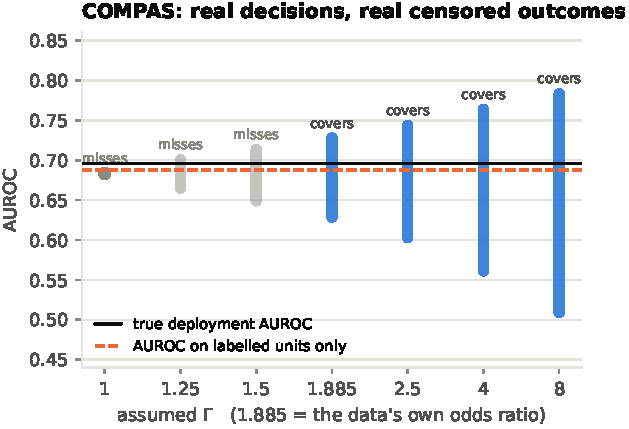
\includegraphics[width=0.5\linewidth]{figures/fig2_compas}
\caption{\textbf{Real pretrial release decisions with recorded censored
outcomes.} Intervals that contain the recorded deployment AUROC are drawn in
colour, those that miss it in grey. Assuming missing-at-random ($\Gamma=1$)
collapses the interval to a point that misses; coverage begins at the $\Gamma$
implied by the data's own detained-versus-released odds ratio,
$\nCompasOR$.}
\label{fig:compas}
\end{figure}

\Cref{fig:compas} checks the bounds against decisions no one simulated. The
recorded odds ratio between the detained and released groups' rearrest rates
is $\nCompasOR$. At $\Gamma=1$ --- the missing-at-random assumption that IPW
and AIPW require --- the interval collapses to a point and covers the recorded
AUROC in $\nCompasCovAtOne$ of splits. Coverage reaches $\nCompasCovAtOR$ at
$\Gamma=\nCompasOR$, where the interval has width $\nCompasWidthAtOR$: narrow
enough to be useful, wide enough to be honest. Corner evaluation covers in
$\nCompasCornerCovAtOR$ of splits at that $\Gamma$. Holding time at risk fixed
(\cref{app:compas-audit}) \emph{raises} the odds ratio to $\nCompasExpOR$ ---
incapacitation was masking selection, not creating it --- and coverage at that
anchor is $\nCompasExpCovAtOR$. \Cref{tab:main} repeats the method
comparison. The minimax-regret rule certifies a regret
$\nCompasRegretRatioErm\times$ tighter than ERM while its realised risk
($\nCompasMDclRegTwoRisk$) is lower than every baseline's except the
parametric selection model's, and lower than the \emph{oracle}'s
($\nCompasMOracleRisk$); Heckman's realised risk is also the least stable
across splits ($\nCompasMHeckmanRiskMin$--$\nCompasMHeckmanRiskMax$), as one
expects of identification that rests on a functional form. We read this as
the strongest available evidence that $\dcsm(\Gamma)$, with $\Gamma$ anchored
to leniency or odds-ratio structure, is the right object to report.



\subsection{The bounds are sharp, valid and cheap}
\label{sec:exp-sharp}

\begin{table}[t]
\centering\small
\caption{\textbf{Sharpness and validity of the AUROC interval} (SL-Bench,
$\nExpOneNCells$ cells of $(\Gamma_0,\Gamma)$ over $\Gamma_0\in\{1.5,2,3,5\}$,
$\Gamma\in\{1,\dots,8\}$, $\nExpOneSeeds$ seeds). Coverage is of the true
\emph{deployment} AUROC on held-out units. Corner evaluation is narrow because
it is wrong.}
\label{tab:sharpness}
\resizebox{\linewidth}{!}{\begin{tabular}{lccc}
\toprule
 & sharp (\cref{thm:sharp-auc}) & separate bounds & corner evaluation \\
\midrule
coverage when $\Gamma\ge\Gamma_0$ & $\mathbf{\nExpOneCovSharp}$ & $\nExpOneCovSeparate$ & $\nExpOneCovCorner$ \\
mean interval width               & $\nExpOneWidthSharp\pm\nExpOneWidthSharpCI$ & $\nExpOneWidthSeparate$ & $\nExpOneWidthCorner$ \\
coverage when $\Gamma<\Gamma_0$   & $\nExpOneCovTooSmall$ & --- & --- \\
\midrule
max $|$analytic $-$ brute force$|$ & \multicolumn{3}{c}{$\nExpOneGap$}\\
max $|\AUC(p^\star)-\text{bound}|$ (attainment) & \multicolumn{3}{c}{$\nExpOneAttain$}\\
runtime, $n=20{,}000$ / $100{,}000$ / $400{,}000$ & \multicolumn{3}{c}{$\nExpOneRuntimeTwentyK$s / $\nExpOneRuntimeHundredK$s / $\nExpOneRuntimeFourHundredK$s}\\
\bottomrule
\end{tabular}}
\end{table}

\Cref{tab:sharpness} tests \cref{thm:sharp-auc} three ways. \emph{Sharpness}:
an independent projected-gradient search over the identified box never escapes
the analytic interval and matches it to $\nExpOneGap$, while the extremal
$p^\star$ returned by the theorem lies in the box and attains the bound to
machine precision. \emph{Validity}: whenever $\Gamma\ge\Gamma_0$ the sharp
interval covers the deployment AUROC in $\nExpOneCovSharp$ of cells, degrading
to $\nExpOneCovTooSmall$ --- gracefully, not catastrophically --- when the
assumed $\Gamma$ is too small (\cref{app:misspec}). Corner evaluation covers in
$\nExpOneCovCorner$ of cells: it is $\nExpOneWidthRatioCorner\times$ narrower
than the sharp interval and, as \cref{prop:corner} predicts and
\cref{app:counterexample} exhibits, narrow for the wrong reason. Bounding
numerator and denominator separately is valid but
$\nExpOneWidthRatioSep\times$ wider, which is what sharpness buys.
\emph{Cost}: $400{,}000$ units in $\nExpOneRuntimeFourHundredK$ seconds.

\subsection{Decision-censored learning}
\label{sec:exp-learning}



\Cref{tab:main} (and \cref{fig:learning} in \cref{app:more-tables}) puts \cref{thm:dcl} and
\cref{prop:regret} against the field. \emph{The certificates.} DCL attains the
best worst-case risk on every testbed by construction; the margin is what
matters: $\nExpTwoLendingWcRatioErmOverDcl\times$ against ERM on Lending Club.
Certified regret separates the methods more sharply: the minimax-regret rule
\eqref{eq:regret-rule} cuts it by $\nExpTwoLendingRegretRatioErm\times$ against
ERM on Lending Club and $\nExpTwoSlBenchRegretRatioErm\times$ on SL-Bench.
The \emph{oracle}, fit on the uncensored labels, has poor certified regret: it
is tuned to one member of the identified set and is not robust to the others.
\emph{The realised metrics.} On Lending Club the two DCL rules also have the
lowest realised risk of any method, the oracle and the parametric selection
model included, and on COMPAS the minimax-regret rule is below every
baseline but Heckman and below the oracle --- not because they know more, but
because shrinking a calibrated estimate toward the decision boundary is a
better-conditioned estimator than fitting flexibly to labels. On SL-Bench, where the Heckman model's normality
assumption holds by construction, the parametric selection model attains the
best realised risk and DCL pays a small price for not assuming a functional
form. The minimax-\emph{risk} rule is uniformly more conservative; Manski
($\Gamma=\infty$) is valid and useless, with realised risk
$\nExpTwoLendingManskiRiskRatioErm\times$ ERM's on Lending Club.
\emph{The blind spot.} The observed AUROC differs from the deployment AUROC by
$\nExpTwoLendingErmObsMinusTrue$ on Lending Club and
$\nExpTwoSlBenchErmObsMinusTrue$ on SL-Bench; the sign differs between
testbeds, which is precisely why a sensitivity analysis is needed to know it.



\subsection{Falsifying $\Gamma$, break-even, generalisation and uncertainty}
\label{sec:exp-rest}

\begin{table}[t]
\centering\small
\caption{\textbf{Falsifying $\Gamma$ from leniency variation} (SL-Bench, 5
decision makers, 30 configurations). $\Gamma_0^{\mathrm{cond}}$ is the
\emph{within-decision-maker} sensitivity parameter, which is what
\cref{prop:falsify} bounds from below. ``Recovered'' is
$\log\Gamma_{\min}/\log\Gamma_0^{\mathrm{cond}}$ at the robust ($95$th
percentile) variant. The bound was valid in every one of the 30 cells, and never
refuted a true missing-at-random mechanism.}
\label{tab:falsify}
\begin{tabular}{cccccc}
\toprule
target $\Gamma_0$ & reliance on $S$ & $\Gamma_0^{\mathrm{cond}}$ &
$\Gamma_{\min}$ & $\Gamma_{\min}$ (q95) & recovered\\
\midrule
$1.0$ & homogeneous   & $1.000$  & $1.000$ & $1.000$ & --- \\
$1.0$ & heterogeneous & $1.000$  & $1.000$ & $1.000$ & --- \\
$1.5$ & homogeneous   & $1.582$  & $1.423$ & $1.341$ & $0.61$\\
$1.5$ & heterogeneous & $1.862$  & $1.573$ & $1.398$ & $0.51$\\
$2.0$ & homogeneous   & $2.273$  & $1.814$ & $1.594$ & $0.54$\\
$2.0$ & heterogeneous & $2.924$  & $2.181$ & $1.685$ & $0.45$\\
$3.0$ & homogeneous   & $3.831$  & $2.409$ & $1.914$ & $0.45$\\
$3.0$ & heterogeneous & $5.445$  & $3.164$ & $2.047$ & $0.39$\\
$5.0$ & homogeneous   & $7.623$  & $3.171$ & $2.270$ & $0.37$\\
$5.0$ & heterogeneous & $11.195$ & $4.420$ & $2.419$ & $0.34$\\
\bottomrule
\end{tabular}
\end{table}

\paragraph{The test never over-claims, and never cries wolf.}
\Cref{tab:falsify} reports $\Gamma_{\min}$ across 30 configurations varying the
true $\Gamma_0$, the spread of leniency, and whether decision makers rely on
their private information to the same degree. Two properties hold without
exception. First, \emph{validity}: $\Gamma_{\min}\le\Gamma_0^{\mathrm{cond}}$ in
every cell, as \cref{prop:falsify} requires. Second, \emph{no false alarms}: when
the mechanism really is missing-at-random the test returns exactly $1.000$ and
refutes nothing, so an analyst who runs it on genuinely unconfounded data is not
pushed into a needless sensitivity analysis.

\paragraph{How much it recovers.} \Cref{fig:falsify} plots every configuration
against the truth; on the log scale the test recovers $34$--$61\%$
of the truth, and --- as theory predicts --- less when decision makers differ in
\emph{how much} they use their private information rather than only in how
lenient they are: heterogeneity in reliance is exactly what makes different
decision makers' identified sets overlap for smaller $\Gamma$. So
$\Gamma_{\min}$ should be read as what it is: a floor the data will not let you
go below, not an estimate of $\Gamma_0$. At $\Gamma_0=3$ it already refutes
$\dcsm(\Gamma)$ for every $\Gamma<1.9$, which rules out missing-at-random ---
and with it IPW and AIPW --- decisively.

\begin{figure}[t]
\centering
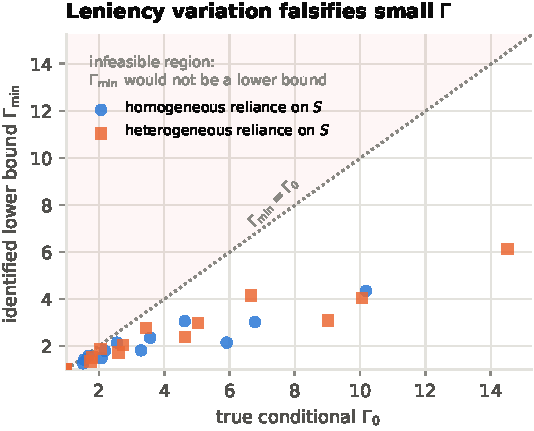
\includegraphics[width=0.58\linewidth]{figures/fig6_falsification}
\caption{\textbf{Every point lies below the diagonal:} the identified lower bound
never exceeds the true conditional $\Gamma_0$. Heterogeneous reliance on private
information across decision makers loosens the bound, as \cref{prop:falsify}'s
intersection argument predicts.}
\label{fig:falsify}
\end{figure}

\paragraph{Break-even analysis: what survives.}
The deliverable a practitioner wants is not a single interval but the $\Gamma$ at
which a conclusion flips. On Lending Club the incumbent model's AUROC lower bound
stays above $0.55$ up to $\Gamma=1.72$ and above chance up to $\Gamma=2.82$ ---
so the claim ``this model ranks better than chance'' survives past the true
$\Gamma_0=2.0$, while the stronger claim ``AUROC is at least $0.60$'' does not
survive even $\Gamma=1.05$. On MIMIC-sim, where the model is far more
discriminative, the above-chance claim survives to $\Gamma=14.9$. Separately, the
DCL model's certified worst-case risk beats the incumbent's at \emph{every}
$\Gamma$ we tested, up to $\Gamma=40$: the ordering of models under the
certificate is robust even where the absolute numbers are not.

\paragraph{When $\Gamma$ is set too small.} \Cref{tab:misspec} shows the failure
mode is graceful. Coverage is $100\%$ for every $\Gamma$ at least half the truth
and falls only to $69\%$ at $\Gamma\le\Gamma_0/2$, while the interval widens
monotonically and slowly --- from $0.04$ to $0.40$ over a $200$-fold range of
$\Gamma$. The price of a conservative $\Gamma$ is a wider interval, not a wrong
one; the price of an aggressive one is a graded loss of coverage, not a cliff.

\begin{table}[t]
\centering\small
\caption{\textbf{Coverage and width when the assumed $\Gamma$ is wrong}
(SL-Bench, 3 seeds, $\Gamma$ swept over a $200$-fold range).}
\label{tab:misspec}
\begin{tabular}{lcccccc}
\toprule
$\Gamma/\Gamma_0$ & $\le 0.5$ & $(0.5, 0.8]$ & $(0.8,1.0]$ & $(1.0,1.5]$ & $(1.5,3]$ & $>3$\\
\midrule
coverage & $0.69$ & $1.00$ & $1.00$ & $1.00$ & $1.00$ & $1.00$\\
mean width & $0.04$ & $0.14$ & $0.21$ & $0.26$ & $0.35$ & $0.40$\\
\bottomrule
\end{tabular}
\end{table}

\paragraph{Generalisation.} \Cref{thm:generalization} controls the uniform
deviation over the score class. On SL-Bench (\cref{app:scaling}) it decays with
exponent $\nExpFiveDevRate$ against the $-\tfrac12$ the bound predicts, every
cell in $[\nExpFiveRateMin,\nExpFiveRateMax]$. Regressing the fitted
$n^{-1/2}$ coefficient on $\log\Gamma$ gives $R^{2}=\nExpFiveRtwoLog$; on
$\Gamma$, $R^{2}=\nExpFiveRtwoLin$. Over a $\nExpFiveGammaRange$-fold range of
$\Gamma$ the coefficient grows by $\nExpFiveCoefGrowthPct\%$ --- consistent
with the $\log\Gamma$ of \cref{cor:loggamma} and not with a linear dependence,
which would predict more than an order of magnitude. The \emph{excess risk of
the empirical minimiser} decays much faster (exponent $\nExpFiveExcessRate$):
the familiar fast-rate phenomenon for a strongly convex objective, consistent
with an upper bound without being evidence for its rate, which is why we
measure the uniform deviation instead.

\paragraph{Uncertainty.} \Cref{fig:uq} and \cref{app:uq-table} separate three
things. \emph{Identification.} With oracle nuisances every claim of
\cref{cor:uq} holds: $p_1(x)$ lies inside the identified set for
$\nExpThreeOracleInBox$ of units at every $n$, and the naive aleatoric
estimate overstates the truth by $\nExpThreeAleaBias$ nats (about
$\nExpThreeAleaBiasRelPct\%$) while sitting inside the identified interval,
where no test on observed data can refute it. \emph{Asymptotic
overconfidence.} For a converged ensemble the reported epistemic term falls by
$\nExpThreeEpiDrop\times$ between $n=2{,}000$ and $n=70{,}000$ (fitted exponent
$\nExpThreeSlopeLog$), while the censoring term moves by
$\nExpThreeCensChangePct$ with no trend; at the largest sample the ratio is
$\nExpThreeRatioLast$: the reported uncertainty is two orders of magnitude
smaller than the identification uncertainty it omits. \emph{A
different, detectable pathology.} A fixed-budget deep ensemble's ``epistemic''
term does not contract (exponent $\nExpThreeSlopeMlp$) and exceeds the
censoring term throughout, but that is optimisation noise: its calibration
error is $\nExpThreeCalRatioMlpOverLog\times$ larger, and a calibration check
catches it, unlike the bias of \cref{cor:uq}.

\begin{figure}[t]
\centering
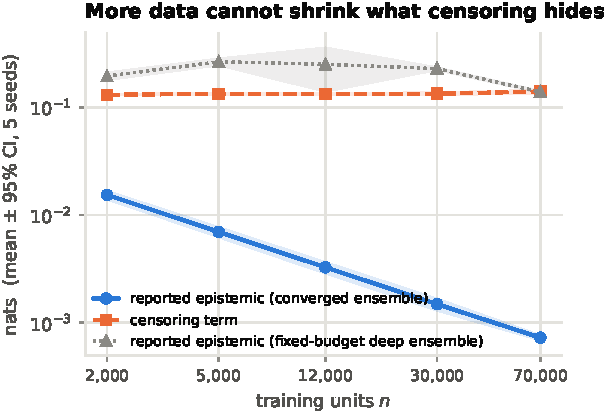
\includegraphics[width=0.58\linewidth]{figures/fig4_uq}
\caption{\textbf{More data cannot shrink what censoring hides}
(\cref{cor:uq}; $\nExpThreeSeeds$ seeds, 95\% bands). The reported epistemic
term of a converged ensemble collapses; the censoring term \eqref{eq:cens}
does not. A fixed-budget deep ensemble's term does not collapse either, for an
unrelated reason --- optimisation noise --- which a calibration check detects.}
\label{fig:uq}
\end{figure}


\section{Related work}
\label{sec:related}

\paragraph{Selective labels.} \citet{lakkaraju2017selective} named the problem
and proposed \emph{contraction}, which uses variation in decision-maker leniency
to construct a quasi-random subsample and estimate a model's failure rate at a
target acceptance rate; \citet{kleinberg2018human} applied the idea at scale to
bail. Contraction estimates a \emph{point} and requires the most lenient decision
maker to accept at least the target rate; it is silent about what happens outside
that decision maker's accepted set. \citet{dearteaga2018learning} exploit expert
consistency. Our contribution is orthogonal and complementary: we do not
estimate a point but characterise everything the data cannot rule out, and we
use leniency variation not to identify a risk but to \emph{falsify} a sensitivity
parameter (\cref{prop:falsify}).

\paragraph{Sensitivity analysis and partial identification.} $\dcsm(\Gamma)$ is
a decision-censoring form of Rosenbaum's bounds
\citep{rosenbaum1983assessing, rosenbaum2002observational} and is equivalent
(\cref{lem:msm}) to Tan's marginal sensitivity model
\citep{tan2006distributional}, for which sharp bounds and inference have been
developed for weighted averages and treatment effects
\citep{zhao2019sensitivity, yadlowsky2018bounds, dorn2023sharp}. Manski's
assumption-free bounds \citep{manski1990nonparametric, manski2003partial} are the
$\Gamma\to\infty$ endpoint. \citet{kallus2018confounding, kallus2021minimax}
develop confounding-robust \emph{policy} learning under the same model, which is
the closest antecedent to \cref{sec:learning}; their target is policy value under
a treatment assignment, ours is predictive risk under label censoring, and the
resulting objective --- midpoint risk plus a width-weighted margin penalty with a
closed-form Bayes act --- is different and, as we show, exactly convex without
relaxation. \citet{coston2021characterizing} and
\citet{rambachan2022counterfactual} study fairness and risk assessment under
selective labels and unmeasured confounding; \citet{jung2020algorithmic} give
related bounds for decision making. To our knowledge none of this literature
bounds a \emph{ranking} metric sharply, which is the gap \cref{thm:sharp-auc}
fills.

\paragraph{Missing data and sample selection.} Selective labels is
missing-not-at-random \citep{little2019statistical}. IPW and doubly robust
estimation \citep{robins1994estimation, chernozhukov2018double} require
missing-at-random --- exactly $\Gamma=1$ --- and we include both as baselines to
show what that costs when it fails. Parametric selection models
\citep{heckman1979sample, greene2012econometric} do permit selection on
unobservables, and we include the bivariate probit with partial observability as
the classical econometric comparator. The contrast is the point: it buys
identification with joint normality, an assumption that is untestable and not
indexed by any interpretable notion of strength, whereas $\Gamma$ is
interpretable, monotone, and --- with leniency variation --- falsifiable from
below.

\paragraph{Distributionally robust optimisation.} DRO minimises worst-case risk
over a ball around the empirical distribution
\citep{namkoong2016stochastic, duchi2021learning, sagawa2020distributionally}.
Formally \eqref{eq:dcl} is a DRO problem, but the ambiguity set is not a
modelling choice made for tractability: it is \emph{exactly what the observed
data fail to determine}, and its radius has a substantive interpretation. That
changes both the mathematics --- the inner supremum has a closed form and needs
no duality (\cref{rem:dro}) --- and the practice, since $\Gamma$ can be elicited
from domain experts and bounded below from data, whereas a divergence radius
cannot.

\paragraph{Ranking metrics.} The rank identity \eqref{eq:rank-identity} is a
population form of the Mann--Whitney representation of AUROC
\citep{mann1947test, hanley1982meaning}. Its use here --- to linearise AUROC in
the outcome regression at fixed prevalence, and thereby reduce a non-convex
bilinear-fractional optimisation over an identified set to a knapsack plus a
line search --- appears to be new.

\paragraph{Uncertainty quantification.} The aleatoric/epistemic decomposition
\citep{depeweg2018decomposition, hullermeier2021aleatoric} and deep ensembles
\citep{lakshminarayanan2017simple} assume the training labels are a sample from
the deployment law. \Cref{cor:uq} shows what breaks when a decision chose which
labels exist, and the credal-set decomposition we adopt follows
\citet{abellan2005difference}. The specific finding that the naive estimate is
\emph{never refutable} --- because $p_1(x)$ always lies inside the identified set
--- has, to our knowledge, not been noted.

\section{Discussion}
\label{sec:discussion}

\paragraph{What changes in practice.} Three things. First, a model evaluated on
selectively labelled data should report an \emph{interval}, and
\cref{thm:sharp-auc} makes the sharp one cheap enough ($400{,}000$ units in
$3.4$ seconds) that there is no excuse for the corner heuristic, which we show is
not a bound at all. Second, a model \emph{trained} on such data can be trained
against the identified set instead of against the labelled sub-population, at the
cost of one closed-form transformation of the nuisances --- and the
minimax-regret rule \eqref{eq:regret-rule} makes that nearly free in realised
performance. Third, reported uncertainty should carry a censoring component;
without it, more data makes a system more confident about a question it is not
answering.

\paragraph{Choosing $\Gamma$.} \Cref{thm:impossible} says this cannot be
avoided, so it should be done in the open. We suggest three inputs used
together: a lower bound from leniency variation where several decision makers
handle comparable cases (\cref{prop:falsify}); an anchor from any setting where
the censored outcomes happen to be recorded --- on COMPAS the realised odds ratio
between detained and released defendants is $1.9$, which is the order of
magnitude we would defend as a default in criminal justice; and a break-even
report saying at which $\Gamma$ each conclusion flips, which lets a reader who
disagrees with the analyst's number see immediately whether the disagreement
matters.

\paragraph{Limitations.} $\dcsm(\Gamma)$ is a bound on the \emph{worst} unit; it
permits every unit to be maximally tilted at once, which is conservative. The
budgeted variant (\cref{rem:budget}) and the directional variant
(\cref{rem:directional}) both relax this, and in our experiments the directional
version is where DCL improves realised deployment metrics rather than merely
certifying them --- but both require the analyst to supply more structure. The
bounds inherit whatever error is in $\hat e$ and $\hat p_1$; \cref{sec:experiments}
shows this is not negligible, and coverage guarantees are asymptotic in the
nuisance error even when exact in the identification. Our medical testbed is a
simulator, because MIMIC-IV is credentialed and could not be accessed from the
environment in which this work was produced; the loader against the real file
layout is implemented and documented, but the medical numbers reported here
should be read as a demonstration of the pipeline rather than as a clinical
finding. Finally, \cref{prop:falsify} needs random case assignment, which holds
in some courts and queues and not in others.

\paragraph{Outlook.} The rank identity \eqref{eq:rank-identity} is not specific
to selective labels: it linearises AUROC in the outcome regression under
\emph{any} constraint set, so sharp AUROC bounds should follow for covariate
shift, label noise and fairness-constrained model classes by substituting the
corresponding set for the box of \cref{lem:box}. On the learning side, the most
interesting open question is adaptive $\Gamma$: the identification width
$\delta(x)$ is a per-unit signal of how much the incumbent policy could be hiding
at $x$, and using it to direct \emph{data collection} --- deliberately labelling
where the identified set is widest --- turns the sensitivity model into an
acquisition function.


\bibliographystyle{plainnat}
\bibliography{refs}

\onecolumn
\appendix
\section{Proofs}
\label{app:proofs}

\subsection{Setup}
\label{app:setup}

\begin{proof}[Proof of \cref{lem:msm}]
Fix $x$. By a standard reduction (see e.g.\ \citealp{dorn2023sharp}), for the
purpose of bounding functionals of $\Prb(Y\mid X, T=0)$ the latent $S$ may be
replaced by $Y$ itself: the marginal sensitivity model with arbitrary latent $S$
and the model stated with $e(x,y)=\Prb(T=1\mid X=x, Y=y)$ generate the same set
of admissible observed-data-compatible laws. So assume
\begin{equation}
  \Lambda^{-1}
  \;\le\;
  \frac{\odds\big(e(x)\big)}{\odds\big(e(x,y)\big)}
  \;\le\;\Lambda,
  \qquad y\in\{0,1\}.
  \label{eq:msm-y}
\end{equation}
By Bayes' rule,
\[
  \odds\big(p_1(x)\big)
  = \frac{\Prb(Y=1\mid x)\,e(x,1)}{\Prb(Y=0\mid x)\,e(x,0)}
  = \odds\big(p(x)\big)\cdot\frac{e(x,1)}{e(x,0)},
  \qquad
  \odds\big(p_0(x)\big)
  = \odds\big(p(x)\big)\cdot\frac{1-e(x,1)}{1-e(x,0)} .
\]
Dividing,
\[
  \frac{\odds\big(p_0(x)\big)}{\odds\big(p_1(x)\big)}
  = \frac{(1-e(x,1))/e(x,1)}{(1-e(x,0))/e(x,0)}
  = \frac{\odds\big(e(x,0)\big)}{\odds\big(e(x,1)\big)} .
\]
By \eqref{eq:msm-y} each of $\odds(e(x,0))$, $\odds(e(x,1))$ lies in
$[\Lambda^{-1}\odds(e(x)),\,\Lambda\,\odds(e(x))]$, so their ratio lies in
$[\Lambda^{-2},\Lambda^{2}]$, which is \eqref{eq:dcsm} with $\Gamma=\Lambda^2$.
Attainment: take $e(x,1)$ at one end of its range and $e(x,0)$ at the other; both
choices are compatible with \eqref{eq:msm-y} and with the observed $e(x)$, so
every value in $[\Lambda^{-2},\Lambda^2]$ is realised.
\end{proof}

\begin{proof}[Proof of \cref{lem:box}]
Write $\eta_1(x)=\logit p_1(x)$. Given a tilt $a(\cdot)$, the induced regression
is \eqref{eq:tilt}, which is continuous and strictly increasing in $a(x)$ for
each $x$ with $e(x)<1$ (and constant, equal to $p_1(x)$, when $e(x)=1$). Hence
the image of $[\Gamma^{-1},\Gamma]$ under $a(x)\mapsto p^{a}(x)$ is exactly the
interval $[\plo(x),\pup(x)]$. Since $\dcsm(\Gamma)$ constrains $a$ only
\emph{pointwise} and $a$ is otherwise an arbitrary measurable function, the set of
achievable regressions is the product $\prod_x[\plo(x),\pup(x)]$, i.e.\ the
stated box. It is non-empty ($a\equiv1$ gives $p=p_1$), convex and compact
(a product of compact intervals, in the $L^\infty$ or weak topology as
appropriate). Nestedness and the two limits are immediate from monotonicity of
$\sigma$ and $\sigma(\pm\infty)=\{0,1\}$.
\end{proof}

\subsection{Ranking metrics}
\label{app:ranking}

\begin{proof}[Proof of \cref{thm:rank-identity}]
Let $(X,Y)$, $(X',Y')$ be independent with $X,X'\sim\mu$ and
$\Prb(Y=1\mid X)=p(X)$. From \eqref{eq:auc-def} the numerator is
\[
  N(p)=\iint \psi\big(f(x),f(x')\big)\,p(x)\,\big(1-p(x')\big)\,d\mu(x)\,d\mu(x').
\]
Define the operator $(\mathcal{K}h)(x)=\int\psi(f(x),f(x'))h(x')\,d\mu(x')$ on
$L^2(\mu)$, so $N(p)=\langle p, \mathcal{K}(\one-p)\rangle
= \langle p, \mathcal{K}\one\rangle - \langle p,\mathcal{K}p\rangle$ and
$\mathcal{K}\one = R$ by \eqref{eq:midrank}. Since
$\psi(u,v)+\psi(v,u)=1$ for all $u,v$ (including $u=v$, where both sides are
$\tfrac12+\tfrac12$), for any $g,h$
\[
  \langle g,\mathcal{K}h\rangle + \langle h,\mathcal{K}g\rangle
  = \iint\big[\psi(f(x),f(x'))+\psi(f(x'),f(x))\big]g(x)h(x')\,d\mu\,d\mu
  = \Big(\int g\,d\mu\Big)\Big(\int h\,d\mu\Big),
\]
i.e.\ $\mathcal{K}+\mathcal{K}^{*}=\one\otimes\one$. Taking $g=h=p$ gives
$2\langle p,\mathcal{K}p\rangle = \pi^{2}$, so
$\langle p,\mathcal{K}p\rangle = \pi^{2}/2$ for \emph{every} $p$. Hence
$N(p) = \langle p,R\rangle - \pi^2/2$, and dividing by
$\Prb(Y=1)\Prb(Y'=0)=\pi(1-\pi)$ gives \eqref{eq:rank-identity}.
\end{proof}

\begin{proof}[Proof of \cref{thm:sharp-auc}]
\emph{Reduction.} By \cref{lem:box} the identified set is the box $\I_\Gamma$.
Write $\Pi(p)=\E_\mu[p]$. For fixed $\pi\in(0,1)$ the denominator of
\eqref{eq:rank-identity} is a positive constant, so on the slice
$\{p\in\I_\Gamma : \Pi(p)=\pi\}$ the map $p\mapsto\AUC(p)$ is an increasing
affine function of $\E_\mu[pR]$. Therefore
\[
  \sup_{p\in\I_\Gamma}\AUC(p)
  = \sup_{\pi\in[\pi_-,\pi_+]}\ \sup_{\substack{p\in\I_\Gamma\\ \Pi(p)=\pi}}\AUC(p)
  = \sup_{\pi\in[\pi_-,\pi_+]}\frac{V^{+}(\pi)-\pi^2/2}{\pi(1-\pi)},
\]
and symmetrically for the infimum. The outer range is exactly $[\pi_-,\pi_+]$:
$\Pi$ is continuous on the connected set $\I_\Gamma$ with
$\Pi(\plo)=\pi_-$, $\Pi(\pup)=\pi_+$, so by the intermediate value theorem every
intermediate $\pi$ is attained, and no other value is.

\emph{(i) Structure of $V^{\pm}$.} Substituting $p=\plo + u$ with
$0\le u(x)\le \delta(x)$ turns the inner problem into a continuous
(fractional) knapsack: maximise $\E_\mu[uR]$ subject to $\E_\mu[u]=\pi-\pi_-$ and
$0\le u\le\delta$. The greedy solution --- saturate $u=\delta$ in decreasing
order of $R$ until the budget is spent, with at most one fractional unit ---
is optimal by the standard exchange argument. Its value as a function of the
budget is piecewise linear with slopes equal to the sorted $R$ values, which are
decreasing; hence $V^{+}$ is concave with at most $n$ breakpoints. For
$V^{-}$ the order is reversed and the slopes increase, giving convexity.

\emph{(ii) Stationary points.} On a linear piece write
$V^{\pm}(\pi)=\alpha+\beta\pi$ and $h(\pi)=N(\pi)/D(\pi)$ with
$N=\alpha+\beta\pi-\pi^2/2$ and $D=\pi-\pi^2$. Then
\[
  N'D-ND'
  = (\beta-\pi)(\pi-\pi^2) - \big(\alpha+\beta\pi-\tfrac{\pi^2}{2}\big)(1-2\pi)
  = \big(\beta-\tfrac12\big)\pi^{2} + 2\alpha\pi - \alpha,
\]
the $\pi^3$ terms cancelling identically. Setting this to zero gives the stated
quadratic. (The general form in \cref{prop:unified} follows by the same
expansion with $N=n_0+n_1\pi+n_2\pi^2$, $D=d_0+d_1\pi+d_2\pi^2$, yielding
$N'D-ND' = (n_1d_0-n_0d_1) + 2(n_2d_0-n_0d_2)\pi + (n_2d_1-n_1d_2)\pi^2$.)

\emph{(iii) Complexity.} Computing $R$ is a sort, $O(n\log n)$. Sorting by $R$
and forming the cumulative sums gives both profiles in $O(n\log n)$. Each of the
$\le n$ pieces contributes $O(1)$ candidate points (two endpoints, at most two
roots), each evaluated in $O(1)$, so the outer scan is $O(n)$.

\emph{Attainment.} The optimising $\pi^\star$ is attained (the objective is
continuous on the compact $[\pi_-,\pi_+]\cap(0,1)$ after the usual convention at
the degenerate ends), and the greedy construction returns an explicit
$p^\star\in\I_\Gamma$ with $\Pi(p^\star)=\pi^\star$ and
$\E_\mu[p^\star R]=V^{\pm}(\pi^\star)$. By \cref{lem:box} that $p^\star$
corresponds to an admissible tilt and hence to an admissible law.
\end{proof}

\begin{proof}[Proof of \cref{prop:corner}]
$\plo$, $\pup$ and $\tilde p$ all belong to $\I_\Gamma$, so their AUROC values
lie in the sharp interval and $\mathcal{C}$ is contained in it. For strictness,
consider the upper end. By the greedy characterisation, the maximiser at the
optimal prevalence sets $p=\pup$ on $\{R > r^\star\}$ and $p=\plo$ on
$\{R<r^\star\}$ for a pivot $r^\star$. If $R$ is non-constant on
$\{\delta>0\}$ this differs from $\plo$, $\pup$ and $\tilde p$ on a set of
positive measure; since $\E_\mu[pR]$ is strictly increasing in $p$ where $R>0$
and the objective is strictly increasing in $\E_\mu[pR]$ at fixed prevalence,
the maximum strictly exceeds all three corner values unless the optimal
prevalence coincides with one corner's prevalence \emph{and} the corner already
solves the knapsack, which requires $R$ constant on $\{\delta>0\}$. An explicit
three-point counterexample is given in \cref{app:counterexample}.
\end{proof}

\subsection{Learning}
\label{app:learning}

\begin{proof}[Proof of \cref{thm:dcl}]
\emph{(a)} By \cref{lem:box}, $\I_\Gamma$ is a product of intervals and
$R_P(f)=\E_\mu[p\,\ell_1+(1-p)\ell_0]$ is affine in $p(x)$ pointwise with slope
$\ell_1-\ell_0$. The supremum therefore decouples and is attained at
$\pup(x)$ where $\ell_1\ge\ell_0$ and at $\plo(x)$ otherwise:
\[
  \sup_{p\in\I_\Gamma}R_P(f)
  = \E_\mu\Big[\max\big\{\pup\ell_1+(1-\pup)\ell_0,\ \plo\ell_1+(1-\plo)\ell_0\big\}\Big].
\]
Apply $\max(A,B)=\tfrac{A+B}{2}+\tfrac{|A-B|}{2}$ with
$A-B=(\pup-\plo)(\ell_1-\ell_0)=\delta\,(\ell_1-\ell_0)$ to get
\eqref{eq:wc-decomp}. For the logistic loss
$\ell(z,1)-\ell(z,0)=\log(1+e^{-z})-\log(1+e^{z})=-z$, so $g_\ell(z)=|z|$.

\emph{(b)} For each fixed $p\in[0,1]$ the map
$z\mapsto p\,\ell(z,1)+(1-p)\ell(z,0)$ is a non-negative combination of convex
functions, hence convex. A pointwise supremum of convex functions is convex, so
$z\mapsto\max_{p\in[\plo,\pup]}\{\cdot\}$ is convex, and
$\Rbar_\Gamma(f)=\E_\mu[\cdot]$ is convex in $f$ as an element of any convex
class. For the second claim, subtracting the (convex) midpoint term from a
convex function leaves $\tfrac12\delta\,g_\ell$, which is convex iff $g_\ell$ is,
whenever $\delta$ may be taken constant and positive on a set of positive
measure. For the hinge loss $g_\ell(z)=2|z|$ on $|z|\le1$ and $1+|z|$ outside,
whose one-sided slopes at $z=1$ are $2$ then $1$: not convex.

\emph{(c)} $R_P(f)$ is convex in $f$ over the convex set $\F$ and affine --- hence
concave and continuous --- in $p$ over the convex compact $\I_\Gamma$. Sion's
minimax theorem \citep{sion1958general} gives $\inf\sup=\sup\inf$ and existence
of a saddle point; the adversary's best response is the vertex rule from part
(a). At a saddle point $\hat f$ minimises $R_{P^\star}(\cdot)$, i.e.\ it is the
Bayes predictor for $P^\star$.

\emph{(d)} Minimise $J(z)=\tilde p\,\zeta(-z)+(1-\tilde p)\zeta(z)
+\tfrac{\delta}{2}|z|$ pointwise, $\zeta(u)=\log(1+e^{u})$. For $z\neq0$,
$J'(z)=\sigma(z)-\tilde p+\tfrac{\delta}{2}\operatorname{sign}(z)$. On $z>0$,
$J'=0$ gives $\sigma(z)=\tilde p-\tfrac{\delta}{2}=\plo$, so
$z=\logit\plo$, admissible iff $\plo>\tfrac12$. On $z<0$, $J'=0$ gives
$\sigma(z)=\tilde p+\tfrac{\delta}{2}=\pup$, so $z=\logit\pup$, admissible iff
$\pup<\tfrac12$. Otherwise $0$ is a minimiser because the subdifferential at $0$
is $[\tfrac12-\pup,\ \tfrac12-\plo]$, which contains $0$ exactly when
$\plo\le\tfrac12\le\pup$. The three cases are exhaustive and mutually exclusive,
and $J$ is strictly convex, so the minimiser is unique.
\end{proof}

\begin{proof}[Proof of \cref{prop:regret}]
For the logistic loss and $q=\sigma(z)$,
$\E[\ell(z,Y)\mid p] - \inf_{z'}\E[\ell(z',Y)\mid p] = \KL(p\|q)$, so the
pointwise problem is $\min_{q}\max_{p\in[\plo,\pup]}\KL(p\|q)$. For fixed $q$,
$p\mapsto\KL(p\|q)$ is convex, so its maximum over an interval is attained at an
endpoint; the objective is thus
$\Psi(q)=\max\{\KL(\plo\|q),\KL(\pup\|q)\}$. Each branch is strictly convex in
$q$ with minimum $0$ at $q=\plo$ and $q=\pup$ respectively, the first increasing
in $q$ on $q>\plo$ and the second decreasing on $q<\pup$; hence on $(\plo,\pup)$
the two branches cross exactly once and $\Psi$ is minimised where they are equal
(for $\plo<\pup$). Setting $\KL(\plo\|q)=\KL(\pup\|q)$ and writing
$H(u)=-u\log u-(1-u)\log(1-u)$,
\[
  -H(\plo)-\plo\log q-(1-\plo)\log(1-q)
  \;=\;
  -H(\pup)-\pup\log q-(1-\pup)\log(1-q),
\]
so $H(\pup)-H(\plo) = (\plo-\pup)\log q + (\pup-\plo)\log(1-q)
= -(\pup-\plo)\logit q$, giving \eqref{eq:regret-rule}. As $\pup\downarrow\plo=p$
the right-hand side tends to $-H'(p)=\logit p$, recovering the precise case.
\end{proof}

\begin{proof}[Proof of \cref{cor:validity}]
Immediate: $P\in\I_\Gamma$ and $\Rbar_\Gamma(f)$ is the supremum of $R_{P'}(f)$
over $P'\in\I_\Gamma$.
\end{proof}

\subsection{Impossibility}
\label{app:impossibility}

\begin{proof}[Proof of \cref{thm:impossible}]
It suffices to exhibit two laws in $\mathcal{P}_{\Gamma,\eta}$ with identical
observed-data distributions and deployment risks differing by $\Delta$.

Let $P_X$ be arbitrary, let $e(x)=1-\eta$ so $\Prb(T=0)=\eta$, and fix any
$p_1(\cdot)$. Define two laws $P_{\pm}$ that agree on $(P_X, e, p_1)$ --- hence
on $P_{\mathrm{obs}}$, since the observed-data law is a function of exactly
$(P_X,e,p_1)$ and nothing else --- and differ in the censored branch:
\[
  \odds\big(p_0^{\pm}(x)\big) \;=\; \Gamma^{\pm1}\,\odds\big(p_1(x)\big).
\]
Both satisfy $\dcsm(\Gamma)$ with equality, so both lie in
$\mathcal{P}_{\Gamma,\eta}$. Their deployment risks satisfy
\[
  R_{P_+}(f)-R_{P_-}(f)
  = \E\Big[(1-e(X))\big(p_0^{+}(X)-p_0^{-}(X)\big)
    \big(\ell(f(X),1)-\ell(f(X),0)\big)\Big],
\]
whose absolute value is $\Delta$ as stated after noting that for
$p_1=\tfrac12$, $p_0^{+}-p_0^{-}=\tfrac{\Gamma}{\Gamma+1}-\tfrac{1}{\Gamma+1}
=\tfrac{\Gamma-1}{\Gamma+1}$ (for general $p_1$, replace this factor by the
corresponding difference, which is what the conditional expectation in
\eqref{eq:impossible} records).

Now let $\hat R_n$ be any estimator and set
$A=\{|\hat R_n - R_{P_-}(f)| < \Delta/2\}$. On $A^{c}$ the estimator errs by at
least $\Delta/2$ under $P_-$; on $A$, the triangle inequality gives
$|\hat R_n - R_{P_+}(f)| \ge \Delta - \Delta/2 = \Delta/2$, so it errs by at
least $\Delta/2$ under $P_+$. Because $P_{\mathrm{obs}}$ is the same under both
laws and $\hat R_n$ is a measurable function of the observed sample,
$\Prb_{P_-}(A)=\Prb_{P_+}(A)$. Hence
\[
  \max_{\pm}\Prb_{P_\pm}\!\big(|\hat R_n - R_{P_\pm}(f)|\ge\Delta/2\big)
  \;\ge\;
  \max\big\{1-\Prb_{P_-}(A),\ \Prb_{P_-}(A)\big\}
  \;\ge\;\tfrac12 .
\]
The argument uses no asymptotics, so the conclusion holds at every $n$.
\end{proof}

\begin{proof}[Proof of \cref{cor:gamma-unidentified}]
The observed-data law is determined by $(P_X, e, p_1)$, and $\dcsm(\Gamma)$
constrains only $p_0$, which does not enter it. So for every $\Gamma\ge1$ and
every observed-data law there exists a compatible $P$ (take $a\equiv1$). The
compatible sets coincide, and no test can have power.
\end{proof}

\begin{proof}[Proof of \cref{prop:falsify}]
Under \cref{ass:iv}, $Z\perp(Y,S)\mid X$ implies $\Prb(Y=1\mid X=x,Z=z)=p(x)$
for every $z$; applying \cref{lem:box} within each level $z$ gives
$p(x)\in[\plo_z^\Gamma(x),\pup_z^\Gamma(x)]$, hence membership in the
intersection. Each interval is continuous and nested increasing in $\Gamma$
(monotonicity of $\sigma$), so $\Gamma\mapsto\one\{\bigcap_z\neq\emptyset\}$ is
non-decreasing and the infimum defining $\Gamma_{\min}$ is attained and found by
bisection. Since the true $\Gamma_0$ makes the intersection non-empty (it
contains $p(x)$), $\Gamma_{\min}(x)\le\Gamma_0$. Finally, if
$\Gamma<\Gamma_{\min}(x)$ the intersection is empty, so no law satisfying
$\dcsm(\Gamma)$ conditionally on each $z$ can have generated the data, i.e.\
$\dcsm(\Gamma)$ is refuted.
\end{proof}

\subsection{Generalisation}
\label{app:generalization}

\begin{proof}[Proof of \cref{thm:generalization}]
Write $\bar\ell(z;x)=\max_{p\in[\plo(x),\pup(x)]}\{p\ell(z,1)+(1-p)\ell(z,0)\}$.

\emph{Lipschitzness.} For fixed $x$ the maximising $p$ is a vertex, and
$\partial_z[p\ell(z,1)+(1-p)\ell(z,0)]$ is a convex combination of
$\partial_z\ell(z,1)$ and $\partial_z\ell(z,0)$, each bounded by $L$; by Danskin's
theorem $\bar\ell(\cdot;x)$ is $L$-Lipschitz. For the logistic loss
$\partial_z\ell(z,1)=-\sigma(-z)\in[-1,0]$ and
$\partial_z\ell(z,0)=\sigma(z)\in[0,1]$, so $L=1$.

\emph{Uniform deviation.} $\bar\ell$ takes values in $[0,\ell_{\max}(B)]$ on
$\|f\|_\infty\le B$. By symmetrisation and Talagrand's contraction inequality
\citep{bartlett2002rademacher}, with probability $\ge1-\delta$,
\[
  \sup_{f\in\F}\big|\hat{\Rbar}^{\,\mathrm{oracle}}_\Gamma(f)-\Rbar_\Gamma(f)\big|
  \;\le\; 2L\,\Rad_n(\F)
  \;+\;\ell_{\max}(B)\sqrt{\tfrac{\log(2/\delta)}{2n}},
\]
where $\hat{\Rbar}^{\,\mathrm{oracle}}$ uses the true $(\plo,\pup)$. The standard
argument $\Rbar_\Gamma(\hat f) - \inf_\F\Rbar_\Gamma
\le 2\sup_\F|\hat{\Rbar}-\Rbar|$ doubles both terms.

\emph{Nuisance error.} $\bar\ell$ depends on $(\plo,\pup)$ through the affine
coefficient $\ell_1-\ell_0$, so
$|\bar\ell(z;\hat{\plo},\hat{\pup})-\bar\ell(z;\plo,\pup)|
\le \max(|\hat{\plo}-\plo|,|\hat{\pup}-\pup|)\cdot g_\ell(z)
\le \kappa(B)\max(|\hat{\plo}-\plo|,|\hat{\pup}-\pup|)$.
Both bounds are of the form $e\,p_1+(1-e)\sigma(\eta_1\mp\log\Gamma)$; the map
$(e,\eta_1)\mapsto\plo$ has partial derivatives bounded by
$|p_1-\sigma(\eta_1-\log\Gamma)|\le1$ in $e$ and by
$\sup|\sigma'|=\tfrac14$ in $\eta_1$, so
$|\hat{\plo}-\plo|\le|\hat e-e|+\tfrac14|\hat\eta_1-\eta_1|$, and likewise for
$\pup$. Taking expectations and doubling (again for the excess-risk argument)
gives the third term of \eqref{eq:gen-bound}. Note the bound is on the
\emph{logit} scale in $p_1$: this is where the $1$-Lipschitz behaviour of
$\Gamma$ as a translation is used.
\end{proof}

\begin{proof}[Proof of \cref{cor:loggamma}]
By \eqref{eq:bayes-act} the population optimum has
$|f^\star_\Gamma(x)|\le\max\{|\logit\plo(x)|,|\logit\pup(x)|\}$. Since
$\plo\ge e p_1 + (1-e)\sigma(\eta_1-\log\Gamma)$ and
$\pup\le e p_1 + (1-e)\sigma(\eta_1+\log\Gamma)$, monotonicity of $\logit$ and
$\logit\sigma(u)=u$ give $|\logit\pup|\le|\eta_1|+\log\Gamma\le B_0+\log\Gamma$
and symmetrically for $\plo$. Substituting $B=B_0+\log\Gamma$ and
$\ell_{\max}(B)\le\log2+B$, $\kappa(B)=B$ for the logistic loss into
\eqref{eq:gen-bound} gives \eqref{eq:loggamma}.
\end{proof}

\begin{proof}[Sketch of \cref{prop:lower-gen}]
Take $\X$ a single point, so $\F_\Gamma$ is the set of constants
$|z|\le B_0+\log\Gamma$, and let the identified set be
$[\plo,\pup]$ with $\pup<\tfrac12$ and $\logit\pup\asymp-(B_0+\log\Gamma)$. The
empirical objective is an average of $n$ i.i.d.\ terms whose range is
$\Theta(B_0+\log\Gamma)$ and whose minimiser must be located to accuracy
$\varepsilon$ in a loss that is locally quadratic with curvature bounded below;
a two-point argument on the Bernoulli parameter (Le Cam) then shows that
distinguishing the two candidate optima requires
$n = \Omega\big((\log\Gamma)^2/\varepsilon^2\big)$, i.e.\
$\varepsilon = \Omega(\log\Gamma\cdot n^{-1/2})$.
\end{proof}

\subsection{Uncertainty}
\label{app:uq}

\begin{proof}[Proof of \cref{cor:uq}]
\emph{(i)} $\plo = e p_1 + (1-e)\sigma(\eta_1-\log\Gamma)
\le e p_1 + (1-e)\sigma(\eta_1) = p_1$ since $\log\Gamma\ge0$ and $\sigma$ is
increasing; symmetrically $\pup\ge p_1$. So $p_1\in[\plo,\pup]$ always, with
strict interiority whenever $\Gamma>1$ and $e<1$.

\emph{(ii)} $H$ is concave on $[0,1]$ with maximum at $\tfrac12$, so on an
interval its maximum is at the point closest to $\tfrac12$ --- namely
$\mathrm{clip}_{[\plo,\pup]}(\tfrac12)$ --- and its minimum at whichever endpoint
is farther from $\tfrac12$, i.e.\ $\min\{H(\plo),H(\pup)\}$. Because
$\E_\mu[H(p)]$ is separable in $p(x)$ and the box is a product, the pointwise
extremes are simultaneously attainable, so the sharp interval for the mean is
the mean of the pointwise sharp interval.

\emph{(iii)} If $C_n(x)\to\{p_1(x)\}$ then both
$\max_{C_n}H$ and $\min_{C_n}H$ converge to $H(p_1(x))$, so the reported
epistemic term $\to0$. The censoring term \eqref{eq:cens} does not depend on $n$
and is positive whenever $\plo<\pup$, i.e.\ whenever $\Gamma>1$ and $e(x)<1$. For
the explicit bound, if $\tfrac12\notin[\plo,\pup]$ then $H$ is monotone there and
by the mean value theorem
$|H(\pup)-H(\plo)| = \delta\,|H'(\xi)| = \delta\,|\logit\xi|$
for some $\xi\in(\plo,\pup)$, which is at least
$\delta\cdot\min_{p\in[\plo,\pup]}|\logit p|$.
\end{proof}

\section{Generalisation under decision censoring}
\label{app:generalization-full}

We now bound the excess worst-case risk of the empirical minimiser. Let
$\F$ be a class of scores with $\|f\|_\infty\le B$, let
\[
  \hat{\Rbar}_\Gamma(f) = \frac1n\sum_{i=1}^{n}
  \max_{p\in[\hat{\plo}(x_i),\hat{\pup}(x_i)]}
  \big\{ p\,\ell(f(x_i),1) + (1-p)\,\ell(f(x_i),0) \big\},
  \qquad
  \hat f \in \argmin_{f\in\F}\hat{\Rbar}_\Gamma(f),
\]
and write $\Rad_n(\F)$ for the Rademacher complexity of $\F$.

\begin{theorem}[Excess worst-case risk]
\label{thm:generalization}
Assume $\ell$ is $L$-Lipschitz in its first argument with
$\sup_{|z|\le B,y}\ell(z,y)\le \ell_{\max}(B)$. Then with probability at least
$1-\delta$ over the sample,
\begin{equation}
  \Rbar_\Gamma(\hat f) - \inf_{f\in\F}\Rbar_\Gamma(f)
  \;\le\;
  4L\,\Rad_n(\F)
  \;+\;
  2\,\ell_{\max}(B)\sqrt{\frac{\log(2/\delta)}{2n}}
  \;+\;
  2\,\kappa(B)\Big(\|\hat e - e\|_{L^1(\mu)}
  + \tfrac14\|\hat\eta_1-\eta_1\|_{L^1(\mu)}\Big),
  \label{eq:gen-bound}
\end{equation}
where $\eta_1 = \logit p_1$ and $\kappa(B)=\sup_{|z|\le B} g_\ell(z)$.
For the logistic loss $L=1$, $\ell_{\max}(B)\le\log 2 + B$ and $\kappa(B)=B$.
\end{theorem}

The range $B$ is not free: to contain the population optimum
\eqref{eq:bayes-act} the class must reach $|\logit\pup|\le|\logit p_1|+\log\Gamma$,
so $B=B_0+\log\Gamma$ with $B_0\ge\sup_x|\logit p_1(x)|$ is necessary and
sufficient, and substituting gives

\begin{corollary}[$\log\Gamma$ scaling]
\label{cor:loggamma}
With $B=B_0+\log\Gamma$ and the logistic loss,
\begin{equation}
  \Rbar_\Gamma(\hat f) - \inf_{f\in\F_\Gamma}\Rbar_\Gamma(f)
  \;\le\;
  4\,\Rad_n(\F_\Gamma)
  \;+\;
  2\big(\log 2 + B_0 + \log\Gamma\big)\sqrt{\frac{\log(2/\delta)}{2n}}
  \;+\;
  2\big(B_0+\log\Gamma\big)\,\varepsilon_{\mathrm{nuis}},
  \label{eq:loggamma}
\end{equation}
i.e.\ the complexity term is \textbf{linear in $\log\Gamma$}, not in $\Gamma$.
\end{corollary}

On the probability scale the map from $p_1$ to the bounds has Lipschitz
constant $\Gamma$ and the bound would degrade multiplicatively; on the log-odds
scale $\Gamma$ is a translation, the map is $1$-Lipschitz, and only the score
range --- hence $\log\Gamma$ --- is affected.

\begin{proposition}[The $\log\Gamma$ dependence is necessary]
\label{prop:lower-gen}
There is a family of instances and a class $\F_\Gamma$ of constant scores with
$\|f\|_\infty\le B_0+\log\Gamma$ for which every estimator suffers excess
worst-case risk $\Omega\big(\log\Gamma\cdot n^{-1/2}\big)$. Hence
\eqref{eq:loggamma} is tight in its $\Gamma$-dependence up to constants.
\end{proposition}

Proofs are in \cref{app:generalization}; the empirical scaling is in
\cref{sec:experiments} and \cref{app:scaling}.

\section{Additional details}
\label{app:details}

\subsection{A three-point counterexample to corner evaluation}
\label{app:counterexample}

Let $\mu$ be uniform on three points with scores $f=(0,1,2)$, so the mid-ranks
\eqref{eq:midrank} are $R = (\tfrac16,\tfrac12,\tfrac56)$. Take the identified
box
\[
  \plo = (0.59,\;0.85,\;0.48),
  \qquad
  \pup = (0.98,\;0.98,\;0.97).
\]
Evaluating AUROC at the three natural corners gives
\[
  \AUC(\plo)=0.4470,\qquad \AUC(\tilde p)=0.4570,\qquad \AUC(\pup)=0.4512,
\]
so the corner recipe reports the interval $[0.4470,\,0.4570]$, of width $0.010$.
But the sharp interval of \cref{thm:sharp-auc} is $[0.1341,\,0.8252]$, of width
$0.691$. The witness for the upper end is the \emph{mixed} vertex
\[
  p^\star = (0.59,\;0.98,\;0.97) \in \I_\Gamma,
  \qquad \AUC(p^\star) = 0.8252,
\]
which takes $\plo$ at the lowest-ranked unit and $\pup$ at the two highest ---
precisely the greedy pattern of \cref{thm:sharp-auc}(i), and a point no corner
evaluation visits. The corner interval therefore misses an admissible law by
$0.368$ in AUROC. This is the mechanism behind the $10\%$ coverage reported in
\cref{sec:experiments}: corner evaluation is not a loose bound, it is not a
bound at all.

\subsection{Budgeted \texorpdfstring{$\dcsm$}{DCSM}}
\label{app:budget}

Under the additional constraint $\E|\log a(X)|\le B$ the inner supremum of
\eqref{eq:dcl} no longer decouples. Writing $t(x)=\log a(x)\in[-\log\Gamma,\log\Gamma]$
and $r(x,t)$ for the pointwise risk contribution at tilt $t$,
\[
  \sup_{\substack{|t|\le\log\Gamma\\ \E|t|\le B}} \E[r(X,t(X))]
  \;=\;
  \min_{\lambda\ge0}\ \Big\{\lambda B
  + \E\Big[\sup_{|t|\le\log\Gamma}\big\{r(X,t)-\lambda|t|\big\}\Big]\Big\},
\]
which decouples given $\lambda$; $\lambda$ is recovered by bisection on the
budget constraint. Strong duality holds because the primal is a supremum of a
linear objective over a convex compact set with the Slater point $a\equiv1$
(strictly feasible whenever $B>0$). The inner one-dimensional problem is solved
on a fixed grid of $t$, vectorised across units. The resulting worst-case risk
interpolates monotonically between the $\Gamma=1$ value and the pointwise
$\Gamma$ value as $B$ ranges over $[0,\log\Gamma]$.

\subsection{Worst-case-AUROC training}
\label{app:ranking-alg}

\begin{algorithm}[h]
\caption{\textsc{DCLRanker} --- worst-case AUROC by exact best response}
\label{alg:ranker}
\begin{algorithmic}[1]
\State \textbf{input} features $X$, identified box $[\plo,\pup]$, temperature
  $\tau$, steps $T$, oracle period $k$
\State $\theta \gets$ ridge fit to the midpoint $\tilde p$, normalised;
  $\bar p \gets \tilde p$; $\theta^{\text{best}}\gets\theta$
\State $v^{\text{best}} \gets \textsc{SharpAUCInterval}(X\theta,\plo,\pup).\text{lower}$
\For{$t=1,\dots,T$}
  \If{$t \equiv 0 \pmod k$}
    \State $p \gets \textsc{SharpAUCInterval}(X\theta,\plo,\pup).p_{\text{lower}}$
      \Comment{exact inner argmin, \cref{thm:sharp-auc}}
    \State $\bar p \gets \bar p + (p - \bar p)/(\text{\#responses})$
      \Comment{fictitious play: averaging prevents oscillation}
  \EndIf
  \State sample pairs $(i,j)$; $s \gets \sigma\big((x_i-x_j)^\top\theta/\tau\big)$
  \State $g \gets \overline{\bar p_i(1-\bar p_j)\,s(1-s)(x_i-x_j)}/\tau - \lambda\theta$
  \State $\theta \gets \Pi_{\|\theta\|=1}\big(\theta + \alpha_t\, g/\|g\|\big)$
  \State \textbf{if} the exact inner value at $\theta$ exceeds $v^{\text{best}}$
    \textbf{then} update $(\theta^{\text{best}}, v^{\text{best}})$
\EndFor
\State \textbf{return} $\theta^{\text{best}}$
\end{algorithmic}
\end{algorithm}

Because line 6 solves the inner minimisation \emph{exactly}, Danskin's theorem
makes the gradient in line 10 a valid supergradient of
$\min_{p\in\I_\Gamma}\AUC(\cdot,p)$ wherever the argmin is unique, and line 12
uses the same oracle to guarantee the returned model is no worse than its
initialisation.

Two implementation points, both learned the hard way. Best-responding to the
latest adversary rather than to the running average diverges: the exact inner
argmin sets $p=\plo$ where the current score ranks units high and $p=\pup$ where
it ranks them low, so the learner flips its ranking, the adversary flips back,
and the objective \emph{decreases} monotonically (in an early version, from
$0.467$ to $0.420$). Fictitious-play averaging fixes this. Second, the
normalisation $\|\theta\|=1$ is not cosmetic: AUROC is scale-invariant, so
without it the surrogate's effective temperature drifts with $\|\theta\|$ and the
gradient signal decays.

As reported in \cref{sec:learning}, the fixed algorithm converges but does not
beat its plug-in warm start on any instance we tried.

\subsection{Estimation of the nuisances}
\label{app:nuisance}

The bounds live on the probability scale, so \emph{calibration matters more than
discrimination}. We fit $\hat e$ and $\hat p_1$ with gradient-boosted trees
wrapped in isotonic calibration, using $K$-fold cross-fitting so that no unit's
identified set is built from a model that saw its own label --- the same reason
cross-fitting is standard in double machine learning
\citep{chernozhukov2018double}. $\hat p_1$ is fit on the selected units and
predicted for all units; for selected units we use out-of-fold predictions and
for censored units the average across folds. Propensities are clipped to
$[10^{-3},1-10^{-3}]$.

\Cref{thm:generalization}'s nuisance term is stated on the \emph{logit} scale for
$p_1$, which is what keeps the dependence on $\Gamma$ logarithmic; in the
implementation the bounds are likewise formed by translating
$\logit\hat p_1$ by $\pm\log\Gamma$ rather than by multiplying odds, for the same
numerical reason.

\subsection{Reproducibility}
\label{app:repro}

All public data are fetched by \texttt{scripts/download\_data.py} from the
Rdatasets archive and ProPublica's repository; the script prints SHA-256 digests.
MIMIC-IV is credentialed and is not redistributed: \texttt{dcl/data/mimic.py}
implements the full cohort-building pipeline against the real PhysioNet file
layout and documents the download, and \texttt{make\_mimic\_sim} provides the
simulator used for the numbers reported here. Every experiment script writes its
raw table and a JSON summary to \texttt{results/}. Random seeds are fixed and
reported; all figures regenerate from the saved tables.

\section{Additional results}
\label{app:more}

\subsection{Full method tables and confidence intervals}
\label{app:more-tables}

\Cref{tab:compas,tab:learning} give the full method lists behind
\cref{tab:main}, including observed AUROC and the imputation baseline;
\cref{tab:compas-ci,tab:learning-ci} give the half-widths of the 95\%
confidence intervals ($t$-based) for the two metrics the text compares, and
\cref{fig:learning} plots realised risk against certified regret.

\begin{table*}[h]
\centering\small
\caption{\textbf{Methods on COMPAS} --- real release decisions, recorded
censored outcomes, out of sample, $\nExpSixSeeds$ splits (mean; 95\% CIs in
\cref{app:more-tables}). Certificates are evaluated at $\Gamma=\nCompasOR$,
the recorded detained-versus-released odds ratio. Heckman is shown as the
range over splits.}
\label{tab:compas}
\begin{tabular}{lccccc}
\toprule
method & risk $\downarrow$ & AUROC $\uparrow$ & obs.\ AUROC & w.c.\ risk $\downarrow$ & regret $\downarrow$\\
\midrule
ERM-observed  & $\nCompasMErmRisk$ & $\nCompasMErmAuroc$ & $\nCompasMErmObsAuroc$ & $\nCompasMErmWc$ & $\nCompasMErmRegret$\\
IPW           & $\nCompasMIpwRisk$ & $\nCompasMIpwAuroc$ & $\nCompasMIpwObsAuroc$ & $\nCompasMIpwWc$ & $\nCompasMIpwRegret$\\
AIPW          & $\nCompasMAipwRisk$ & $\nCompasMAipwAuroc$ & $\nCompasMAipwObsAuroc$ & $\nCompasMAipwWc$ & $\nCompasMAipwRegret$\\
Imputation    & $\nCompasMImpRisk$ & $\nCompasMImpAuroc$ & $\nCompasMImpObsAuroc$ & $\nCompasMImpWc$ & $\nCompasMImpRegret$\\
Heckman probit & $\nCompasMHeckmanRiskMin$--$\nCompasMHeckmanRiskMax$ & $\nCompasMHeckmanAurocMin$--$\nCompasMHeckmanAurocMax$ & --- & $\nCompasMHeckmanWcMin$--$\nCompasMHeckmanWcMax$ & $\nCompasMHeckmanRegretMin$--$\nCompasMHeckmanRegretMax$\\
Manski ($\Gamma=\infty$) & $\nCompasMManskiRisk$ & $\nCompasMManskiAuroc$ & $\nCompasMManskiObsAuroc$ & $\nCompasMManskiWc$ & $\nCompasMManskiRegret$\\
DCL, minimax risk   & $\nCompasMDclTwoRisk$ & $\nCompasMDclTwoAuroc$ & $\nCompasMDclTwoObsAuroc$ & $\mathbf{\nCompasMDclTwoWc}$ & $\nCompasMDclTwoRegret$\\
DCL, minimax regret & $\mathbf{\nCompasMDclRegTwoRisk}$ & $\nCompasMDclRegTwoAuroc$ & $\nCompasMDclRegTwoObsAuroc$ & $\nCompasMDclRegTwoWc$ & $\mathbf{\nCompasMDclRegTwoRegret}$\\
\emph{oracle (uncensored)} & \emph{$\nCompasMOracleRisk$} & \emph{$\nCompasMOracleAuroc$} & --- & \emph{$\nCompasMOracleWc$} & \emph{$\nCompasMOracleRegret$}\\
\bottomrule
\end{tabular}
\end{table*}

\begin{table*}[h]
\centering\small
\caption{\textbf{Out-of-sample deployment metrics and certificates}, mean over
$\nExpTwoSeeds$ seeds (95\% CIs in \cref{app:more-tables}). \emph{Risk} and
\emph{AUROC} are on the complete outcomes of \emph{all} units; \emph{observed
AUROC} is what a practitioner would report; \emph{worst-case risk} and
\emph{regret} are certified at the instance's $\Gamma_0$
($\nExpTwoLendingGammaZero$ and $\nExpTwoSlBenchGammaZero$). Best in each
column in bold; the oracle is not attainable.}
\label{tab:learning}
\begin{tabular}{llccccc}
\toprule
& method & risk $\downarrow$ & AUROC $\uparrow$ & obs.\ AUROC & w.c.\ risk $\downarrow$ & regret $\downarrow$\\
\midrule
\multirow{7}{*}{\rotatebox{90}{Lending Club}}
& ERM-observed        & $\nExpTwoLendingErmRisk$ & $\nExpTwoLendingErmAuroc$ & $\nExpTwoLendingErmObsAuroc$ & $\nExpTwoLendingErmWc$ & $\nExpTwoLendingErmRegret$\\
& IPW                 & $\nExpTwoLendingIpwRisk$ & $\nExpTwoLendingIpwAuroc$ & $\nExpTwoLendingIpwObsAuroc$ & $\nExpTwoLendingIpwWc$ & $\nExpTwoLendingIpwRegret$\\
& AIPW                & $\nExpTwoLendingAipwRisk$ & $\nExpTwoLendingAipwAuroc$ & $\nExpTwoLendingAipwObsAuroc$ & $\nExpTwoLendingAipwWc$ & $\nExpTwoLendingAipwRegret$\\
& Heckman probit      & $\nExpTwoLendingHeckmanRisk$ & $\mathbf{\nExpTwoLendingHeckmanAuroc}$ & $\nExpTwoLendingHeckmanObsAuroc$ & $\nExpTwoLendingHeckmanWc$ & $\nExpTwoLendingHeckmanRegret$\\
& DCL, minimax risk   & $\nExpTwoLendingDclTwoRisk$ & $\nExpTwoLendingDclTwoAuroc$ & $\nExpTwoLendingDclTwoObsAuroc$ & $\mathbf{\nExpTwoLendingDclTwoWc}$ & $\nExpTwoLendingDclTwoRegret$\\
& DCL, minimax regret & $\mathbf{\nExpTwoLendingDclRegTwoRisk}$ & $\nExpTwoLendingDclRegTwoAuroc$ & $\nExpTwoLendingDclRegTwoObsAuroc$ & $\nExpTwoLendingDclRegTwoWc$ & $\mathbf{\nExpTwoLendingDclRegTwoRegret}$\\
& \emph{oracle}       & \emph{$\nExpTwoLendingOracleRisk$} & \emph{$\nExpTwoLendingOracleAuroc$} & --- & \emph{$\nExpTwoLendingOracleWc$} & \emph{$\nExpTwoLendingOracleRegret$}\\
\midrule
\multirow{7}{*}{\rotatebox{90}{SL-Bench}}
& ERM-observed        & $\nExpTwoSlBenchErmRisk$ & $\nExpTwoSlBenchErmAuroc$ & $\nExpTwoSlBenchErmObsAuroc$ & $\nExpTwoSlBenchErmWc$ & $\nExpTwoSlBenchErmRegret$\\
& IPW                 & $\nExpTwoSlBenchIpwRisk$ & $\nExpTwoSlBenchIpwAuroc$ & $\nExpTwoSlBenchIpwObsAuroc$ & $\nExpTwoSlBenchIpwWc$ & $\nExpTwoSlBenchIpwRegret$\\
& AIPW                & $\nExpTwoSlBenchAipwRisk$ & $\nExpTwoSlBenchAipwAuroc$ & $\nExpTwoSlBenchAipwObsAuroc$ & $\nExpTwoSlBenchAipwWc$ & $\nExpTwoSlBenchAipwRegret$\\
& Heckman probit      & $\mathbf{\nExpTwoSlBenchHeckmanRisk}$ & $\mathbf{\nExpTwoSlBenchHeckmanAuroc}$ & $\nExpTwoSlBenchHeckmanObsAuroc$ & $\nExpTwoSlBenchHeckmanWc$ & $\nExpTwoSlBenchHeckmanRegret$\\
& DCL, minimax risk   & $\nExpTwoSlBenchDclThreeRisk$ & $\nExpTwoSlBenchDclThreeAuroc$ & $\nExpTwoSlBenchDclThreeObsAuroc$ & $\mathbf{\nExpTwoSlBenchDclThreeWc}$ & $\nExpTwoSlBenchDclThreeRegret$\\
& DCL, minimax regret & $\nExpTwoSlBenchDclRegThreeRisk$ & $\nExpTwoSlBenchDclRegThreeAuroc$ & $\nExpTwoSlBenchDclRegThreeObsAuroc$ & $\nExpTwoSlBenchDclRegThreeWc$ & $\mathbf{\nExpTwoSlBenchDclRegThreeRegret}$\\
& \emph{oracle}       & \emph{$\nExpTwoSlBenchOracleRisk$} & \emph{$\nExpTwoSlBenchOracleAuroc$} & --- & \emph{$\nExpTwoSlBenchOracleWc$} & \emph{$\nExpTwoSlBenchOracleRegret$}\\
\bottomrule
\end{tabular}
\end{table*}

\begin{figure}[h]
\centering
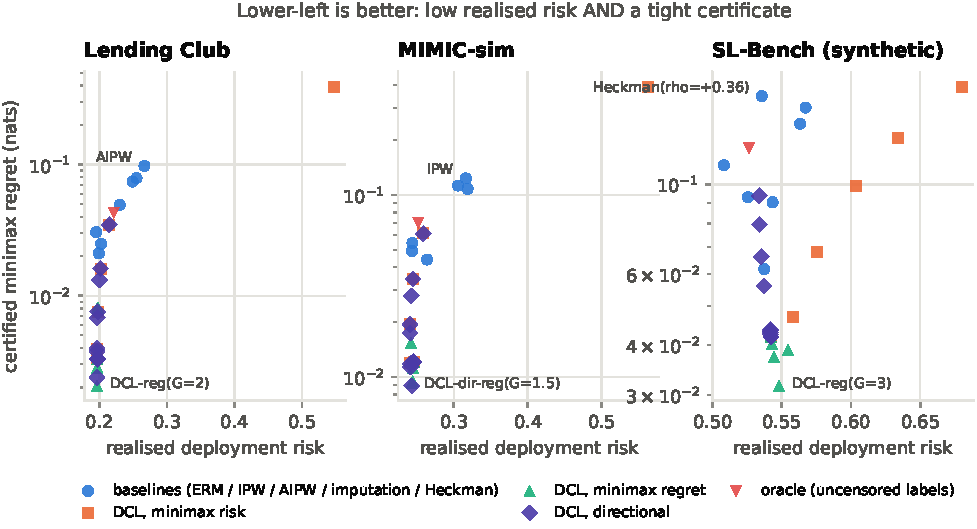
\includegraphics[width=\linewidth]{figures/fig3_learning}
\caption{\textbf{Realised deployment risk against certified minimax regret}
(log scale). Each point is a method; DCL variants are shown at several
$\Gamma$. The minimax-regret rule occupies the lower-left corner on every
testbed.}
\label{fig:learning}
\end{figure}

\begin{table*}[h]
\centering\small
\caption{COMPAS (recorded outcome): realised risk and certified regret with
95\% CIs over $\nExpSixSeeds$ splits.}
\label{tab:compas-ci}
\begin{tabular}{lcc}
\toprule
method & risk & regret\\
\midrule
ERM-observed & $\nCompasMErmRisk\pm\nCompasMErmRiskCI$ & $\nCompasMErmRegret\pm\nCompasMErmRegretCI$\\
IPW & $\nCompasMIpwRisk\pm\nCompasMIpwRiskCI$ & $\nCompasMIpwRegret\pm\nCompasMIpwRegretCI$\\
AIPW & $\nCompasMAipwRisk\pm\nCompasMAipwRiskCI$ & $\nCompasMAipwRegret\pm\nCompasMAipwRegretCI$\\
Imputation & $\nCompasMImpRisk\pm\nCompasMImpRiskCI$ & $\nCompasMImpRegret\pm\nCompasMImpRegretCI$\\
Heckman probit & $\nCompasMHeckmanRisk\pm\nCompasMHeckmanRiskCI$ & $\nCompasMHeckmanRegret\pm\nCompasMHeckmanRegretCI$\\
Manski & $\nCompasMManskiRisk\pm\nCompasMManskiRiskCI$ & $\nCompasMManskiRegret\pm\nCompasMManskiRegretCI$\\
DCL, minimax risk & $\nCompasMDclTwoRisk\pm\nCompasMDclTwoRiskCI$ & $\nCompasMDclTwoRegret\pm\nCompasMDclTwoRegretCI$\\
DCL, minimax regret & $\nCompasMDclRegTwoRisk\pm\nCompasMDclRegTwoRiskCI$ & $\nCompasMDclRegTwoRegret\pm\nCompasMDclRegTwoRegretCI$\\
oracle & $\nCompasMOracleRisk\pm\nCompasMOracleRiskCI$ & $\nCompasMOracleRegret\pm\nCompasMOracleRegretCI$\\
\bottomrule
\end{tabular}
\end{table*}

\begin{table*}[h]
\centering\small
\caption{Lending Club and SL-Bench: realised risk and certified regret with
95\% CIs over $\nExpTwoSeeds$ seeds.}
\label{tab:learning-ci}
\resizebox{\textwidth}{!}{\begin{tabular}{lcccc}
\toprule
 & \multicolumn{2}{c}{Lending Club} & \multicolumn{2}{c}{SL-Bench}\\
method & risk & regret & risk & regret\\
\midrule
ERM-observed & $\nExpTwoLendingErmRisk\pm\nExpTwoLendingErmRiskCI$ & $\nExpTwoLendingErmRegret\pm\nExpTwoLendingErmRegretCI$ & $\nExpTwoSlBenchErmRisk\pm\nExpTwoSlBenchErmRiskCI$ & $\nExpTwoSlBenchErmRegret\pm\nExpTwoSlBenchErmRegretCI$\\
IPW & $\nExpTwoLendingIpwRisk\pm\nExpTwoLendingIpwRiskCI$ & $\nExpTwoLendingIpwRegret\pm\nExpTwoLendingIpwRegretCI$ & $\nExpTwoSlBenchIpwRisk\pm\nExpTwoSlBenchIpwRiskCI$ & $\nExpTwoSlBenchIpwRegret\pm\nExpTwoSlBenchIpwRegretCI$\\
AIPW & $\nExpTwoLendingAipwRisk\pm\nExpTwoLendingAipwRiskCI$ & $\nExpTwoLendingAipwRegret\pm\nExpTwoLendingAipwRegretCI$ & $\nExpTwoSlBenchAipwRisk\pm\nExpTwoSlBenchAipwRiskCI$ & $\nExpTwoSlBenchAipwRegret\pm\nExpTwoSlBenchAipwRegretCI$\\
DCL, minimax risk & $\nExpTwoLendingDclTwoRisk\pm\nExpTwoLendingDclTwoRiskCI$ & $\nExpTwoLendingDclTwoRegret\pm\nExpTwoLendingDclTwoRegretCI$ & $\nExpTwoSlBenchDclThreeRisk\pm\nExpTwoSlBenchDclThreeRiskCI$ & $\nExpTwoSlBenchDclThreeRegret\pm\nExpTwoSlBenchDclThreeRegretCI$\\
DCL, minimax regret & $\nExpTwoLendingDclRegTwoRisk\pm\nExpTwoLendingDclRegTwoRiskCI$ & $\nExpTwoLendingDclRegTwoRegret\pm\nExpTwoLendingDclRegTwoRegretCI$ & $\nExpTwoSlBenchDclRegThreeRisk\pm\nExpTwoSlBenchDclRegThreeRiskCI$ & $\nExpTwoSlBenchDclRegThreeRegret\pm\nExpTwoSlBenchDclRegThreeRegretCI$\\
oracle & $\nExpTwoLendingOracleRisk\pm\nExpTwoLendingOracleRiskCI$ & $\nExpTwoLendingOracleRegret\pm\nExpTwoLendingOracleRegretCI$ & $\nExpTwoSlBenchOracleRisk\pm\nExpTwoSlBenchOracleRiskCI$ & $\nExpTwoSlBenchOracleRegret\pm\nExpTwoSlBenchOracleRegretCI$\\
\bottomrule
\end{tabular}}
\end{table*}

\begin{figure}[h]
\centering
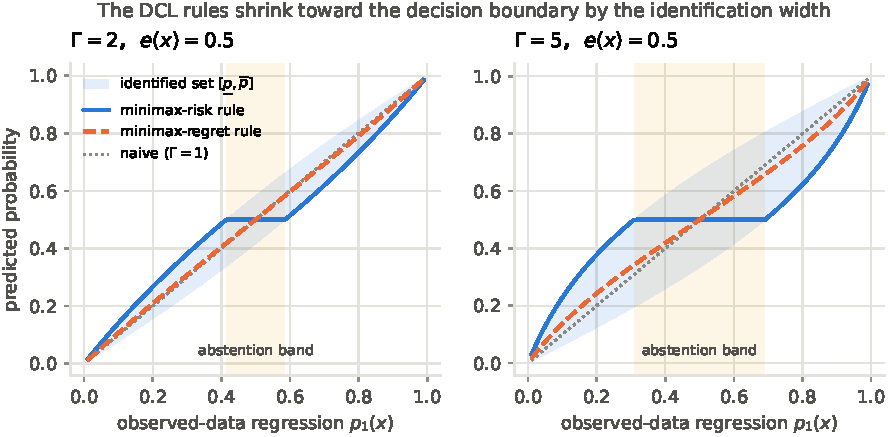
\includegraphics[width=0.7\linewidth]{figures/fig7_rules}
\caption{\textbf{The two closed-form DCL rules} (\cref{thm:dcl}(d) and
\cref{prop:regret}). Shaded: the identified set at $e(x)=0.5$. The
minimax-risk rule \eqref{eq:bayes-act} flattens to the decision boundary on
the abstention band; the minimax-regret rule \eqref{eq:regret-rule} stays
inside the identified set and remains a probability estimate throughout.}
\label{fig:rules}
\end{figure}

\subsection{COMPAS: lineage and time at risk}
\label{app:compas-audit}

\emph{Lineage.} ProPublica's \texttt{compas-scores-two-years.csv}
($n=\nCompasTarNRaw$) is filtered as in their analysis (screening within 30
days of arrest, ordinary-traffic offences and missing scores removed;
$n=\nCompasTarNPropublica$), then to units with jail dates and an index
custody spell of at most 180 days ($n=\nCompasTarNCohort$). $T=1$ is release
within two days of booking ($\nCompasTarSelectionPct$ of the cohort); the
median index custody is $\nCompasTarCustodyReleasedMedian$ days in the
released group and $\nCompasTarCustodyDetainedMedian$ days (90th percentile
$\nCompasTarCustodyDetainedQNinety$) in the detained group.

\emph{Time at risk.} Detention incapacitates: a defendant held for part of the
two-year window has less opportunity to be rearrested. ProPublica's survival
fields (\texttt{start}, \texttt{end}, \texttt{event}) give each unit's time
at risk in the community, so we also score \emph{rearrest within 730 days at
risk}, dropping units with neither an event nor 730 days of at-risk
follow-up ($\nCompasTarKeptPct$ kept; $\nCompasTarKeptDetainedPct$ of the
detained). The recorded detained/released rearrest rates are
$\nCompasTarPZeroRecorded$ vs.\ $\nCompasTarPOneRecorded$ (odds ratio
$\nCompasTarORRecorded$); with exposure held fixed they are
$\nCompasTarPZeroExposure$ vs.\ $\nCompasTarPOneExposure$ (odds ratio
$\nCompasTarORExposure$). The adjustment \emph{raises} the odds ratio:
incapacitation was masking selection on unobservables, not manufacturing it,
so the recorded anchor is, if anything, conservative. Under the
exposure-adjusted outcome the interval covers the recorded AUROC in
$\nCompasExpCovAtOR$ of splits at $\Gamma=\nCompasExpOR$ and in
$\nCompasExpCovAtOne$ at $\Gamma=1$; the minimax-regret rule's realised risk
is $\nCompasExpMDclRegTwoRisk\pm\nCompasExpMDclRegTwoRiskCI$ against ERM's
$\nCompasExpMErmRisk\pm\nCompasExpMErmRiskCI$ and the oracle's
$\nCompasExpMOracleRisk\pm\nCompasExpMOracleRiskCI$. Neither outcome is a
causal ground truth; both are recorded outcomes, and the paper's wording
follows that. The audit script is \texttt{audit/compas\_time\_at\_risk.py}.

\subsection{Lending Club: the hidden signal is kept out of $X$ by code}
\label{app:lending-guard}

The semi-synthetic construction is only meaningful if the underwriter's signal
$S$ (assigned interest rate and sub-grade) is absent from the learner's $X$.
\texttt{dcl.data.semisynthetic.assert\_hidden\_signal\_excluded} enforces this
at load time and raises otherwise: (i) no feature name matches the raw columns
$S$ is built from (\texttt{int\_rate}, \texttt{sub\_grade}, \texttt{grade});
(ii) no column of $X$ reproduces $S$ or a monotone transform of it (Pearson
and Spearman $|\rho|<0.95$ for every column); (iii) $S$ is not linearly
reconstructible from $X$ (in-sample $R^2<0.95$). The diagnostics are stored
with the dataset object and unit-tested (\texttt{tests/test\_data\_guards.py}).
The check guards against deterministic derivatives of $S$, not against
dependence between $S$ and $X$, which is expected and is what residualisation
removes before $\Gamma_0$ is calibrated.

\subsection{Falsification and misspecification tables}
\label{app:falsify}

\begin{table*}[h]
\centering\small
\caption{\textbf{Falsifying $\Gamma$ from leniency variation} (SL-Bench,
5 decision makers, $\nExpFourNCells$ configurations; each row averages the
leniency spreads). $\Gamma_0^{\mathrm{cond}}$ is the within-decision-maker
sensitivity parameter that \cref{prop:falsify} bounds from below;
``recovered'' is $\log\Gamma_{\min}/\log\Gamma_0^{\mathrm{cond}}$ at the
robust (95th percentile) variant.}
\label{tab:falsify}
\begin{tabular}{cccccc}
\toprule
target $\Gamma_0$ & reliance on $S$ & $\Gamma_0^{\mathrm{cond}}$ & $\Gamma_{\min}$ & $\Gamma_{\min}$ (q95) & recovered\\
\midrule
$1.0$ & homogeneous   & $\nExpFourOneHomGzCond$ & $\nExpFourOneHomGmin$ & $\nExpFourOneHomGminQ$ & ---\\
$1.0$ & heterogeneous & $\nExpFourOneHetGzCond$ & $\nExpFourOneHetGmin$ & $\nExpFourOneHetGminQ$ & ---\\
$1.5$ & homogeneous   & $\nExpFourOneFiveHomGzCond$ & $\nExpFourOneFiveHomGmin$ & $\nExpFourOneFiveHomGminQ$ & $\nExpFourOneFiveHomRec$\\
$1.5$ & heterogeneous & $\nExpFourOneFiveHetGzCond$ & $\nExpFourOneFiveHetGmin$ & $\nExpFourOneFiveHetGminQ$ & $\nExpFourOneFiveHetRec$\\
$2.0$ & homogeneous   & $\nExpFourTwoHomGzCond$ & $\nExpFourTwoHomGmin$ & $\nExpFourTwoHomGminQ$ & $\nExpFourTwoHomRec$\\
$2.0$ & heterogeneous & $\nExpFourTwoHetGzCond$ & $\nExpFourTwoHetGmin$ & $\nExpFourTwoHetGminQ$ & $\nExpFourTwoHetRec$\\
$3.0$ & homogeneous   & $\nExpFourThreeHomGzCond$ & $\nExpFourThreeHomGmin$ & $\nExpFourThreeHomGminQ$ & $\nExpFourThreeHomRec$\\
$3.0$ & heterogeneous & $\nExpFourThreeHetGzCond$ & $\nExpFourThreeHetGmin$ & $\nExpFourThreeHetGminQ$ & $\nExpFourThreeHetRec$\\
$5.0$ & homogeneous   & $\nExpFourFiveHomGzCond$ & $\nExpFourFiveHomGmin$ & $\nExpFourFiveHomGminQ$ & $\nExpFourFiveHomRec$\\
$5.0$ & heterogeneous & $\nExpFourFiveHetGzCond$ & $\nExpFourFiveHetGmin$ & $\nExpFourFiveHetGminQ$ & $\nExpFourFiveHetRec$\\
\bottomrule
\end{tabular}
\end{table*}

\begin{figure}[h]
\centering
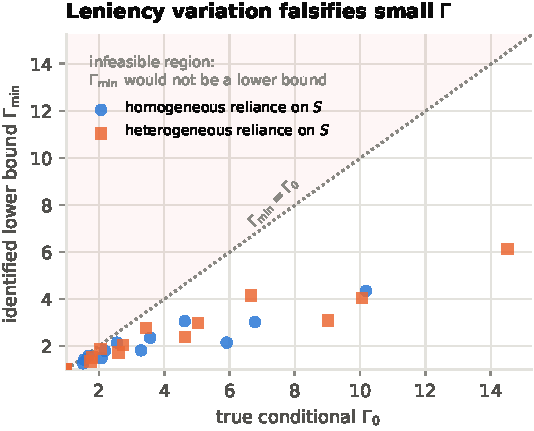
\includegraphics[width=0.5\linewidth]{figures/fig6_falsification}
\caption{\textbf{Every point lies below the diagonal:} the identified lower
bound never exceeds the true conditional $\Gamma_0$. Heterogeneous reliance on
private information loosens the bound, as \cref{prop:falsify}'s intersection
argument predicts.}
\label{fig:falsify}
\end{figure}

\label{app:misspec}
\emph{Misspecified $\Gamma$.} Over $\nExpFourMisSeeds$ seeds and a
$\nExpFourMisRange$-fold range of assumed $\Gamma$ on SL-Bench, coverage of the
deployment AUROC is $\nExpFourMisCovLow$ when $\Gamma\le\Gamma_0/2$ and
$\nExpFourMisCovHigh$ otherwise; the mean width rises monotonically from
$\nExpFourMisWidthMin$ at the smallest $\Gamma$ to $\nExpFourMisWidthMax$ at
the largest.

\subsection{Generalisation scaling}
\label{app:scaling}

\begin{table*}[h]
\centering\small
\caption{\textbf{Uniform deviation over the score class} --- the quantity
\cref{thm:generalization} bounds --- on SL-Bench, $\nExpFiveSeedsDev$ seeds per
cell. $B=B_0+\log\Gamma$ is the score range the class must reach to contain
the population optimum.}
\label{tab:scaling}
\begin{tabular}{lcccccc}
\toprule
$\Gamma$ & $1.5$ & $2$ & $3$ & $6$ & $12$ & $24$\\
\midrule
$B=B_0+\log\Gamma$ & $\nExpFiveOneFiveB$ & $\nExpFiveTwoB$ & $\nExpFiveThreeB$ & $\nExpFiveSixB$ & $\nExpFiveTwelveB$ & $\nExpFiveTwentyFourB$\\
rate exponent in $n$ & $\nExpFiveOneFiveRate$ & $\nExpFiveTwoRate$ & $\nExpFiveThreeRate$ & $\nExpFiveSixRate$ & $\nExpFiveTwelveRate$ & $\nExpFiveTwentyFourRate$\\
coefficient of $n^{-1/2}$ & $\nExpFiveOneFiveCoef$ & $\nExpFiveTwoCoef$ & $\nExpFiveThreeCoef$ & $\nExpFiveSixCoef$ & $\nExpFiveTwelveCoef$ & $\nExpFiveTwentyFourCoef$\\
\bottomrule
\end{tabular}
\end{table*}

\begin{figure}[h]
\centering
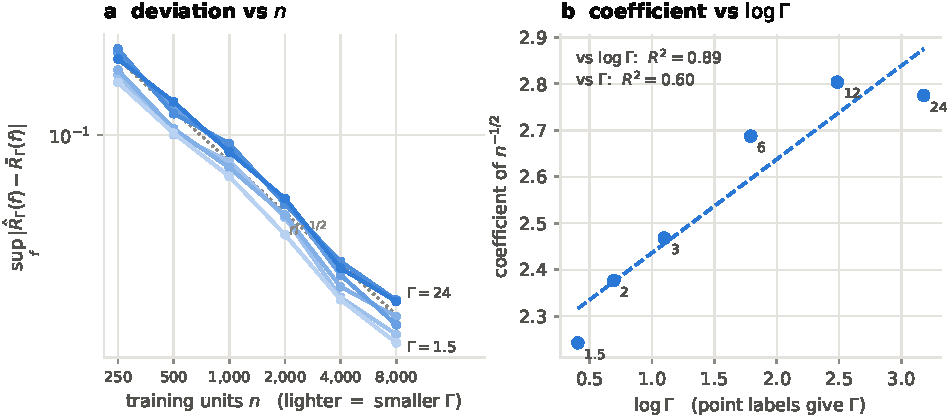
\includegraphics[width=0.8\linewidth]{figures/fig5_generalization}
\caption{\textbf{The generalisation bound in practice}
(\cref{thm:generalization}). (a) The uniform deviation decays at $n^{-1/2}$
for every $\Gamma$ (light to dark). (b) Its coefficient is well explained by
$\log\Gamma$ and poorly by $\Gamma$.}
\label{fig:scaling}
\end{figure}

\subsection{Uncertainty decomposition}
\label{app:uq-table}

\begin{table*}[h]
\centering\small
\caption{\textbf{The uncertainty decomposition under decision censoring}
(SL-Bench, in nats, $\nExpThreeSeeds$ seeds, mean $\pm$ 95\% CI). The
``converged'' ensemble is calibrated logistic regression run to convergence;
the ``fixed-budget'' one is a deep ensemble of MLPs trained for a fixed number
of epochs, the way they are usually built.}
\label{tab:uq}
\resizebox{\textwidth}{!}{\begin{tabular}{lccccc}
\toprule
$n$ & $2{,}000$ & $5{,}000$ & $12{,}000$ & $30{,}000$ & $70{,}000$\\
\midrule
epistemic, converged & $\nExpThreeEpiLogTwoK\pm\nExpThreeEpiLogTwoKCI$ & $\nExpThreeEpiLogFiveK\pm\nExpThreeEpiLogFiveKCI$ & $\nExpThreeEpiLogTwelveK\pm\nExpThreeEpiLogTwelveKCI$ & $\nExpThreeEpiLogThirtyK\pm\nExpThreeEpiLogThirtyKCI$ & $\nExpThreeEpiLogSeventyK\pm\nExpThreeEpiLogSeventyKCI$\\
epistemic, fixed-budget & $\nExpThreeEpiMlpTwoK\pm\nExpThreeEpiMlpTwoKCI$ & $\nExpThreeEpiMlpFiveK\pm\nExpThreeEpiMlpFiveKCI$ & $\nExpThreeEpiMlpTwelveK\pm\nExpThreeEpiMlpTwelveKCI$ & $\nExpThreeEpiMlpThirtyK\pm\nExpThreeEpiMlpThirtyKCI$ & $\nExpThreeEpiMlpSeventyK\pm\nExpThreeEpiMlpSeventyKCI$\\
censoring term \eqref{eq:cens} & $\nExpThreeCensTwoK\pm\nExpThreeCensTwoKCI$ & $\nExpThreeCensFiveK\pm\nExpThreeCensFiveKCI$ & $\nExpThreeCensTwelveK\pm\nExpThreeCensTwelveKCI$ & $\nExpThreeCensThirtyK\pm\nExpThreeCensThirtyKCI$ & $\nExpThreeCensSeventyK\pm\nExpThreeCensSeventyKCI$\\
ratio, converged & $\nExpThreeRatioTwoK$ & $\nExpThreeRatioFiveK$ & $\nExpThreeRatioTwelveK$ & $\nExpThreeRatioThirtyK$ & $\nExpThreeRatioSeventyK$\\
calibration error, converged & $\nExpThreeCalLogTwoK$ & $\nExpThreeCalLogFiveK$ & $\nExpThreeCalLogTwelveK$ & $\nExpThreeCalLogThirtyK$ & $\nExpThreeCalLogSeventyK$\\
calibration error, fixed-budget & $\nExpThreeCalMlpTwoK$ & $\nExpThreeCalMlpFiveK$ & $\nExpThreeCalMlpTwelveK$ & $\nExpThreeCalMlpThirtyK$ & $\nExpThreeCalMlpSeventyK$\\
\bottomrule
\end{tabular}}
\end{table*}

With estimated nuisances (cross-fitted gradient boosting, mean absolute error
$\nExpThreeNuisMaeMin$--$\nExpThreeNuisMaeMax$) the plug-in identified set
contains the true $p(x)$ for only $\nExpThreeEstBoxMin$--$\nExpThreeEstBoxMax$
of units, which is the phenomenon \cref{thm:nuisance} addresses.

\subsection{Nuisance-interval variants}
\label{app:nuisance-variants}

\begin{table}[h]
\centering\small
\caption{Per-unit coverage of $p(x)$ and mean box width for the binned
constructions of \cref{thm:nuisance}(c) with 10 or 20 bins, with and without
the within-bin oscillation margin ($\nExpEightSeeds$ seeds, mean $\pm$ 95\% CI).}
\label{tab:nuisance-variants}
\begin{tabular}{lcccc}
\toprule
 & \multicolumn{2}{c}{SL-Bench} & \multicolumn{2}{c}{Lending Club}\\
construction & coverage & width & coverage & width\\
\midrule
plug-in & $\nExpEightSlBenchCovPlugin\pm\nExpEightSlBenchCovPluginCI$ & $\nExpEightSlBenchWidthPlugin$ & $\nExpEightLendingCovPlugin\pm\nExpEightLendingCovPluginCI$ & $\nExpEightLendingWidthPlugin$\\
10 bins & $\nExpEightSlBenchCovBinsTen\pm\nExpEightSlBenchCovBinsTenCI$ & --- & $\nExpEightLendingCovBinsTen\pm\nExpEightLendingCovBinsTenCI$ & ---\\
20 bins & $\nExpEightSlBenchCovBinsTwenty\pm\nExpEightSlBenchCovBinsTwentyCI$ & $\nExpEightSlBenchWidthBinsTwenty$ & $\nExpEightLendingCovBinsTwenty\pm\nExpEightLendingCovBinsTwentyCI$ & $\nExpEightLendingWidthBinsTwenty$\\
10 bins + margin & $\nExpEightSlBenchCovBinsTenSmooth\pm\nExpEightSlBenchCovBinsTenSmoothCI$ & --- & $\nExpEightLendingCovBinsTenSmooth\pm\nExpEightLendingCovBinsTenSmoothCI$ & ---\\
20 bins + margin & $\nExpEightSlBenchCovBinsTwentySmooth\pm\nExpEightSlBenchCovBinsTwentySmoothCI$ & $\nExpEightSlBenchWidthBinsTwentySmooth$ & $\nExpEightLendingCovBinsTwentySmooth\pm\nExpEightLendingCovBinsTwentySmoothCI$ & $\nExpEightLendingWidthBinsTwentySmooth$\\
\bottomrule
\end{tabular}
\end{table}

\begin{figure}[h]
\centering
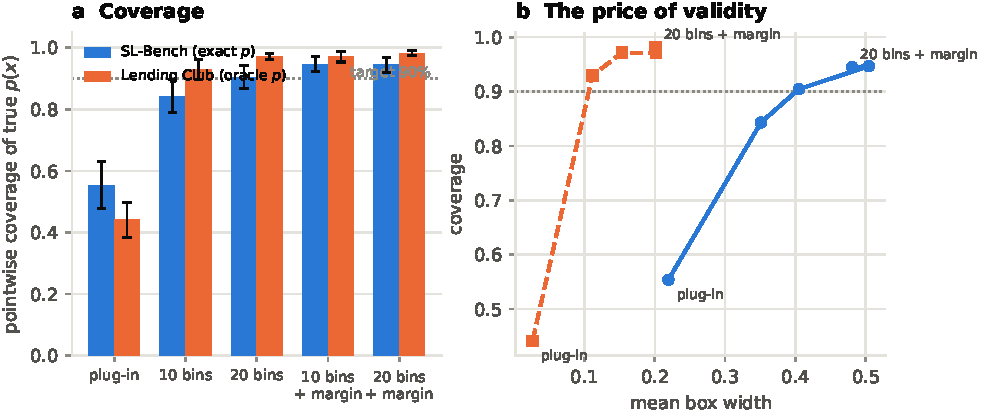
\includegraphics[width=0.8\linewidth]{figures/fig8_nuisance}
\caption{\textbf{Coverage under estimated nuisances} (\cref{thm:nuisance}):
per-unit coverage by construction and the width--coverage trade-off.}
\label{fig:nuisance}
\end{figure}

\subsection{Simulator validation}
\label{app:simulator}

A simulated emergency-department cohort (troponin ordering censors an acute
coronary syndrome label; \texttt{dcl/\allowbreak data/\allowbreak mimic.py}) is used only to check
that the pipeline behaves on a medical-shaped instance with a strong latent
signal; its numbers carry \texttt{data\_source:} \texttt{simulator} and appear nowhere
in the main text. At its $\Gamma_0=\nExpTwoMimicSimGammaZero$ the pattern of
\cref{tab:learning} repeats. Realised risk: ERM-observed
$\nExpTwoMimicSimErmRisk \pm \nExpTwoMimicSimErmRiskCI$, minimax-regret rule
$\nExpTwoMimicSimDclRegThreeRisk \pm \nExpTwoMimicSimDclRegThreeRiskCI$,
oracle $\nExpTwoMimicSimOracleRisk \pm \nExpTwoMimicSimOracleRiskCI$.
Certified regret: $\nExpTwoMimicSimErmRegret$ (ERM) against
$\nExpTwoMimicSimDclRegThreeRegret$ (minimax regret). Observed minus
deployment AUROC: $\nExpTwoMimicSimErmObsMinusTrue$. The above-chance claim
survives to $\Gamma=\nExpFourMimicSimBreakEvenFifty$.

\subsection{The real-data medical arm}
\label{app:medical}

The medical testbed of this paper is the MIMIC-IV-ECG $\times$ MIMIC-IV-ECHO
linkage: the unit is an ECG record, $T=1$ iff the same subject has an
echocardiogram within $\pm365$ days (the EchoNext protocol), restricted to
the echo coverage period, with $Y$ from structured echo measurements (eleven
structural heart disease phenotypes), discharge-summary extraction with a
manually validated sample as fallback, and ICD codes only as an auxiliary
outcome (circular with echo ordering, so appendix-only). The propensity is
estimated from an ECG encoder plus demographics and laboratory values,
cross-fitted and marginalised over the ordering department, and
$\Gamma_{\min}$ is obtained from department-level leniency. The pipeline
(\texttt{dcl/data/mimic\_ecg\_echo}, \texttt{experiments/exp7\_mimic\_ecg\_echo.py})
runs only against the credentialed files on the authors' server and exits
with a distinct error code when any is missing; it never substitutes a
simulator. Its numbers are \textbf{pending} that run and are not reported
here.

\section{Related-work matrix and extended discussion}
\label{app:related-matrix}

\begin{table*}[h]
\centering\scriptsize
\caption{\textbf{Positioning against the closest prior work.} ``Target'':
what is identified or bounded. ``Sharp'': bounds are attained by admissible
laws. ``Ranking'': a ranking metric (AUROC) is bounded. ``Learns'': a
predictor is trained against the identified set. ``$\Gamma$ testable'': the
sensitivity parameter can be bounded from data. ``Nuisance'': a coverage
statement under estimated nuisances is given.}
\label{tab:related}
\begin{tabular}{lllccccc}
\toprule
work & assumption & target & sharp & ranking & learns & $\Gamma$ testable & nuisance\\
\midrule
\citet{manski1990nonparametric} & none & mean outcome & yes & no & no & --- & no\\
\citet{rosenbaum2002observational} & $\Gamma$ on odds & test / effect & yes & no & no & no & no\\
\citet{lakkaraju2017selective} & leniency IV & failure rate at a target rate & point & no & no & --- & no\\
\citet{kallus2018confounding} & MSM($\Lambda$) & policy value & yes & no & policy & no & partial\\
\citet{dearteaga2018learning} & expert consistency & labels for censored units & no & no & yes & --- & no\\
\citet{coston2021characterizing} & MSM / IV & fairness metrics & yes & threshold & no & no & no\\
\citet{rambachan2022counterfactual} & IV / bounds & counterfactual risk & yes & no & no & partial & no\\
\citet{dorn2023sharp} & MSM($\Lambda$) & weighted means & yes & no & no & no & yes\\
\textbf{this paper} & $\dcsm(\Gamma)\equiv$ MSM($\Lambda^2$) & AUROC, risk, regret & yes & \textbf{yes} & \textbf{yes} & \textbf{lower bound} & \textbf{Thm.~5}\\
\bottomrule
\end{tabular}
\end{table*}

\subsection{Extended related work}
\label{app:related-full}

\Cref{tab:related} positions the paper. \emph{Selective labels.}
\citet{lakkaraju2017selective} named the problem and proposed contraction,
which uses leniency variation to estimate a model's failure rate at a target
acceptance rate; \citet{kleinberg2018human} applied it to bail;
\citet{dearteaga2018learning} exploit expert consistency. Contraction
identifies a point and needs the most lenient decision maker to accept at
least the target rate; we characterise everything the data cannot rule out and
use leniency to \emph{falsify} $\Gamma$ instead (\cref{prop:falsify}).
\emph{Sensitivity analysis.} $\dcsm(\Gamma)$ is a decision-censoring form of
Rosenbaum's bounds \citep{rosenbaum2002observational}, equivalent
(\cref{lem:msm}) to Tan's marginal sensitivity model \citep{tan2006distributional},
for which sharp bounds and inference exist for weighted averages and effects
\citep{zhao2019sensitivity, yadlowsky2018bounds, dorn2023sharp}; Manski's
bounds \citep{manski1990nonparametric} are the $\Gamma\to\infty$ endpoint.
\citet{kallus2018confounding} learn \emph{policies} robustly under the same
model, the closest antecedent to \cref{sec:learning}; their target is policy
value, ours predictive risk, and our inner supremum is closed-form without a
relaxation. \citet{coston2021characterizing} and
\citet{rambachan2022counterfactual} bound fairness metrics and counterfactual
risk under selective labels; none of this literature bounds a ranking metric
sharply, the gap \cref{thm:sharp-auc} fills, and none states per-unit coverage
under estimated nuisances, the gap \cref{thm:nuisance} addresses, using the
double-machine-learning product rate \citep{chernozhukov2018double}.
\emph{Missing data and DRO.} IPW and doubly robust estimation
\citep{robins1994estimation} require $\Gamma=1$; selection models
\citep{heckman1979sample} buy identification with joint normality. Formally
\eqref{eq:dcl} is a DRO problem \citep{duchi2021learning}, but the ambiguity
set is what the data fail to determine, not a modelling choice
(\cref{rem:dro}). \emph{Ranking and
uncertainty.} The rank identity is a population form of the Mann--Whitney
representation \citep{mann1947test, hanley1982meaning}, not previously used
to linearise AUROC in the outcome regression; the credal decomposition of
\cref{cor:uq} follows \citet{abellan2005difference} and contrasts with
ensembles \citep{lakshminarayanan2017simple, hullermeier2021aleatoric} that
assume the training labels sample the deployment law.


\end{document}
